\documentclass{fast-nuces-bs}
% The class loads natbib with "numbers, authoryear"; force numeric style for IEEEtran (replaces the Tectonic-only wrapper)
\setcitestyle{numbers,square}
%\documentclass{article}

\usepackage{blindtext}
\usepackage{mathptmx}% Times Roman font
\usepackage[T1]{fontenc}
\usepackage{lipsum} 
\usepackage{sectsty}
\usepackage{tikz-uml}
\usetikzlibrary{positioning,arrows.meta}
\usepackage{titlesec}
\usepackage{longtable}
\usepackage{booktabs}
\usepackage{pdflscape}
\usepackage{xurl}
\emergencystretch=2em

% Information about the Thesis 
% -----------------------------------------------------------------------------
% (All are compulsory, do not delete any line other than author Information)
% For e.g., usually there are 3 students in a group, so leave authorone, 
% authortwo, and authorthree, and delete authorfour.
%%%%%%%%%%%%%%%%%%%%%%%%%%%%%%%%%%%%%%%%%%%%%%%%%%%%%%%%%%%%%%%%%%%%%%%%%%%%%%%
\department{FAST School of Computing}
\faculty{Computer Science}
\degreeyear{2026}
\degreemonth{October}
\degreename{Computer Science}
\campuscity{Islamabad}
\authorone{Syed Sheharyar Ali}{23I-0097}
\authortwo{Maryam Fatima}{23I-3007}
\authorthree{Muhammad Ali Sajjad}{23I-0110}
\supervisor{Dr. Atif Aftab Ahmed Jilani}
\sessionduration{2023-2027}
\deanname{Dr. Jawwad Ahmed Shamsi}
\directorname{Dr. Waseem Shahzad}
\hodname{Dr. Muhammad Arshad Islam}
\fypcoordinatorname{FYP Coordinator}
% Administrative role names checked against official FAST-NUCES Islamabad pages on 10 October 2026.
% Dean: https://www.nu.edu.pk/University/Officers
% Director and HoD Computer Science: https://isb.nu.edu.pk/NEW/aboutCampus.php
\title{ASENT: Integrated Security Assurance for AI-Assisted Software Development}

% Connect the chapter fields to the FAST class metadata.
\makeatletter
\newcommand{\projecttitle}{\@title}
\newcommand{\studentone}{\@authoronename}
\newcommand{\studenttwo}{\@authortwoname}
\newcommand{\studentthree}{\@authorthreename}
\makeatother
%%%%%%%%%%%%%%%%%%%%%%%%%%%%%%%%%%%%%%%%%%%%%%%%%%%%%%%%%%%%%%%%%%%%%%%%%%%%%%%

%%%%%%%%%%%%%%%%%%%%%%%%%%%%%%%%%%%%%%%%%%%%%%%%%%%%%%%%%%%%%%%%%%%%%%%%%%%%%%
% Former document starts below this
\begin{document}

%\begin{acknowledgements}
%	Your acknowledgments here
%\end{acknowledgements}

%\begin{abstract}
%Briefly state the (1) research problem, (2) methodology, (3) key results, and (4) conclusion. Generally, abstracts are between 150 and 200 words–roughly 10-15 sentences.
%\end{abstract}

\chapter*{Students' Submission}
\addcontentsline{toc}{chapter}{Students' Submission}
We certify that this report is submitted as the FYP-1 mid-report for the project titled \textit{\projecttitle}.\par
\vspace{1cm}
\begin{center}
\begin{tabular}{p{0.45\textwidth}p{0.45\textwidth}}
Student 1: \studentone & Signature: \rule{0.25\textwidth}{0.4pt}\\[1cm]
Student 2: \studenttwo & Signature: \rule{0.25\textwidth}{0.4pt}\\[1cm]
Student 3: \studentthree & Signature: \rule{0.25\textwidth}{0.4pt}
\end{tabular}
\end{center}

\chapter*{Anti-Plagiarism Statement}
\addcontentsline{toc}{chapter}{Anti-Plagiarism Statement}
The students certify that this report is their own work and that all sources used in preparing the report have been appropriately acknowledged and referenced.

\chapter*{Authors' Declaration}
\addcontentsline{toc}{chapter}{Authors' Declaration}
We declare that the work documented in this report represents the work completed by the project team up to the FYP-1 mid-report stage. Contributions, tools, external components, and relevant sources are disclosed where applicable.

\chapter*{Abstract}
\addcontentsline{toc}{chapter}{Abstract}
AI-assisted software changes can alter dependencies, application code and infrastructure, and passing tests do not show that an existing security boundary still holds. ASENT (Agent Sentinel) is a local security-assurance gate that combines evidence from three modules into one decision of \texttt{ACCEPT}, \texttt{REVIEW} or \texttt{BLOCK}. CAVR checks dependency and capability evidence, SATRA-RV evaluates application-code changes against trusted tests and a sandboxed repair workflow, and SABLE checks whether a registered IAM/S3 obligation still holds on the successor of a protected Terraform resource after a refactor. SABLE's deterministic security decision path does not rely on an LLM. PR~\#5 integrated the three modules and shared gate into \texttt{master} at merge commit \texttt{ffe8aa91}; all 18 checks succeeded on its exact head \texttt{554b6d51}. The successful Core, SATRA, and SABLE workflow runs are recorded in Chapter~7. Those controlled checks do not establish live-cloud behavior or independent detection rates. FYP-2 will complete the agreed comparative evaluation, broaden validation where the research question supports it, and continue integrated testing.

\chapter*{Acknowledgments}
\addcontentsline{toc}{chapter}{Acknowledgments}
The project team acknowledges the guidance and support received from the project supervisor, faculty members, and other contributors.

\chapter*{Executive Summary}
\addcontentsline{toc}{chapter}{Executive Summary}

\section*{Project Motivation and Goal}
AI-assisted development can introduce changes across dependency manifests, application code, and infrastructure-as-code. A change may be syntactically valid while weakening a security control, changing the logical resource that a policy protects, or leaving insufficient evidence to make a trustworthy decision. ASENT (Agent Sentinel) is being developed as an assurance gateway between a proposed AI-assisted change and the point where that change is trusted, merged, or deployed. Its goal is to aggregate evidence from relevant security checks into a deterministic decision of \texttt{ACCEPT}, \texttt{REVIEW}, or \texttt{BLOCK}.

\section*{System Scope}
ASENT is organized around three security boundaries: CAVR addresses dependency security, SATRA-RV addresses application-code security, and SABLE addresses infrastructure security expressed through Terraform. The shared workflow combines module evidence and applies a final gate. This report's strongest verified implementation and contribution evidence concerns SABLE and the shared evidence/final-gate path. It does not treat the presence of other modules in the repository as proof of their authorship or complete readiness.

\section*{Implemented SABLE Approach}
SABLE analyzes supplied Terraform/\allowbreak{}HCL snapshots locally, builds a bounded resource/\allowbreak{}reference model, checks a registered baseline obligation, identifies a supported successor for the protected logical asset, and evaluates a bounded IAM/\allowbreak{}S3 authorization model against that successor. The outcome is explicit: \texttt{PRESERVED} when the registered obligation continues to hold, \texttt{REGRESSED} when supported evidence shows that it does not hold, or \texttt{UNKNOWN} when input semantics or resource correspondence are insufficient. In the shared workflow, current evidence is associated with the candidate snapshot and checked for freshness, input-\allowbreak{}hash consistency, and integrity before it contributes to the final decision.

\section*{Current Evidence}
PR~\#5 integrated the CAVR, SATRA-RV, and SABLE work into \texttt{master} at merge commit \texttt{ffe8aa91}; its exact tested head was \texttt{554b6d51}, and all 18 checks passed on that head. Representative Core, SATRA, and SABLE workflow runs are linked in Chapter~7. Separately, the focused SABLE/shared-assurance CI run on source commit \texttt{84f91a9} passed 48 tests, and the local focused selection on the correction-containing checkout passed 27 tests with 10 deselected. These results belong to their identified commits and are not a full-suite pass.

The 2026-10-12 post-merge shared-dashboard demonstration recorded SABLE \texttt{PRESERVED} in run \texttt{21adc601d6b7}, with overall \texttt{REVIEW} because SATRA was \texttt{INCONCLUSIVE}; the wrong-target run \texttt{0849603bfc16} recorded SABLE \texttt{REGRESSED} and overall \texttt{BLOCK}. Both traces showed valid integrity and matching candidate/input bindings. Their original screenshots are preserved under \path{report/evidence}; no AWS resources were applied or queried. This is a two-scenario demonstration, not full acceptance of every module.

An earlier rehearsal on \texttt{sable} commit \texttt{753a55b} recorded preserved, regressed, and unknown outcomes; the unknown screenshot was an intermediate capture, while its persisted final result was \texttt{REVIEW}. Those historical runs are described separately from the post-merge runs above.

\section*{Limitations and Remaining Work}
The SABLE analyzer supports a bounded subset of Terraform/HCL and IAM/S3 semantics. It does not apply Terraform, query deployed AWS state, or establish the full authorization behavior of AWS. The scenario fixtures are synthetic and authored in-house, so their results are not an independent estimate of real-world effectiveness. SATRA's \texttt{INCONCLUSIVE} status in the retained integrated run also remains visible evidence of an unresolved case, not a passing result.

For FYP-2, the proposed SABLE work is to complete the baseline comparison and broader validation, then extend supported cases only where the research question requires it. The team reports no outstanding proposal or panel actions and confirms that member contributions have been cross-checked. The report records those statements as team confirmations; no signed panel action register, meeting minutes, or approved FYP-2 schedule is represented as documentary evidence. The individual signature lines remain unsigned.

\chapter*{List of Abbreviations}
\addcontentsline{toc}{chapter}{List of Abbreviations}
\begin{tabular}{ll}
FYP & Final Year Project\\
FR & Functional Requirement\\
NFR & Non-Functional Requirement\\
\end{tabular}


\clearpage
\pagenumbering{arabic}
\chapter{Introduction and Project Vision}
\section{Project Overview}
ASENT (Agent Sentinel) is a local assurance workflow for reviewing security evidence associated with proposed software changes. The repository contains three module paths: CAVR for dependency analysis, SATRA-RV for application-code analysis, and SABLE for infrastructure-as-code analysis. This report section documents the verified SABLE contribution and does not infer authorship or readiness for the other modules from their presence in the repository.

\section{Problem Statement}
The SABLE problem is refactoring-induced security-boundary misbinding. A Terraform refactor can rename a resource, move it into a module, replace it, or introduce a competing resource. An IAM policy may remain syntactically valid and may grant the required actions, yet point to a different S3 bucket. A candidate-only policy check does not establish that the previously verified application-role obligation still protects the same logical data asset.

\section{Problem Context and Motivation}
The bounded case is the relationship between an application IAM role, a protected S3 customer-data bucket, and the required object actions. The authorization obligation is relational: principal, actions, and resource scope must all agree. Resource names and Terraform addresses can change during refactoring, so correspondence requires evidence beyond name similarity. This is a pre-deployment local analysis problem; the current prototype does not apply Terraform or query live AWS state.

\section{Project Vision}
ASENT's project vision is to combine attributable security evidence for proposed changes into a reviewable workflow decision. For SABLE, the mid-stage objective is narrower: check whether a registered S3/IAM obligation is preserved across supported Terraform changes, detect a known regression, and return uncertainty when available evidence cannot justify either conclusion.

\section{Project Objectives}
\begin{enumerate}
    \item Normalize the supported Terraform/HCL subset into resources, references, local-module outputs, and move records.
    \item Verify the registered obligation on the trusted baseline before making a continuity claim.
    \item Identify a supported successor using structural evidence and project the obligation onto it.
    \item Publish candidate-bound evidence for the shared gate and verify preserved, regressed, and uncertain outcomes with named tests.
\end{enumerate}

\section{Project Scope}
\begin{longtable}{p{0.22\textwidth}p{0.70\textwidth}}
\toprule
\textbf{In the current SABLE prototype} & \textbf{Explicit boundary}\\
\midrule
Local Terraform/HCL parsing for the supported resource subset, local modules and references; S3 buckets; selected inline IAM role-policy forms; baseline obligation checks; successor ranking; shared evidence freshness and final-gate integration. & No general Terraform interpreter, full AWS IAM evaluator, live AWS inspection, Terraform apply, arbitrary module expansion, production-scale performance claim, or independent real-world effectiveness result. Unsupported or unresolved semantics remain unknown.\\
\bottomrule
\end{longtable}

\section{Project Modules}
ASENT's repository organizes dependency, application-code, and Terraform/infrastructure analysis under CAVR, SATRA-RV, and SABLE respectively. The shared orchestrator routes relevant changes, stores module evidence, and evaluates a final decision. Detailed behavior and ownership claims in this report are limited to SABLE and the shared gate behavior demonstrated by its tests.

\section{Stakeholders and User Classes}
The intended users are project developers and reviewers who need an inspectable decision before trusting a proposed change. The supervisor and evaluation panel assess the prototype and its evidence. The team must confirm the contribution and administrative records required for the complete report.

\section{Success Criteria}
For this mid-stage SABLE scope, success is observable when: (i) a supported refactor preserving the registered obligation returns \texttt{PRESERVED}; (ii) a known wrong target or missing required action returns \texttt{REGRESSED}; (iii) an ambiguous successor, unresolved role binding, invalid baseline, or unsupported policy semantics does not return a safe verdict and instead returns \texttt{UNKNOWN}; and (iv) current SABLE evidence reaches the shared final gate with its candidate snapshot, input hash, and integrity checks intact. The requirement table and tests in Chapters 4 and 8 make these checks reproducible.

\section{Constraints and Assumptions}
The baseline and registered obligation are treated as trusted inputs supplied by the project configuration. SABLE's conclusions are limited to parsed evidence and its documented model. Synthetic fixtures support controlled regression tests but do not establish behavior on deployed AWS resources or independent production repositories. The analysis is local and requires no cloud credentials.

\section{Ethical, Legal and DEI Considerations}
The demonstrated analysis uses local fixture data and does not require personal data or cloud credentials. Reports must distinguish synthetic fixtures and static analysis from live infrastructure evidence. Tool-assisted development and team-wide disclosures require confirmation from the individuals concerned; this report records only the SABLE-related tool use verified for this report update.

\chapter{Research and Existing Solutions}

\section{Research Method / Approach}
This project examines a bounded infrastructure-assurance question: after a structural Terraform change, does a previously verified IAM authorization obligation remain attached to the intended logical Amazon S3 asset? The mid-stage work implements a deterministic analysis prototype and controlled scenario tests. It does not yet provide a completed comparative evaluation. Accordingly, the design and evidence below describe a research question and proposed evaluation, not a demonstrated advantage or a claim of novelty.

\section{Security Analysis of Infrastructure as Code}
Empirical work has studied whether security practices appear in IaC configurations and how practitioners use static-analysis findings. Verdet et al. analyze Terraform security-practice adoption across 812 open-source GitHub projects covering AWS, Azure, and Google Cloud. Their analysis uses configuration scanning and reports variation by practice category, including comparatively frequent access-policy practices and less frequent encryption-at-rest practices \cite{verdet2025terraform}. This establishes a broad empirical view of practice adoption in a public-repository sample. It does not study whether a specific verified authorization requirement remains associated with the same logical asset across a refactor, and its sample does not represent all deployed infrastructure.

Hu et al. characterize 491 static-analysis alerts from ten open-source Terraform repositories and one proprietary repository \cite{hu2023alerts}. They identify ten alert categories, five security-related, and examine practitioners' views of alert actionability and the relationship between resource dependencies and alert occurrence. This work shows that alert context and dependencies matter when interpreting scanner output. Its unit of analysis is the alert and practitioner response; it does not evaluate baseline-to-successor continuity of a particular IAM/S3 obligation. The repository count and one-company practitioner survey also bound how broadly its results can be generalized.

Together, these studies motivate automated IaC security checks while leaving a narrower continuity question open for this project to examine. They should not be read as evidence that existing scanners cannot address continuity: the studies' stated samples and research questions do not establish that comparison.

\section{Terraform Refactoring and Authorization Semantics}
Terraform's \texttt{moved} block records a prior and new resource or module address. Terraform checks state for the object at the prior address and updates its address before producing a plan, avoiding destruction solely due to the address change \cite{hashicorpMoved}. This provides explicit configuration-level evidence about address refactoring and state association. It does not, by itself, establish that an IAM policy's principal, actions, and resource scope still describe the intended protected asset after configuration changes.

That distinction matters for S3 because policy scope is expressed through resource identifiers: AWS documentation distinguishes bucket and object resources and describes the ARN forms used for each \cite{awsS3Policy}. A syntactically valid or locally compliant statement can still require interpretation against the intended bucket or object. Terraform address continuity, policy validity, and obligation-to-asset continuity are related but separate questions; the sources above do not claim to solve all three together.

\section{Research Gap and Proposed Evaluation}
The bounded gap investigated here is whether an analyzer can (1) verify a registered IAM/S3 obligation on a baseline snapshot, (2) identify a supported candidate successor after a Terraform structural change, and (3) evaluate whether the same obligation holds for that successor, returning uncertainty when correspondence or semantics are ambiguous. This is a project research question, not a proven gap across all prior work or a novelty claim. The internal research design defines the intended comparison and cautions that the claim should be narrowed if the method adds no useful evidence \cite{asentSableResearchDesign}.

The prototype's proposed evaluation compares the implemented B0--B4 configurations in \path{backend/sable/baselines.py} on controlled scenarios, including candidate-only checks, baseline verification, explicit move evidence, structural correspondence, and obligation projection. The scenarios can establish expected behavior for their stated fixtures; they do not substitute for an independently sampled benchmark. A defensible comparison must report its scenario construction, reference outcomes, errors and uncertainty, and limitations, and must avoid treating synthetic fixtures as live-cloud effectiveness. The current report records implementation and focused correctness evidence only: no completed comparative benchmark, independent effectiveness result, real-world error rate, or live deployment is claimed.

\section{Proposed Solution}
SABLE parses baseline and candidate snapshots, verifies the registered obligation on the baseline, ranks candidate successors using supported structural signals, evaluates the obligation on a unique supported successor, and emits \texttt{PRESERVED}, \texttt{REGRESSED}, or \texttt{UNKNOWN}. The shared workflow binds emitted evidence to the candidate snapshot and module input hash before the final gate uses it. Chapter 5 describes the implemented components; Chapter 8 presents their acceptance tests and evidence boundaries.

\section{Complex Computing Problem and Technical Challenges}
The problem combines declarative-language normalization, bounded resolution of references across local modules, successor selection among resources, and relational authorization evaluation. The analyzer must keep resource identity evidence separate from policy validity: a valid policy attached to an unrelated bucket must not be reported as preservation. Ambiguous or unsupported inputs therefore need an explicit uncertainty outcome. The implemented subset addresses HCL normalization, local-module references, structural correspondence, action/principal/resource checks, and evidence freshness and integrity; full Terraform evaluation, complete AWS policy semantics, and live cloud state remain outside scope.

\section{Research Findings and Design Decisions}
The literature establishes (a) observed adoption patterns for selected IaC security practices in public repositories, (b) alert categories and practitioner considerations for Terraform static analysis, (c) Terraform's address-refactoring behavior, and (d) AWS's distinction between policy resource scopes. It does not establish that SABLE improves on existing tools. Current local tests show that selected fixtures produce expected statuses; they do not demonstrate novelty, general effectiveness, or an independent error rate. The research contribution remains conditional on completing the planned comparison and reporting its results and limitations.

\chapter{Proposal Feedback and Iteration Plan}
\section{Proposal Feedback Summary}
The proposal panel feedback and completed Form 10/action register were not available in the repository or the report-source archive reviewed for this SABLE update. No feedback or action is inferred here. The team must obtain the authoritative panel record and complete this section and Appendix A before submission.
\section{Proposal Action Register}
\textbf{Pending team confirmation:} the blank rows below are template fields, not evidence that no actions were assigned. Populate them only from the actual panel feedback, with the action taken, owner, status, and evidence.
\begin{longtable}{p{0.06\textwidth}p{0.26\textwidth}p{0.23\textwidth}p{0.13\textwidth}p{0.16\textwidth}}
\toprule
No. & Feedback / Required Change & Action Taken & Status & Evidence\\
\midrule
1 & & & &\\
2 & & & &\\
3 & & & &\\
\bottomrule
\end{longtable}
\section{Iteration Strategy}
\begin{sloppypar}
For SABLE, work proceeded from a bounded obligation and fixtures to parser/correspondence behavior, authorization projection, and integration with shared evidence. Focused tests were used to verify the observable outcomes. The comparative FYP-2 experiments described in Chapter 10 are future work and are not counted as completed prototype milestones.
\end{sloppypar}
\section{Iteration 1 Plan}
\begin{sloppypar}
The SABLE mid-scope deliverables are: I1 candidate snapshot/input-hash/evidence-integrity binding; I2 supported Terraform/HCL normalization for modules, references, and tested inline IAM policies; I3 verification of the registered baseline obligation; I4 successor correspondence and explicit \texttt{PRESERVED}/\texttt{REGRESSED}/\texttt{UNKNOWN} results. Chapter 4 and Appendix B map these deliverables to test assertions. The initial published SABLE milestone was commit \texttt{9a4dc3d9}; the unresolved-role-binding correction followed in \texttt{58b0a3d}. Both are included in the verified combined snapshot at commit \texttt{665b224} on \texttt{integration/sable-satra-cavr}. This isolated integration branch has not been merged into \texttt{master}.
\end{sloppypar}
\section{Iteration 2 Plan}
Proposed SABLE continuation is to confirm the baseline comparison protocol, validate labels independently, execute the planned comparative evaluation, and broaden supported cases only where the research question requires it. No schedule, owner, or completed experiment is asserted here; the team and supervisor must confirm the plan.
\section{Work Breakdown and Responsibilities}
The repository evidence reviewed for this report supports the SABLE implementation and shared-gate contribution described in Chapter 9. A complete team task allocation, owner/date log, and contribution record for other modules were not verified in the source material reviewed. Confirm them against the team's records before submission.
\section{Progress Against Plan}
For SABLE I1--I4, the verified combined snapshot contains the snapshot/evidence path, supported normalization, baseline verification, successor selection, authorization projection, and explicit outcome tests. The earlier local selection reported 27 passed and 10 deselected; the initial published-commit CI reported 44 passed. The later shared-assurance CI on the combined commit reported 46 passed. These results are from distinct snapshots and runs; they establish selected checks, not completion of the later comparative research plan.
\section{Delays, Deviations and Recovery Plan}
The available evidence records no confirmed schedule baseline or approved delay/recovery log, so this report does not assign dates or declare a project-wide schedule deviation. The local test host's default pytest temporary directory was inaccessible; the selected tests passed using a fresh writable project-local \texttt{--basetemp}. Confirm any proposal-panel action or schedule impact from the team's official records.

\chapter{Software Requirements}
\begin{sloppypar}
This chapter states only the SABLE requirements that can be checked against the current implementation and tests. The obligation used for the acceptance cases is \texttt{S3-APPROLE-CUSTOMERDATA}: the registered application role must retain \texttt{s3:GetObject} and \texttt{s3:PutObject} on the protected customer-data bucket's object scope.
\end{sloppypar}

\section{User Interactions / Use Cases}
The reviewer supplies a baseline, a candidate Terraform snapshot, and the registered obligation; starts a SABLE run through the standalone or shared workflow; and inspects the verdict, reasons, and evidence. In the integrated workflow, the shared orchestrator stores SABLE evidence and reports the final gate decision.

\section{Use Case Diagram}
% Additive rubric artefact: use cases reflect the implemented dedicated SABLE page and shared Run Workflow.
\begin{figure}[htbp]
\centering
\begin{tikzpicture}[
  usecase/.style={draw, ellipse, align=center, text width=0.25\textwidth, minimum height=10mm, inner sep=2pt, font=\small},
  flow/.style={-{Stealth}, thick}
]
\node[draw, rounded corners, minimum width=0.78\textwidth, minimum height=84mm] (system) {};
\node[font=\small\bfseries, anchor=north] at ([yshift=-2mm]system.north) {Implemented ASENT analysis interfaces};
\coordinate (developer) at ([xshift=-0.55\textwidth,yshift=17mm]system.center);
\coordinate (reviewer) at ([xshift=0.55\textwidth,yshift=17mm]system.center);
\foreach \actor/\name in {developer/Developer,reviewer/Reviewer} {
  \draw (\actor) circle (2.3mm);
  \draw (\actor) -- ++(0,-8mm);
  \draw (\actor) ++(0,-3mm) -- ++(-4mm,-3mm);
  \draw (\actor) ++(0,-3mm) -- ++(4mm,-3mm);
  \draw (\actor) ++(0,-8mm) -- ++(-3mm,-5mm);
  \draw (\actor) ++(0,-8mm) -- ++(3mm,-5mm);
  \node[font=\scriptsize, below=18mm of \actor] {\name};
}
\node[usecase] (sable) at ([xshift=-0.26\textwidth,yshift=17mm]system.center) {Select obligation and baseline/candidate inputs};
\node[usecase, below=8mm of sable] (run) {Start standalone SABLE or shared analysis run};
\node[usecase] (inspect) at ([xshift=0.26\textwidth,yshift=17mm]system.center) {Inspect module status, reasons, and evidence};
\node[usecase, below=8mm of inspect] (decision) {Inspect shared final decision and evidence bindings};
\coordinate (dev-trunk-top) at ([xshift=-0.48\textwidth,yshift=17mm]system.center);
\coordinate (dev-trunk-bottom) at ([xshift=-0.48\textwidth,yshift=-17mm]system.center);
\coordinate (review-trunk-top) at ([xshift=0.48\textwidth,yshift=17mm]system.center);
\coordinate (review-trunk-bottom) at ([xshift=0.48\textwidth,yshift=-17mm]system.center);
\draw[flow] (developer) -- (sable.west);
\draw[flow] (developer) -- (dev-trunk-top) -- (dev-trunk-bottom) -- (run.west);
\draw[flow] (reviewer) -- (inspect.east);
\draw[flow] (reviewer) -- (review-trunk-top) -- (review-trunk-bottom) -- (decision.east);
\end{tikzpicture}
\caption{Implemented SABLE and shared-workflow use cases. The diagram shows user actions supported by the current interfaces; it does not imply live AWS access or deployment.}
\label{fig:asent-use-cases}
\end{figure}
The developer supplies supported analysis inputs and starts a run. A reviewer can inspect the module result, reasons, evidence, and (for the integrated route) the shared gate decision. The registered obligation is selected from the local SABLE interface; infrastructure is analyzed as supplied and is not applied to AWS.

\section{Detailed Use Cases}
\begin{enumerate}
    \item Assess a module refactor with one supported successor that still meets the baseline obligation.
    \item Assess a known wrong-target policy or a policy missing a required action.
    \item Assess ambiguous correspondence, unresolved role binding, invalid baseline, or unsupported policy semantics and preserve uncertainty.
    \item In the shared workflow, bind the SABLE result to current candidate evidence and map its status into the shared final decision.
\end{enumerate}

\section{Functional Requirements}
% Module FR files (each owned by its member, see OWNERS.md)
% OWNER: Maryam Fatima (Chapter 4 is shared; each member writes their module's FRs here)
\subsection{CAVR Functional Requirements}
% Numbered, testable FRs, e.g. FR-CAVR-01 ... with a one-line acceptance check each.

% OWNER: Syed Sheharyar Ali (Chapter 4 is shared; each member writes their module's FRs here)
\subsection{SATRA-RV Functional Requirements}
% Numbered, testable FRs, e.g. FR-SATRA-01 ... with a one-line acceptance check each.

\subsection{SABLE}
\setlength{\tabcolsep}{3pt}
\begin{longtable}{p{0.09\textwidth}p{0.34\textwidth}p{0.48\textwidth}}
\toprule
\textbf{ID} & \textbf{Requirement} & \textbf{Acceptance test and expected result}\\
\midrule
FR-S1 & Parse the supported Terraform/HCL snapshot, local modules, references, outputs, and explicit move records; expose unsupported constructs. & \path{test_sable_real_hcl}; \path{test_sable_unsupported_terraform_stays_unknown}. Supported cases parse; unsupported module expansion does not produce a safe result.\\
FR-S2 & Verify that a trusted, non-empty baseline satisfies the registered principal/action/resource obligation before claiming continuity. & \path{test_sable_real_hcl}; \path{test_sable_unverified_baseline_and_empty_baseline}; \path{test_shared_gate_reviews_missing_sable_baseline}. A supported baseline that satisfies the obligation permits continuity analysis; a failing, missing, or empty baseline yields SABLE \texttt{UNKNOWN} and cannot authorize final \texttt{ACCEPT}.\\
FR-S3 & Identify a unique successor from supported structural evidence and abstain when evidence conflicts or is ambiguous. & \path{test_sable_refactor_and_correspondence_cases}. Rename, move-into-module, and resolved move cases yield \texttt{PRESERVED}; competing candidates yield \texttt{UNKNOWN}.\\
FR-S4 & Evaluate principal, required actions, and resource scope on the selected successor. & \path{test_sable_real_hcl} and \path{test_sable_refactor_and_correspondence_cases}. A supported valid successor yields \texttt{PRESERVED}; wrong target or missing action yields \texttt{REGRESSED}.\\
FR-S5 & Do not treat unresolved role bindings, unsupported policy semantics, or untrusted evidence as proof of safety. & \path{test_sable_unsupported_iam_stays_unknown}; \path{test_sable_unresolved_role_binding_with_valid_policy_is_unknown}; \path{test_sable_standalone_evaluator_fails_closed_on_null_role_binding}; \path{test_sable_final_gate_requires_explicit_integrity_evidence}; \path{test_sable_final_gate_rejects_untrusted_evidence}. Unresolved cases yield SABLE \texttt{UNKNOWN}; missing, stale, mismatched, or invalid evidence yields final \texttt{REVIEW}, never \texttt{ACCEPT}.\\
\bottomrule
\end{longtable}
\setlength{\tabcolsep}{6pt}

\subsection{Shared Evidence and Gate}
\begin{longtable}{p{0.09\textwidth}p{0.35\textwidth}p{0.45\textwidth}}
\toprule
\textbf{ID} & \textbf{Requirement} & \textbf{Acceptance test and expected result}\\
\midrule
FR-S6 & Publish current SABLE evidence bound to the run's candidate snapshot and SABLE input hash, with valid integrity. & \path{test_shared_sable_evidence_drives_final_gate} asserts applicable SABLE evidence, snapshot equality, input-hash equality, and valid integrity.\\
FR-S7 & Map current valid SABLE statuses through the shared gate: preserved to accept, regression to block, uncertainty to review, subject to other applicable module evidence. & Parameter cases in \path{test_shared_sable_evidence_drives_final_gate} expect \texttt{PRESERVED}/\texttt{ACCEPT}, \texttt{REGRESSED}/\texttt{BLOCK}, and \texttt{UNKNOWN}/\texttt{REVIEW}; unresolved binding also expects \texttt{UNKNOWN}/\texttt{REVIEW}.\\
FR-S8 & Prevent stale, mismatched, or integrity-invalid evidence from establishing acceptance. & \path{test_sable_final_gate_rejects_untrusted_evidence}; stale snapshot, input-hash mismatch, invalid integrity, or stale evidence yields \texttt{REVIEW}.\\
\bottomrule
\end{longtable}
\setlength{\tabcolsep}{6pt}

\section{Non-Functional Requirements}
\subsection{Reliability}
For the supported cases, analysis must produce a reproducible explicit status, and unsupported semantics must not silently become a safe verdict. This is fixture-tested; it is not a quantified production reliability claim.
\subsection{Usability}
The standalone and integrated interfaces expose a verdict and supporting reasons/evidence for review. A live demonstration remains necessary for the presentation rubric.
\subsection{Performance}
No latency or scale target has been established in the evidence reported here. Performance measurement remains future evaluation work.
\subsection{Security}
The SABLE decision path is local and does not apply Terraform or call AWS. Shared evidence is bound to the candidate snapshot and module input hash and checked for integrity. The evaluator is bounded, not a full AWS authorization engine.

\section{Acceptance Criteria}
\begin{sloppypar}
\begin{itemize}
    \item \textbf{AC-S1 (PRESERVED):} a valid trusted baseline and unique supported successor retain the required principal, actions, and S3 object scope; tests assert \texttt{PRESERVED}.
    \item \textbf{AC-S2 (REGRESSED):} supported evidence establishes a wrong target or a missing required action; tests assert \texttt{REGRESSED}, not a local-policy-only safe result.
    \item \textbf{AC-S3 (UNKNOWN):} ambiguous correspondence, unresolved binding, unsupported policy semantics, or unverified baseline prevents a justified safe verdict; tests assert \texttt{UNKNOWN}.
    \item \textbf{AC-S4 (shared gate):} current integrity-valid evidence maps to \texttt{ACCEPT}/\texttt{BLOCK}/\texttt{REVIEW} according to SABLE status, while stale or untrusted evidence cannot establish acceptance.
\end{itemize}
\end{sloppypar}

\section{Requirements Traceability}
\begin{sloppypar}
FR-S1--S5 map to SABLE I2--I4 and the analyzer/parser/correspondence/authorization components. FR-S6--S8 map to I1 and the shared orchestrator/final gate. The named test files and direct expected values are listed in Appendix C. The four local shared-integration parameter cases are one parameterized test function; test counts reported in Chapter 8 must not be read as the count of distinct requirements.
\end{sloppypar}

\chapter{System Design}
\section{System Architecture}
The React frontend calls FastAPI routes. The shared service orchestrator freezes the candidate, routes applicable analyzers, stores their evidence and events, and asks the shared final gate to validate current bindings and compute the workflow result. Module-specific interfaces remain available in addition to the shared Run Workflow. Figure~\ref{fig:asent-overall-architecture} is page 02 of the editable diagrams.net source \texttt{ASENT\_All\_Diagrams.drawio}; its labels and flow correspond to the current local application.

\begin{landscape}
\begin{figure}[p]
\centering
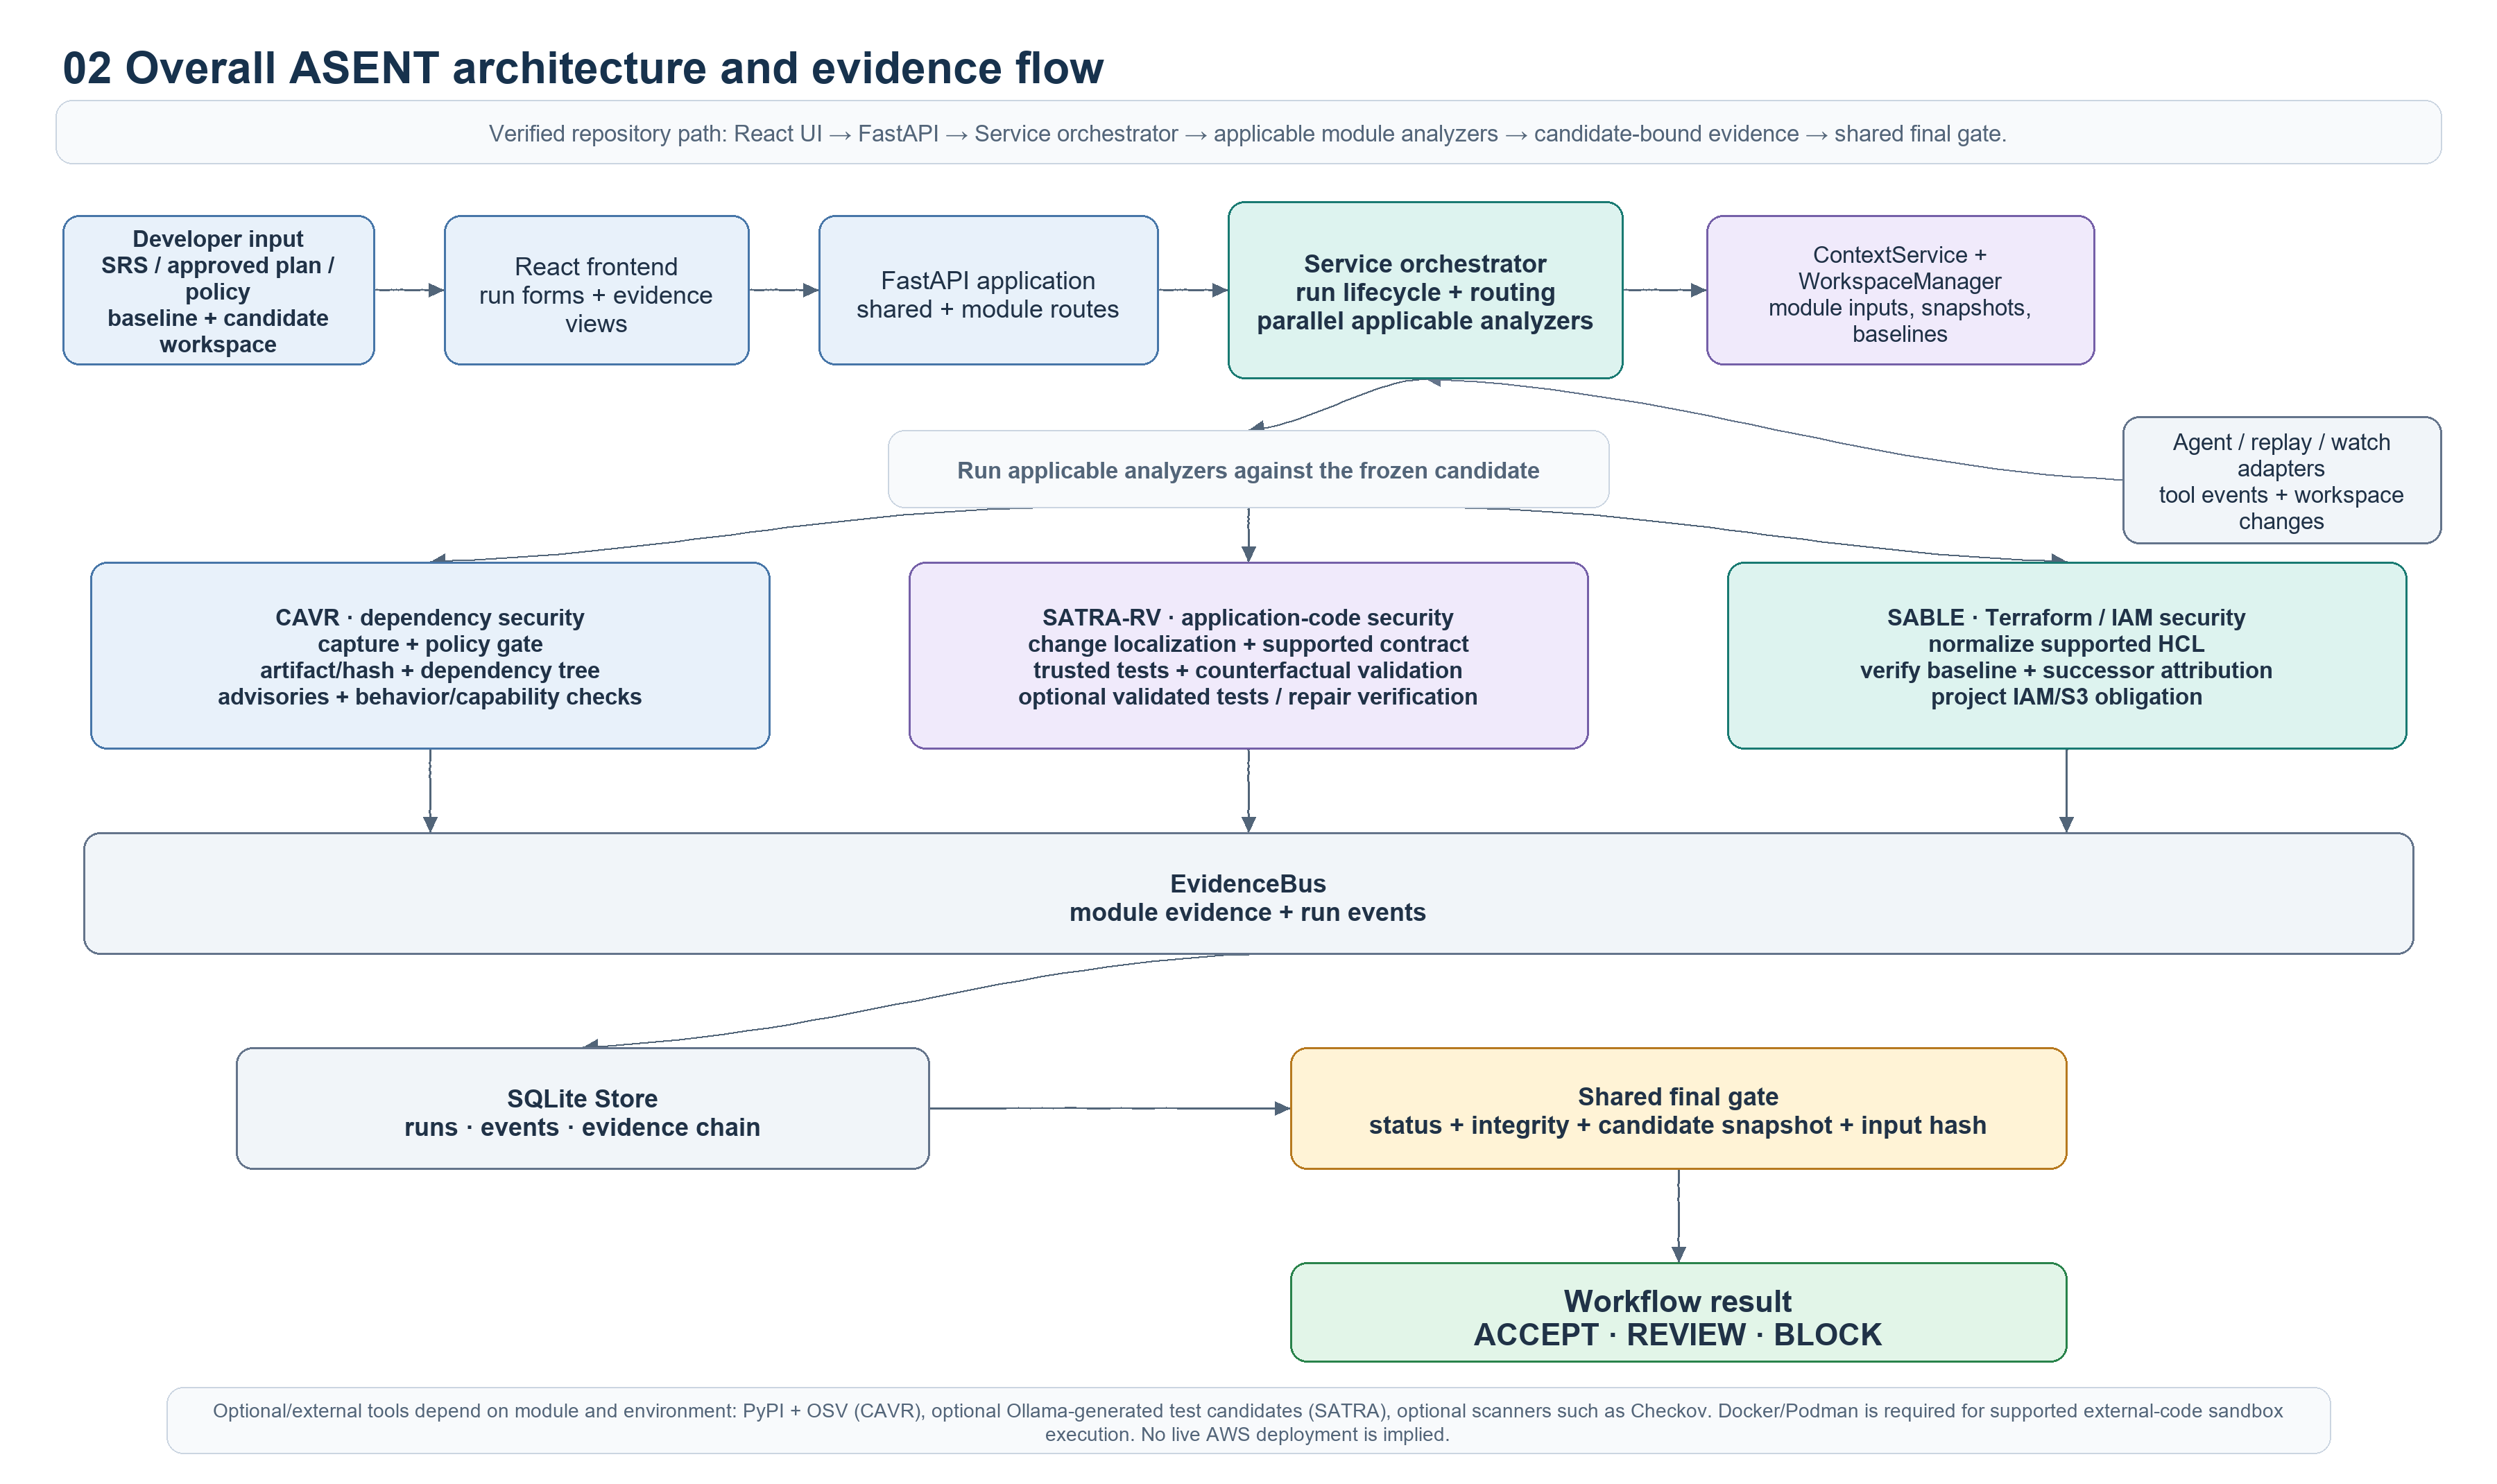
\includegraphics[width=0.97\linewidth,height=0.84\textheight,keepaspectratio]{figures/asent/asent-architecture.png}
\caption{Implemented ASENT architecture and evidence flow. Applicable analyzers publish module evidence through the local evidence bus/store; the shared final gate checks evidence bindings before returning an overall result. This is not a hosted deployment diagram.}
\label{fig:asent-overall-architecture}
\end{figure}
\end{landscape}

\section{Process and Shared Decision Design}
The SABLE behavior in Figure~\ref{fig:sable-current-process} is page 07 of the editable diagrams.net source. Its decision order is grounded in \path{backend/sable/analyzer.py}, \path{backend/sable/correspondence.py}, and the authorization evaluators: verify the trusted baseline obligation, rank candidate successors, and evaluate the same principal/action/resource scope against the selected successor. If the baseline, correspondence, binding, or authorization semantics are insufficient, the result remains \texttt{UNKNOWN}.

\begin{landscape}
\begin{figure}[p]
\centering
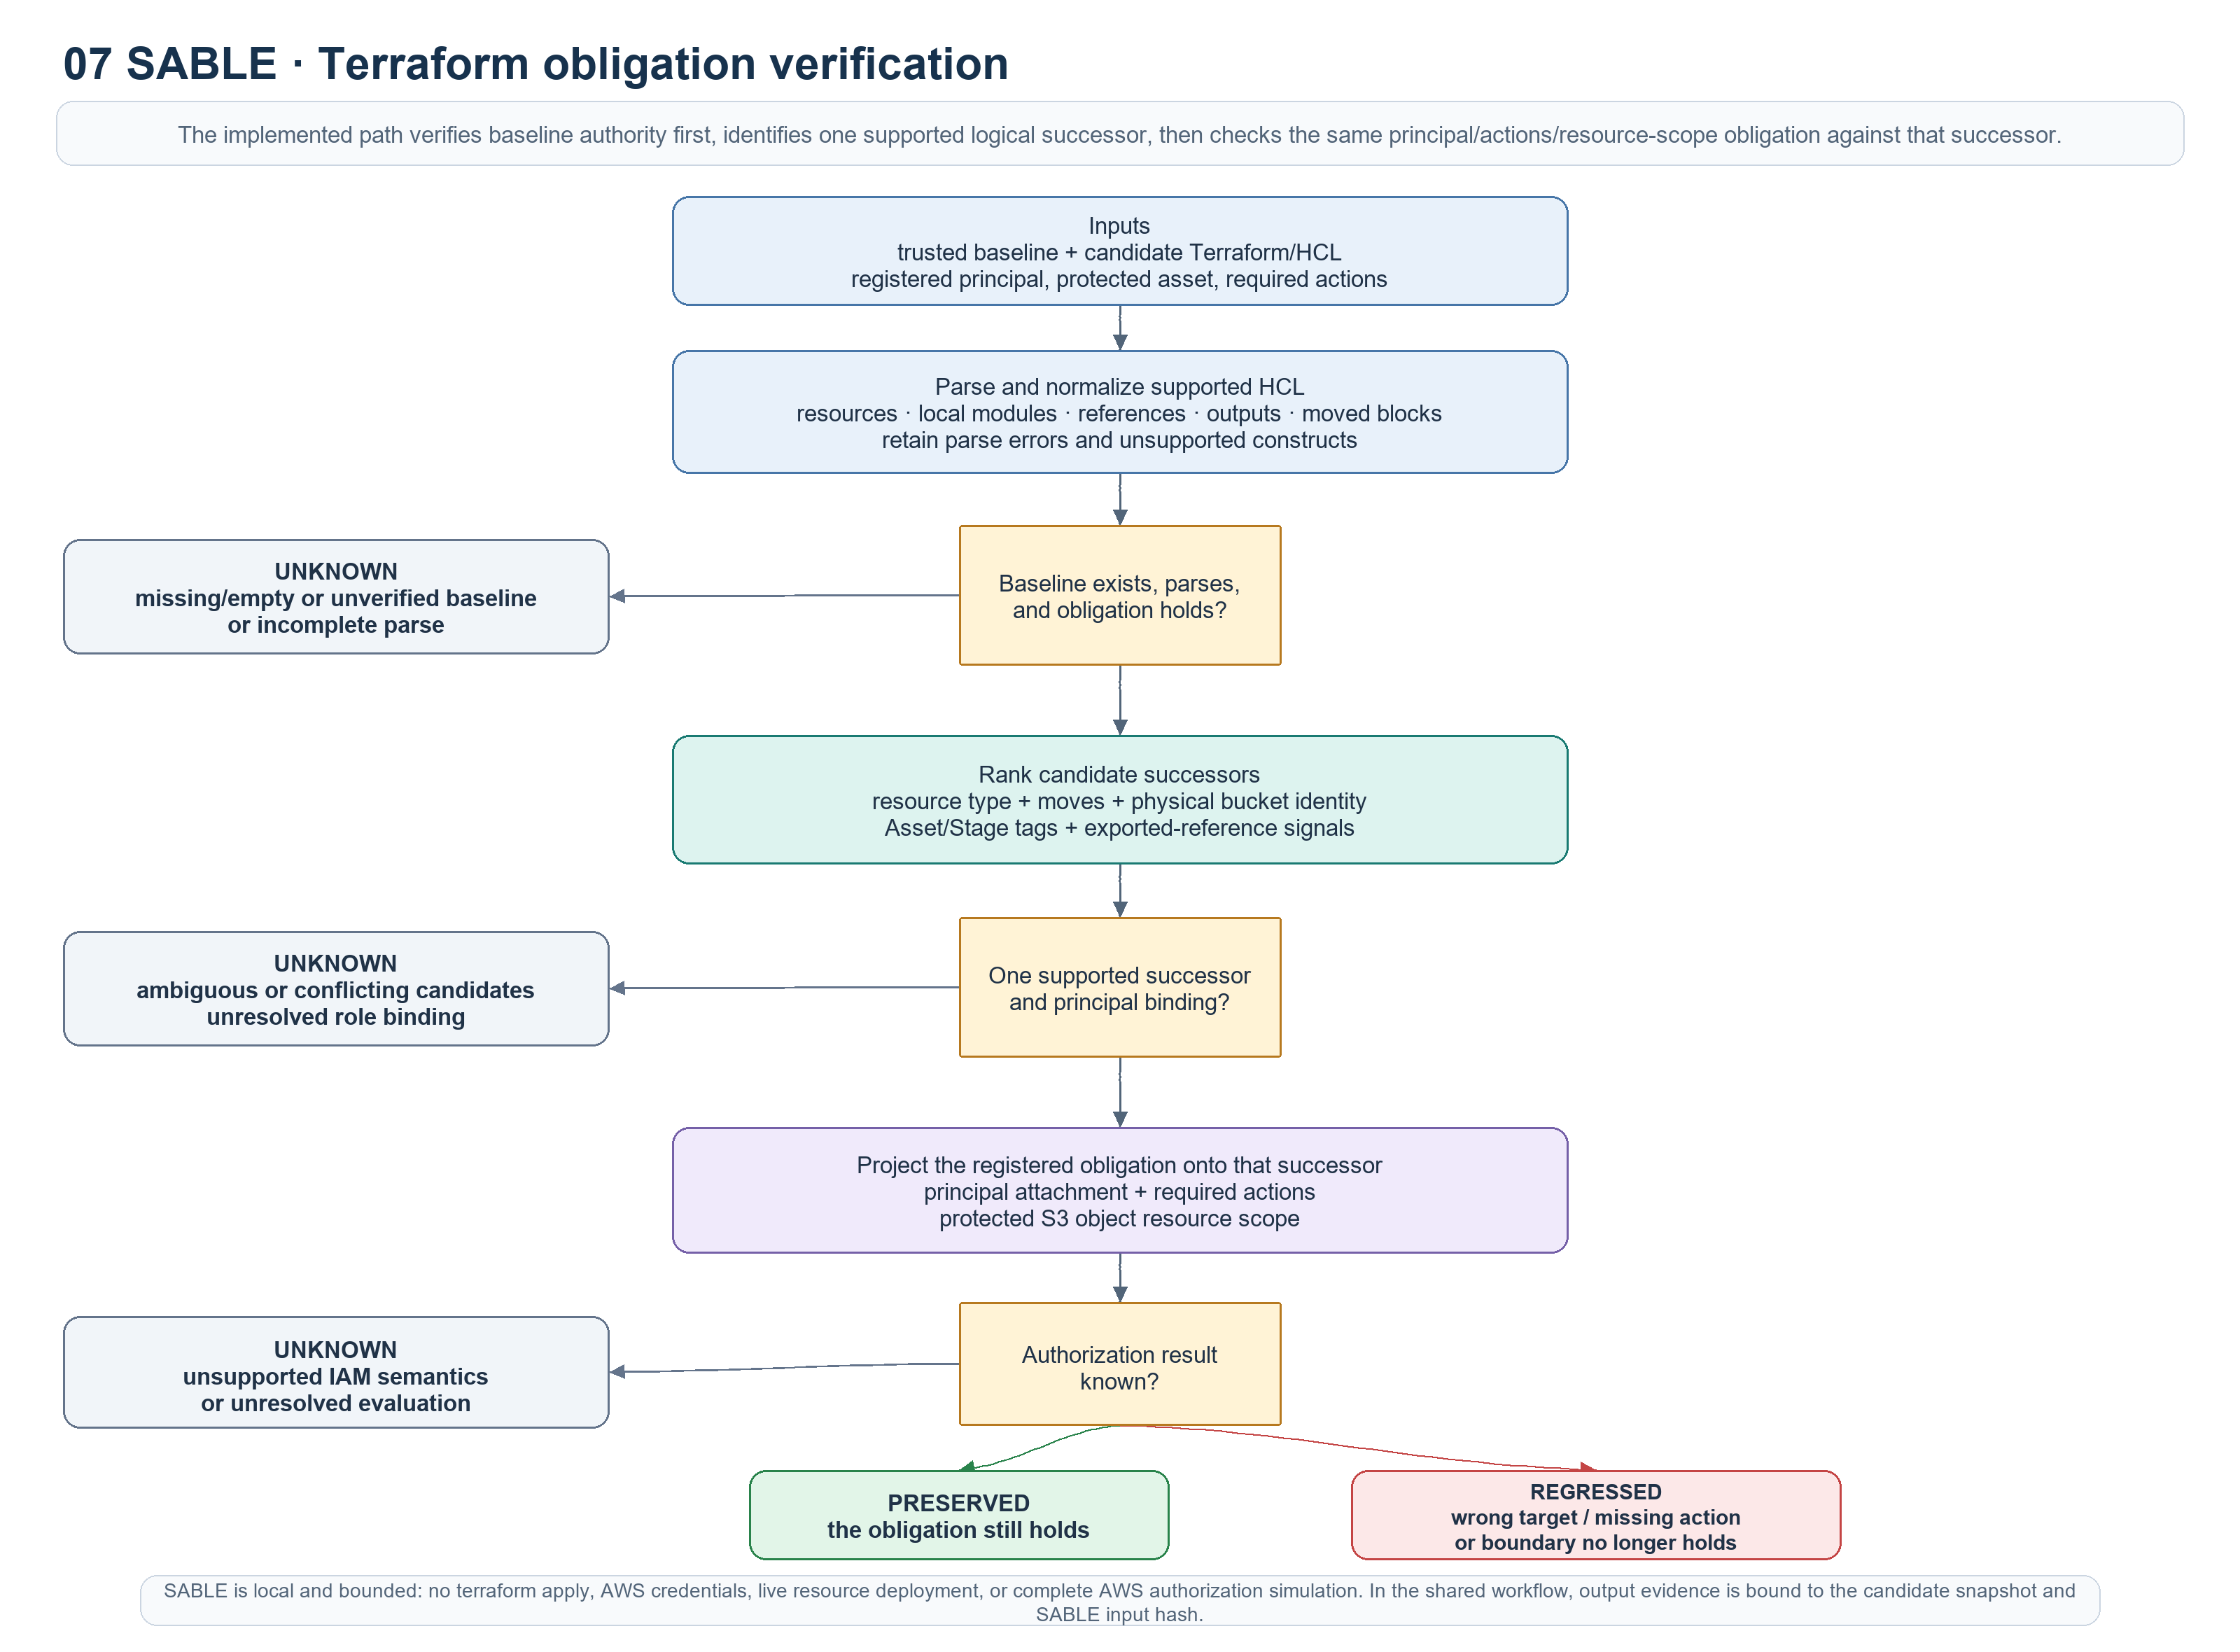
\includegraphics[width=0.97\linewidth,height=0.84\textheight,keepaspectratio]{figures/asent/sable-assurance-flow.png}
\caption{SABLE baseline-first Terraform obligation verification from page 07 of the editable diagrams.net source. No Terraform apply or live AWS authorization query is part of this path.}
\label{fig:sable-current-process}
\end{figure}
\end{landscape}

The shared final gate is a separate operation from the module verdict. Figure~\ref{fig:asent-shared-final-gate} is page 09 of the same editable source and shows how applicable CAVR, SATRA-RV, and SABLE statuses are combined only after evidence integrity, candidate snapshot, and input hashes are checked. A preserved SABLE result alone therefore does not imply an overall \texttt{ACCEPT}.

\begin{landscape}
\begin{figure}[p]
\centering
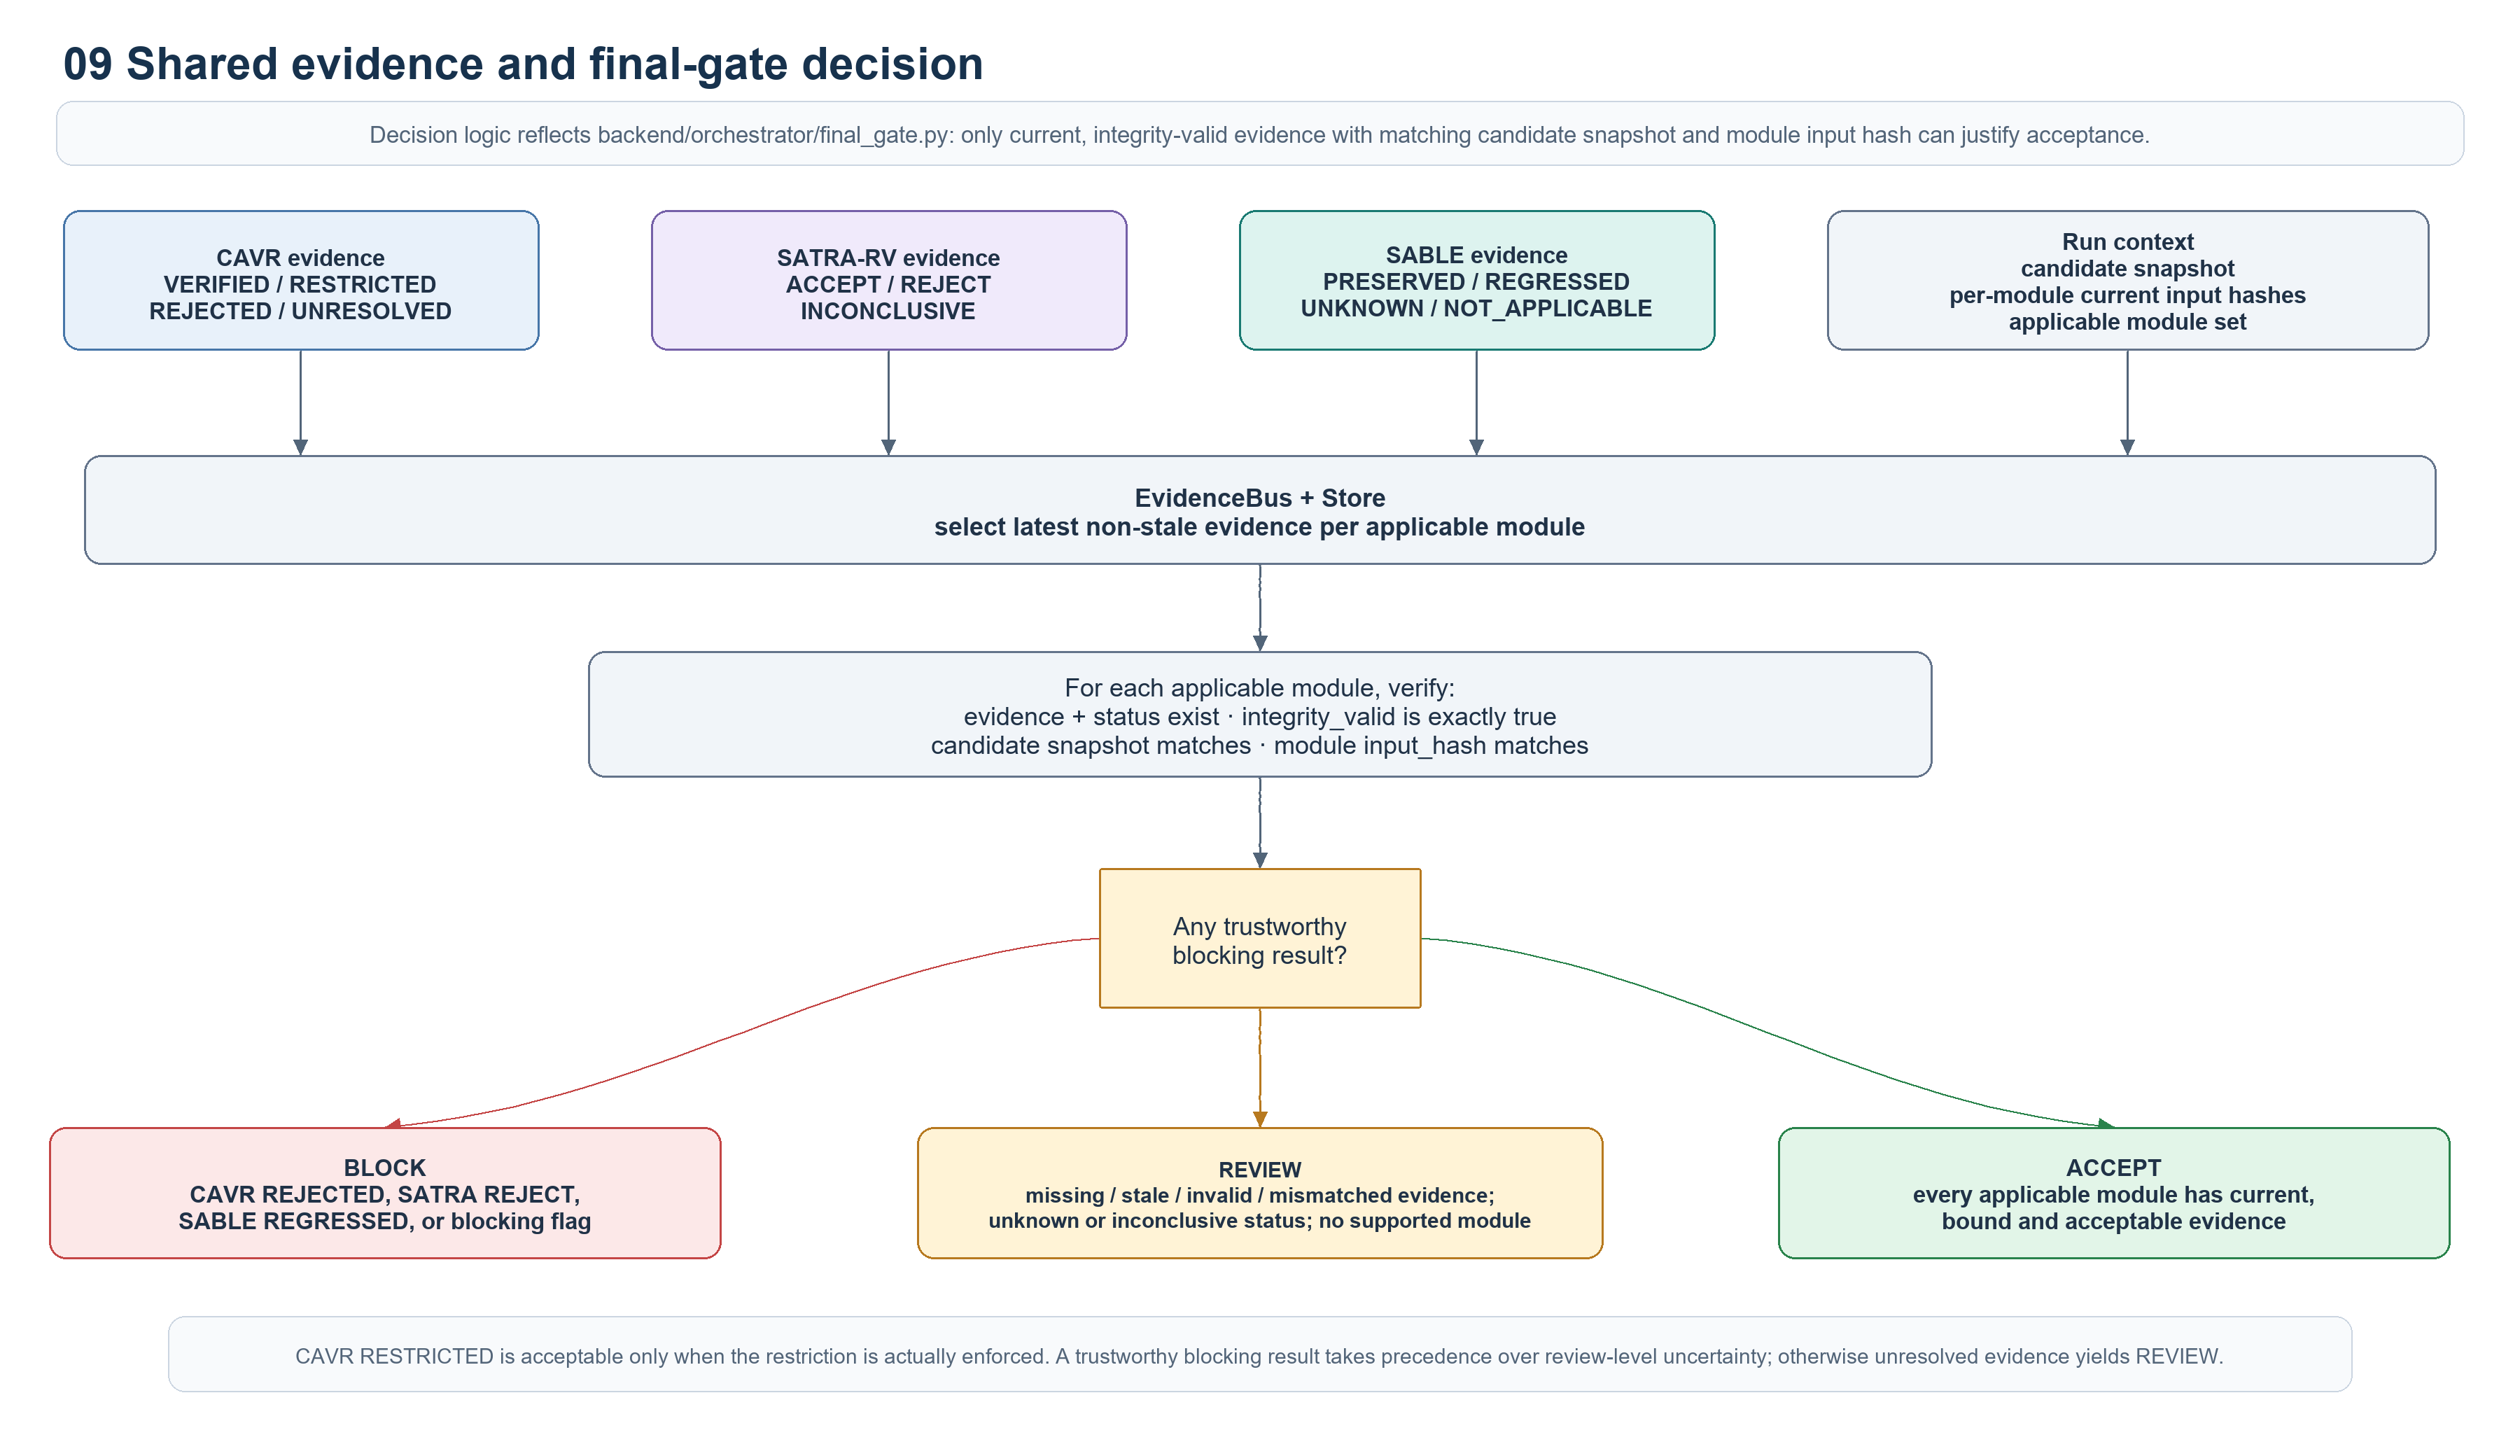
\includegraphics[width=0.97\linewidth,height=0.84\textheight,keepaspectratio]{figures/asent/shared-final-gate.png}
\caption{Shared final-gate outcomes from page 09 of the editable diagrams.net source. A trustworthy blocking status yields \texttt{BLOCK}; incomplete, stale, mismatched, invalid, or inconclusive evidence requires \texttt{REVIEW}; \texttt{ACCEPT} requires all applicable evidence to be acceptable.}
\label{fig:asent-shared-final-gate}
\end{figure}
\end{landscape}

CAVR \texttt{RESTRICTED} is accepted by the gate only when the restriction is enforced; no current CAVR path emits it.

\section{Architectural Components}
\begin{longtable}{p{0.27\textwidth}p{0.65\textwidth}}
\caption{Architectural Components -- supporting table 1}\\
\toprule
\textbf{Component} & \textbf{Implemented responsibility}\\
\midrule
\path{backend/sable/analyzer.py} & Coordinates the baseline check, candidate analysis, correspondence, authorization projection, scenario result, and evidence details.\\
\path{backend/sable/hcl_parser.py} & Parses the supported HCL input and normalizes resource records, references, local-module outputs, and moved-block data.\\
\path{backend/sable/correspondence.py} & Scores same-type candidate successors using address, move, physical bucket, tags, lifecycle, and exported-reference signals; rejects conflicting or insufficiently separated candidates.\\
\path{backend/sable/authorization.py} & Standalone SABLE evaluator for the bounded policy model, including principal attachment, actions, resource scope, denies, and unsupported/unresolved conditions.\\
\path{backend/sable/policy\_semantics.py} & Shared analysis evaluator for its supported inline role-policy subset; the regression suite compares required cases across the two evaluators.\\
\path{backend/orchestrator/service.py} & Runs applicable analyzers and publishes evidence for the shared workflow with candidate and input bindings.\\
\path{backend/orchestrator/final\_gate.py} & Validates current evidence and maps module statuses into the workflow decision; another module may independently cause review or block.\\
\bottomrule
\end{longtable}

\section{Interfaces and Dependencies}
SABLE consumes baseline and candidate workspaces plus the registered obligation through the module context and API. HCL parsing uses \texttt{python-hcl2}; the resource-reference graph uses NetworkX. The service/API layer uses FastAPI and Pydantic. In the integrated route, the orchestrator stores SABLE evidence and the final gate consumes it. This report's tested shared route is exercised by \path{test_shared_sable_evidence_drives_final_gate}; the standalone SABLE UI and API are distinct entry points.

\section{Architecture Decisions and Rationale}
The central decision is to separate authorization validity from logical-asset correspondence. A policy may allow the required actions against a bucket and still fail the registered obligation if that bucket is not the protected successor. The system therefore verifies the trusted baseline, establishes a supported successor, then checks authorization on that successor. This order directly addresses the wrong-target fixture and prevents a candidate-local allow from being treated as proof of continuity.

Uncertainty is a first-class result. The successor selector abstains on ambiguity or conflicting signals, and unsupported or unresolved policy semantics remain unknown. The shared final gate independently checks evidence freshness, input binding, and integrity. This bounded design makes the evidence path inspectable without claiming arbitrary Terraform equivalence or complete AWS semantics.

\section{Design Evolution}
The implemented design retains B0--B4 analysis configurations for the planned comparison described in the SABLE research design. This is not evidence that a comparative research experiment has been completed. A focused correctness audit found a difference between the standalone and shared authorization evaluators for unresolved role attachment: the shared path returned unknown while standalone analysis ignored a dynamic binding. The standalone evaluator now marks unresolved bindings outside its model, while retaining the behavior that a statically known unrelated role can be ignored. Tests \path{test_sable_standalone_evaluator_fails_closed_on_unresolved_role_binding} and \path{test_sable_explicitly_unrelated_role_binding_is_ignored} cover both sides. The correction was committed as \texttt{58b0a3d}. A later gate audit corrected missing/empty baselines to SABLE \texttt{UNKNOWN}, makes SABLE \texttt{NOT\_APPLICABLE} yield final \texttt{REVIEW}, and requires integrity to be explicitly true with matching candidate and module-input bindings. These corrections are covered by tests and are present in source commit \texttt{84f91a9}, which is part of the integrated PR~\#5 change. The exact tested PR head was \texttt{554b6d51}; all 18 check runs succeeded before it was merged as \texttt{ffe8aa91}. The original 44-test CI run predates the unresolved-binding and later gate corrections; Chapter 7 separates all result provenance.

\section{Domain Model}
The principal domain objects are the trusted baseline obligation (identifier, principal, protected asset, required actions and scope), normalized Terraform resources and references, successor hypotheses with evidence signals, authorization evaluation, candidate-bound module evidence, and the shared decision. The obligation under the acceptance tests is \texttt{S3-APPROLE-CUSTOMERDATA}.

The editable diagrams.net source page 08 separates the registered obligation, baseline and candidate resource models, successor hypothesis, authorization projection, module result, bound evidence, and shared final decision. Figure~\ref{fig:sable-domain-model} uses that source page directly; correspondence and authorization are shown as distinct operations because the implementation first chooses a supported successor and then checks the obligation on it.

\begin{landscape}
\begin{figure}[p]
\centering
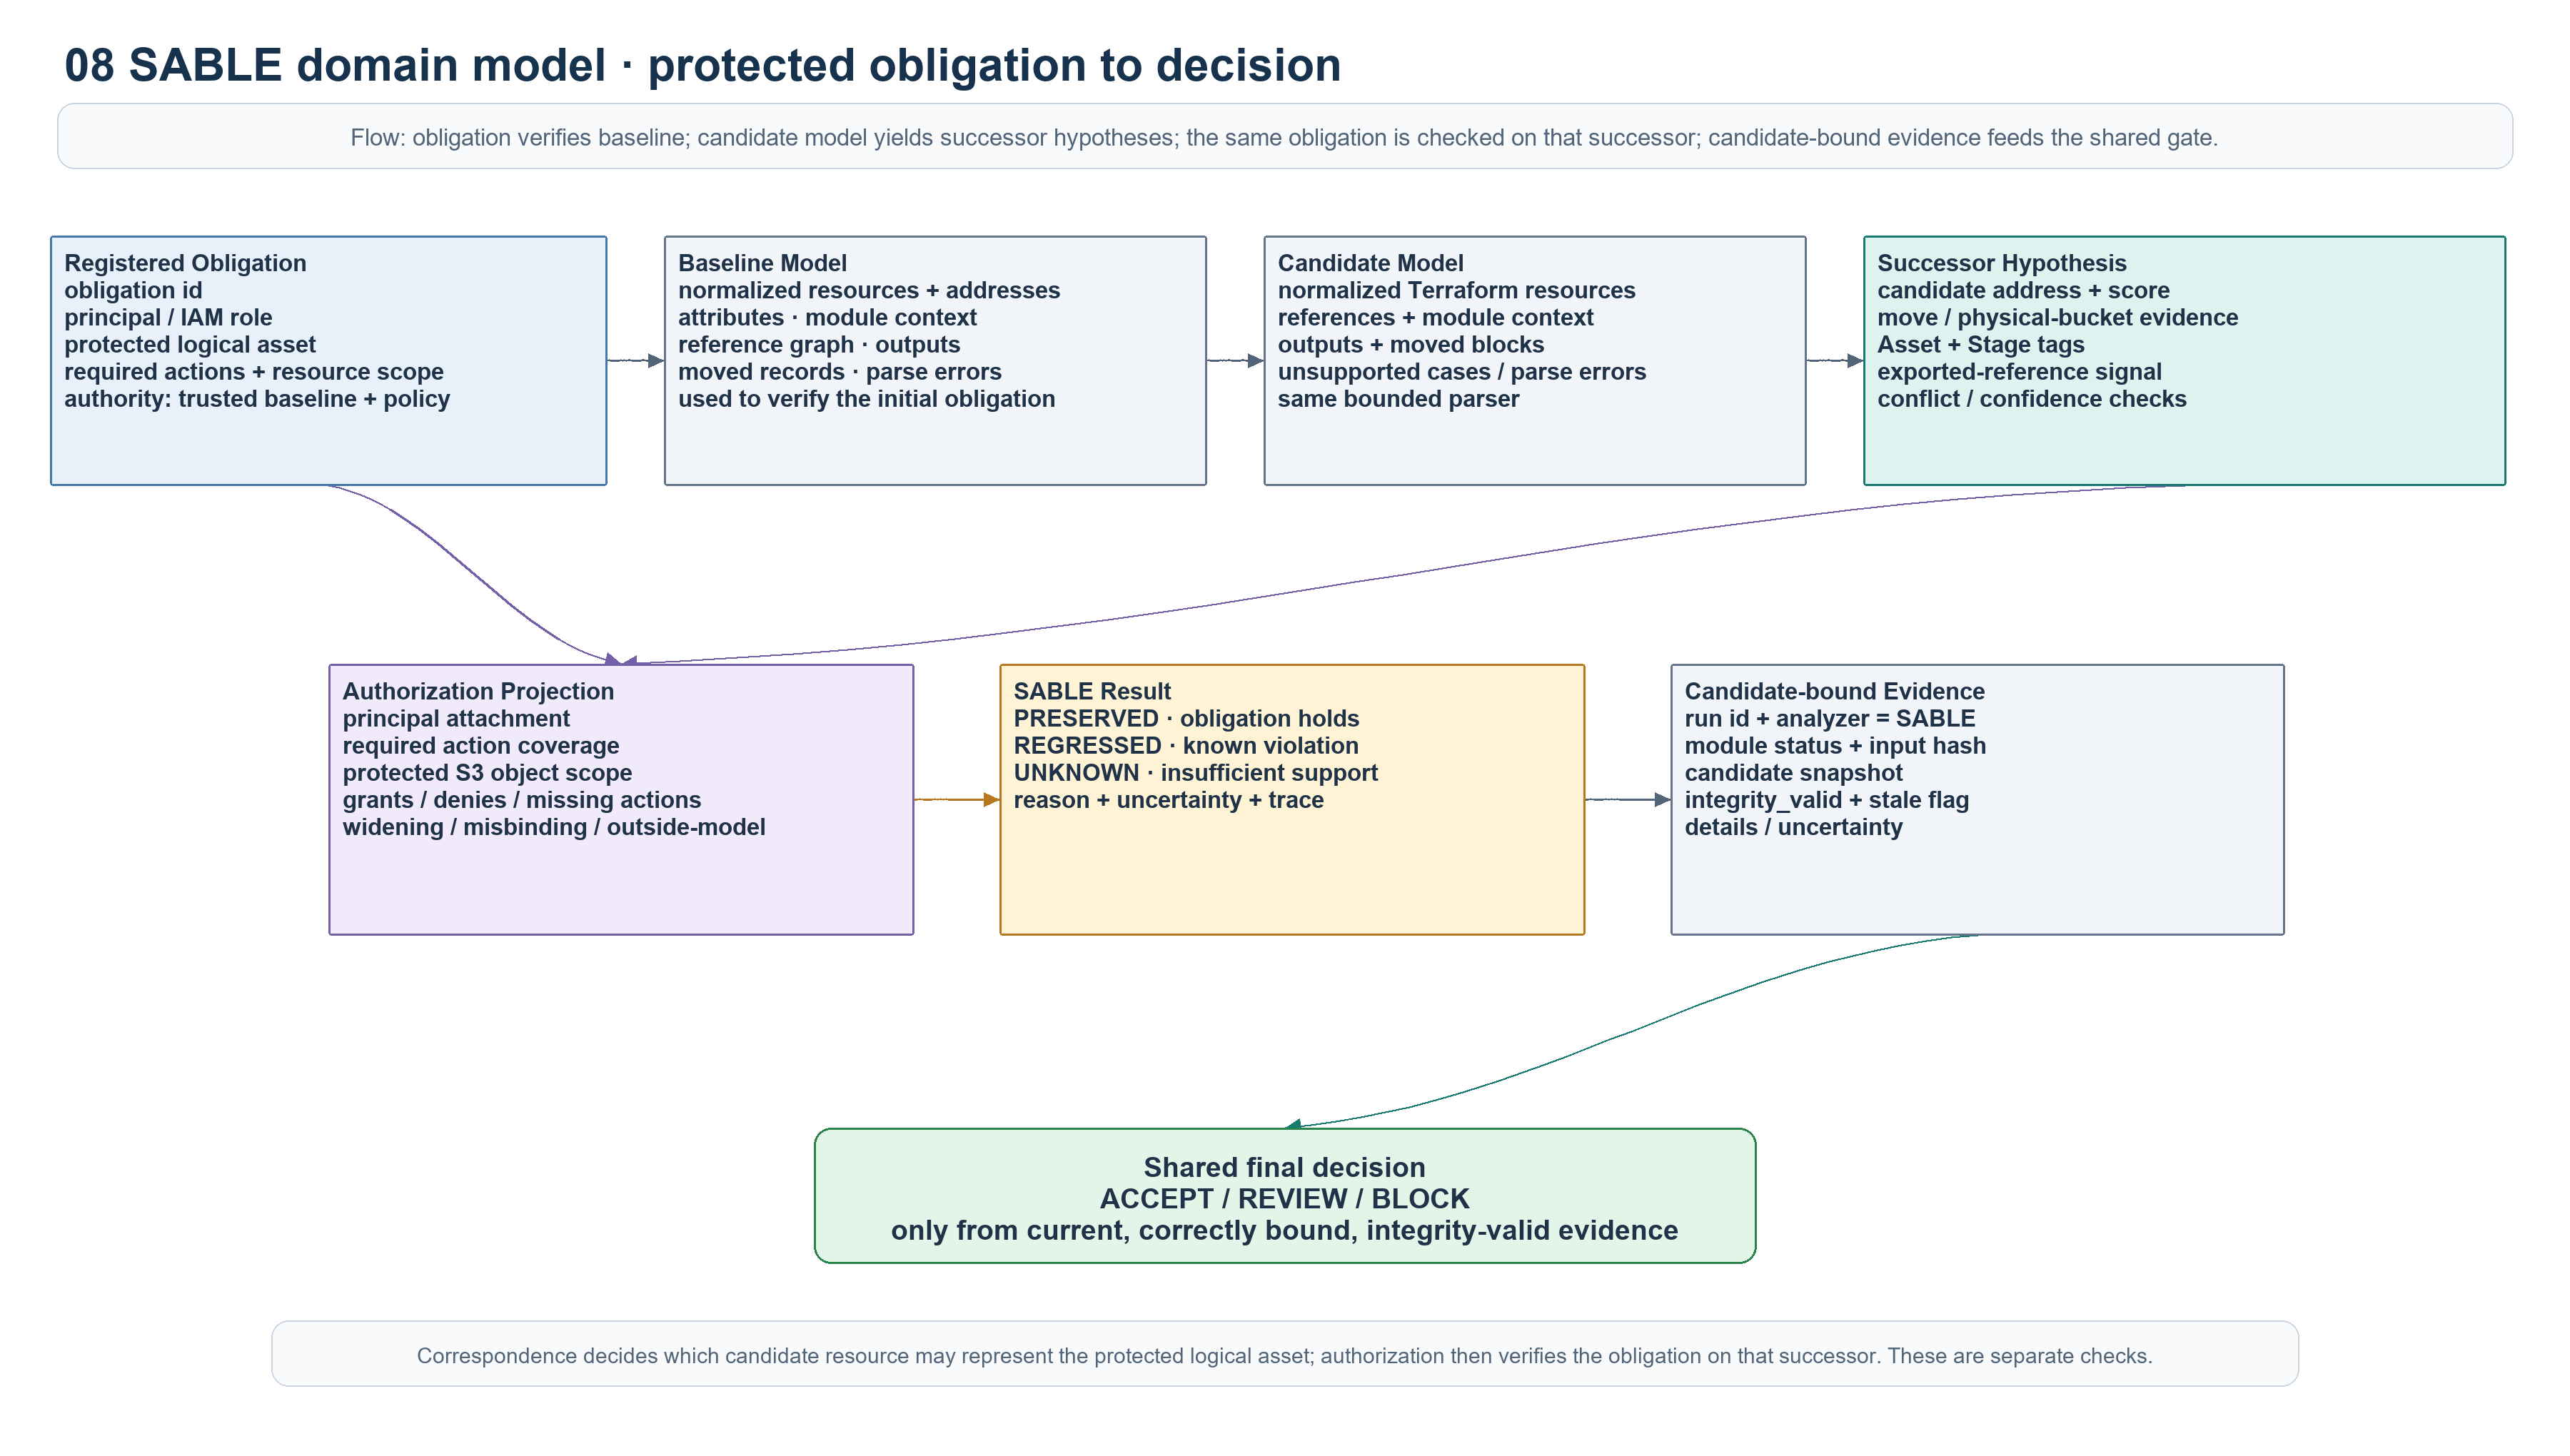
\includegraphics[width=0.97\linewidth,height=0.84\textheight,keepaspectratio]{figures/asent/sable-domain-model.png}
\caption{SABLE domain model from page 08 of the editable diagrams.net source. Evidence is eligible for the shared decision only when it is current, candidate-bound, integrity-valid, and matched to the module input.}
\label{fig:sable-domain-model}
\end{figure}
\end{landscape}

\section{Data Design}
\begin{figure}[htbp]
\centering
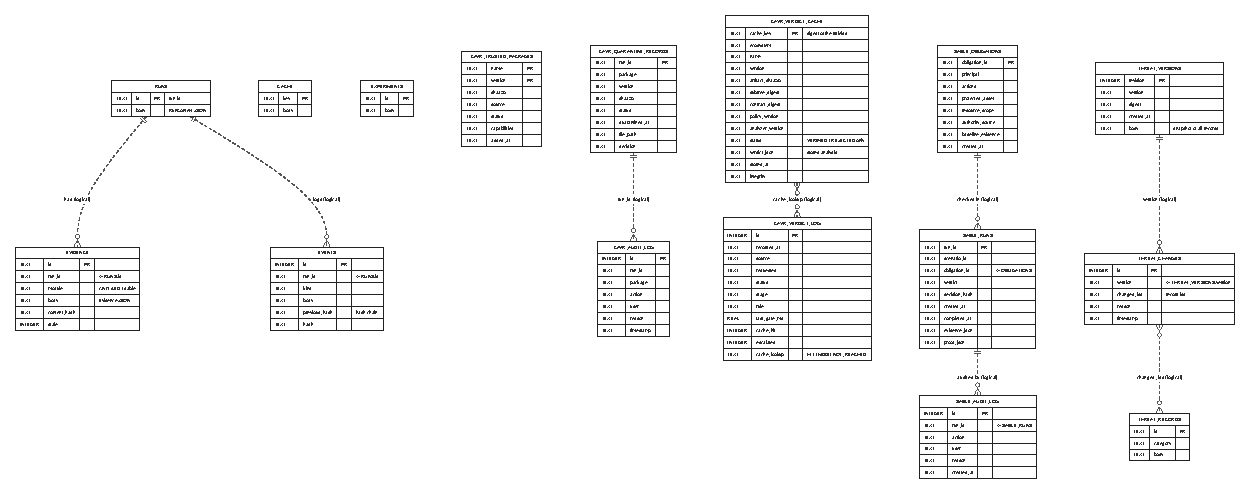
\includegraphics[width=\textwidth]{figures/diagrams/erd.pdf}
\caption{Entity--relationship diagram of the SQLite stores (\texttt{db/storage.py}, \texttt{cavr/storage.py}, \texttt{sable/storage.py}, \texttt{threat\_repo/repository.py}). Dashed relationships are logical: the code writes the same identifier into both tables but declares no foreign keys.}
\label{fig:asent-erd}
\end{figure}

Figure~\ref{fig:asent-erd} shows the persistent data. The shared run store keeps each run as a \texttt{RunContext} JSON document, the module evidence bound to it (with a content hash and a stale flag) and the run events as a hash chain. The CAVR store holds the M1 \texttt{verdict\_cache}, keyed by a digest of the eight key fields and storing only complete analyses with an integrity value, and the \texttt{verdict\_log}, one row per request, from which the cache hit rate and the p50/p95 latency are computed; the trusted-package, quarantine and audit tables come from the earlier prototype. The SABLE store holds registered obligations, SABLE runs and their audit log, and the threat repository versions its records so that every change has a version and a reason. Integrity is enforced by the code (shared identifiers, content hashes, hash chains) rather than by declared foreign keys.

The parser's normalized resource model carries Terraform address, type, attributes, module context, and graph references. Correspondence returns ranked hypotheses and conflict reasons. Authorization results contain known/holds values, expected and unexpected resources, missing actions, widening, misbinding, and outside-model evidence. The orchestrator evidence includes run identity, analyzer, candidate snapshot, input hash, status, stale state, and integrity result. The gate uses these fields to decide whether evidence is current and trustworthy.

\section{Process / Behavior Design}
The sequence in Figure~\ref{fig:sable-current-process} is fail-closed at decision boundaries: a missing, empty, or unverified baseline cannot establish continuity; no unique supported successor means no projected safe result; unsupported policy meaning cannot prove the obligation; SABLE \texttt{NOT\_APPLICABLE} and stale, mismatched, or integrity-invalid evidence cannot establish acceptance. The shared gate requires \texttt{integrity\_valid} to be exactly true and checks candidate-snapshot and module-input-hash bindings. Tests exercise these conditions and map unknown or not-applicable SABLE evidence to final \texttt{REVIEW}.

\begin{figure}[htbp]
\centering
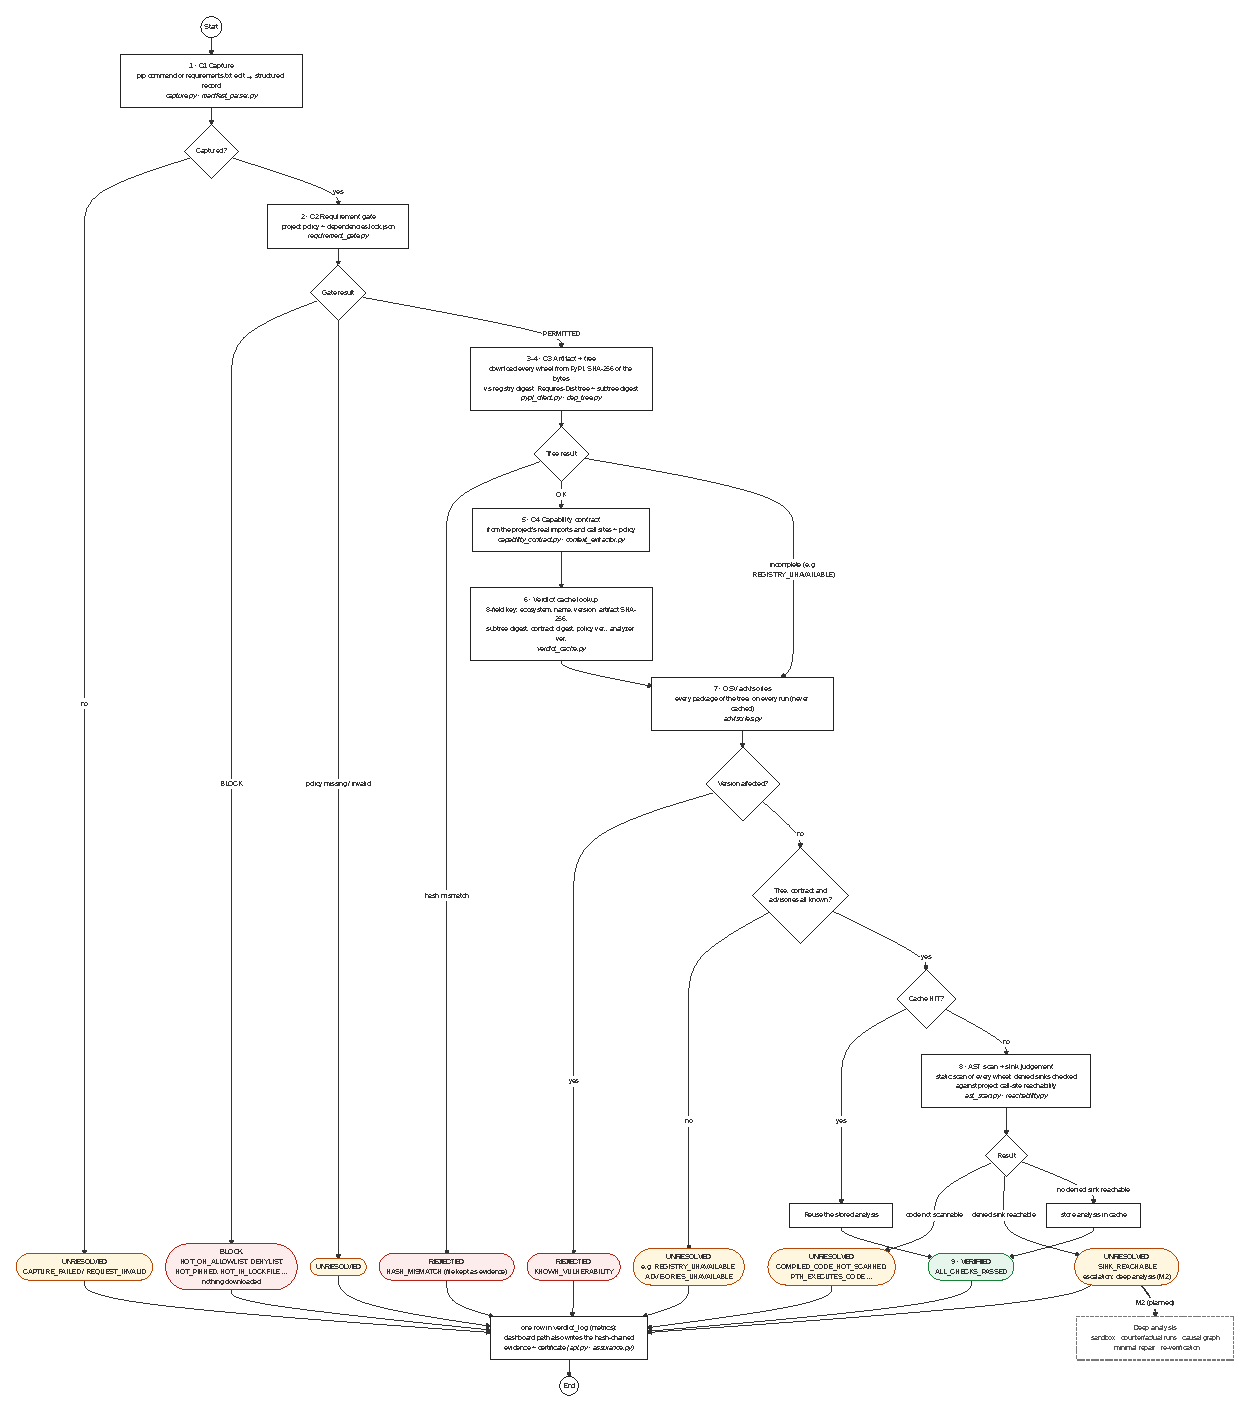
\includegraphics[height=0.88\textheight]{figures/diagrams/cavr-activity.pdf}
\caption{Activity diagram of the CAVR fast gate, \texttt{verify\_request} in \texttt{backend/cavr/pipeline.py}. Numbers follow the stage order in the code; the dashed element is planned (M2).}
\label{fig:cavr-activity}
\end{figure}

Figure~\ref{fig:cavr-activity} follows \texttt{verify\_request} stage by stage. The request is captured as a structured record (1) and checked by the requirement gate against the project policy and the lockfile (2); a request that is not permitted ends as \texttt{BLOCK} before anything is downloaded. Every wheel of the dependency tree is then downloaded from PyPI and its SHA-256 compared with the registry digest, and the tree and its subtree digest are built from the real \texttt{Requires-Dist} metadata (3--4); a mismatch is \texttt{REJECTED}. The capability contract is inferred from the project's own imports and call sites (5); only then can the 8-field cache key be formed and looked up (6), because it contains the contract digest. OSV is asked for every package of the tree on every run, also on a cache hit (7): an affected version is \texttt{REJECTED}, and any unknown input (registry, contract or advisories) is \texttt{UNRESOLVED}. On a cache miss the wheels are scanned statically and every denied sink is judged against the project's call-site reachability (8). A reachable denied sink is not treated as proven malicious: the verdict is \texttt{UNRESOLVED} with an escalation to M2 deep analysis. Only a complete analysis is stored in the cache. Every verdict writes one row to the verdict log; requests made from the dashboard also write the hash-chained evidence and the certificate.

\begin{figure}[htbp]
\centering
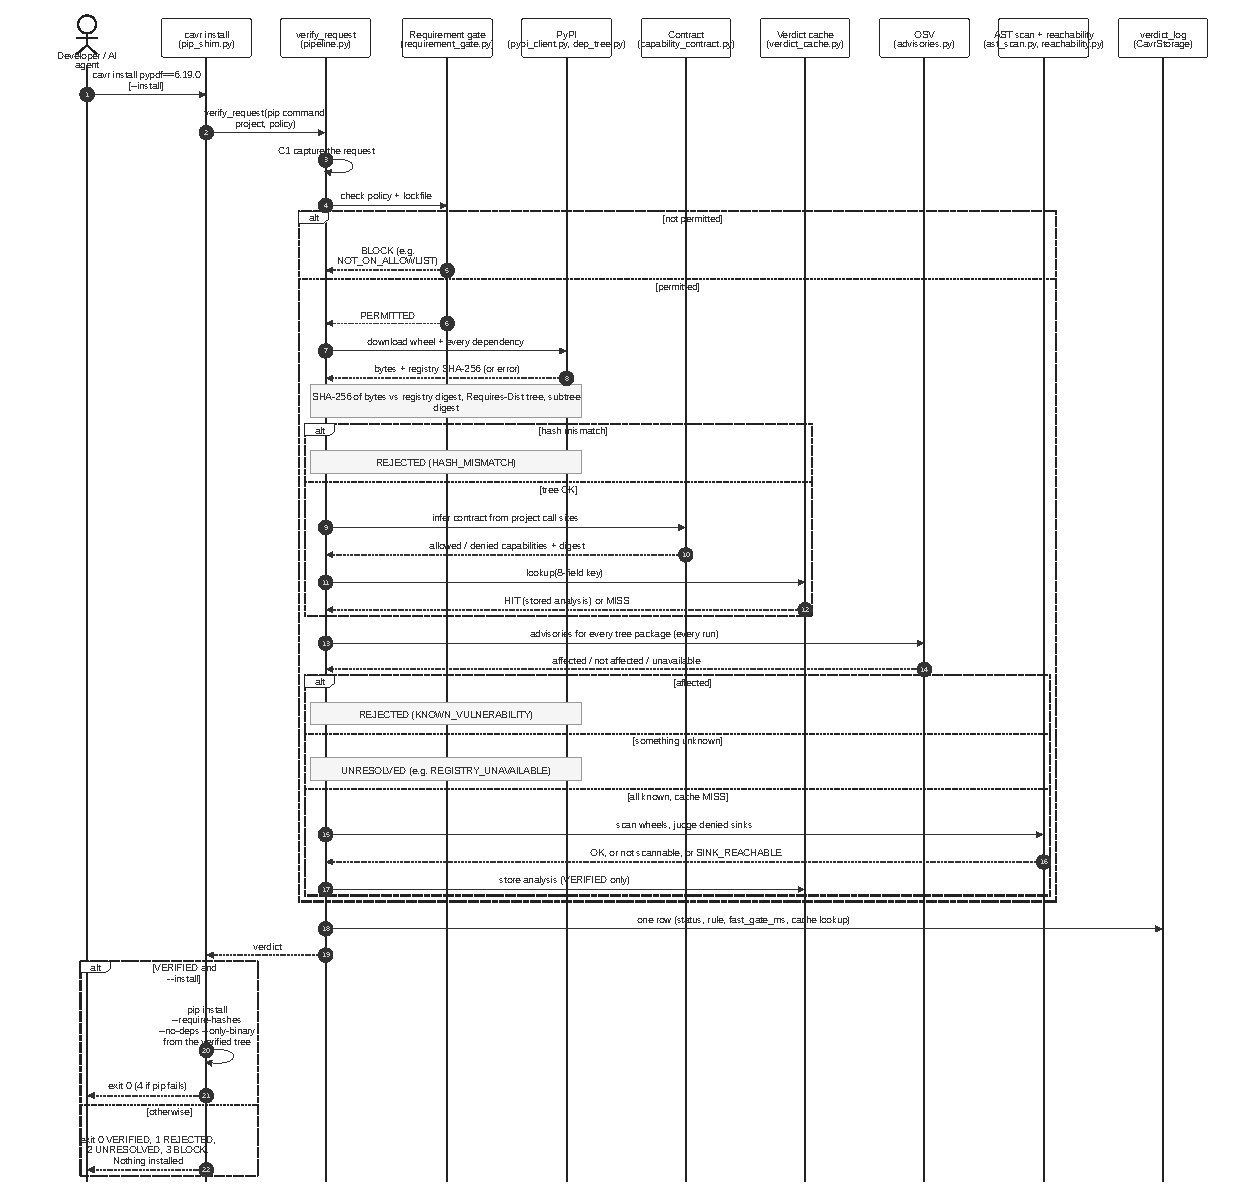
\includegraphics[width=\textwidth]{figures/diagrams/cavr-sequence.pdf}
\caption{Sequence of a \texttt{cavr install} request (\texttt{pip\_shim.py}) through \texttt{verify\_request} and its collaborators, with the wrapper's exit codes.}
\label{fig:cavr-sequence}
\end{figure}

Figure~\ref{fig:cavr-sequence} shows the same pipeline as messages between components. The wrapper never passes the user's arguments to pip; it only calls \texttt{verify\_request} and prints the verdict (exit code 0 \texttt{VERIFIED}, 1 \texttt{REJECTED}, 2 \texttt{UNRESOLVED}, 3 \texttt{BLOCK}). Only with \texttt{--install} and a \texttt{VERIFIED} verdict does it write a requirements file of the verified tree with \texttt{--hash=sha256} pins and run pip with \texttt{--require-hashes --no-deps --only-binary :all:}, so pip cannot install a different file, an unverified dependency or an sdist; a pip failure gives exit code 4.

\begin{figure}[htbp]
\centering
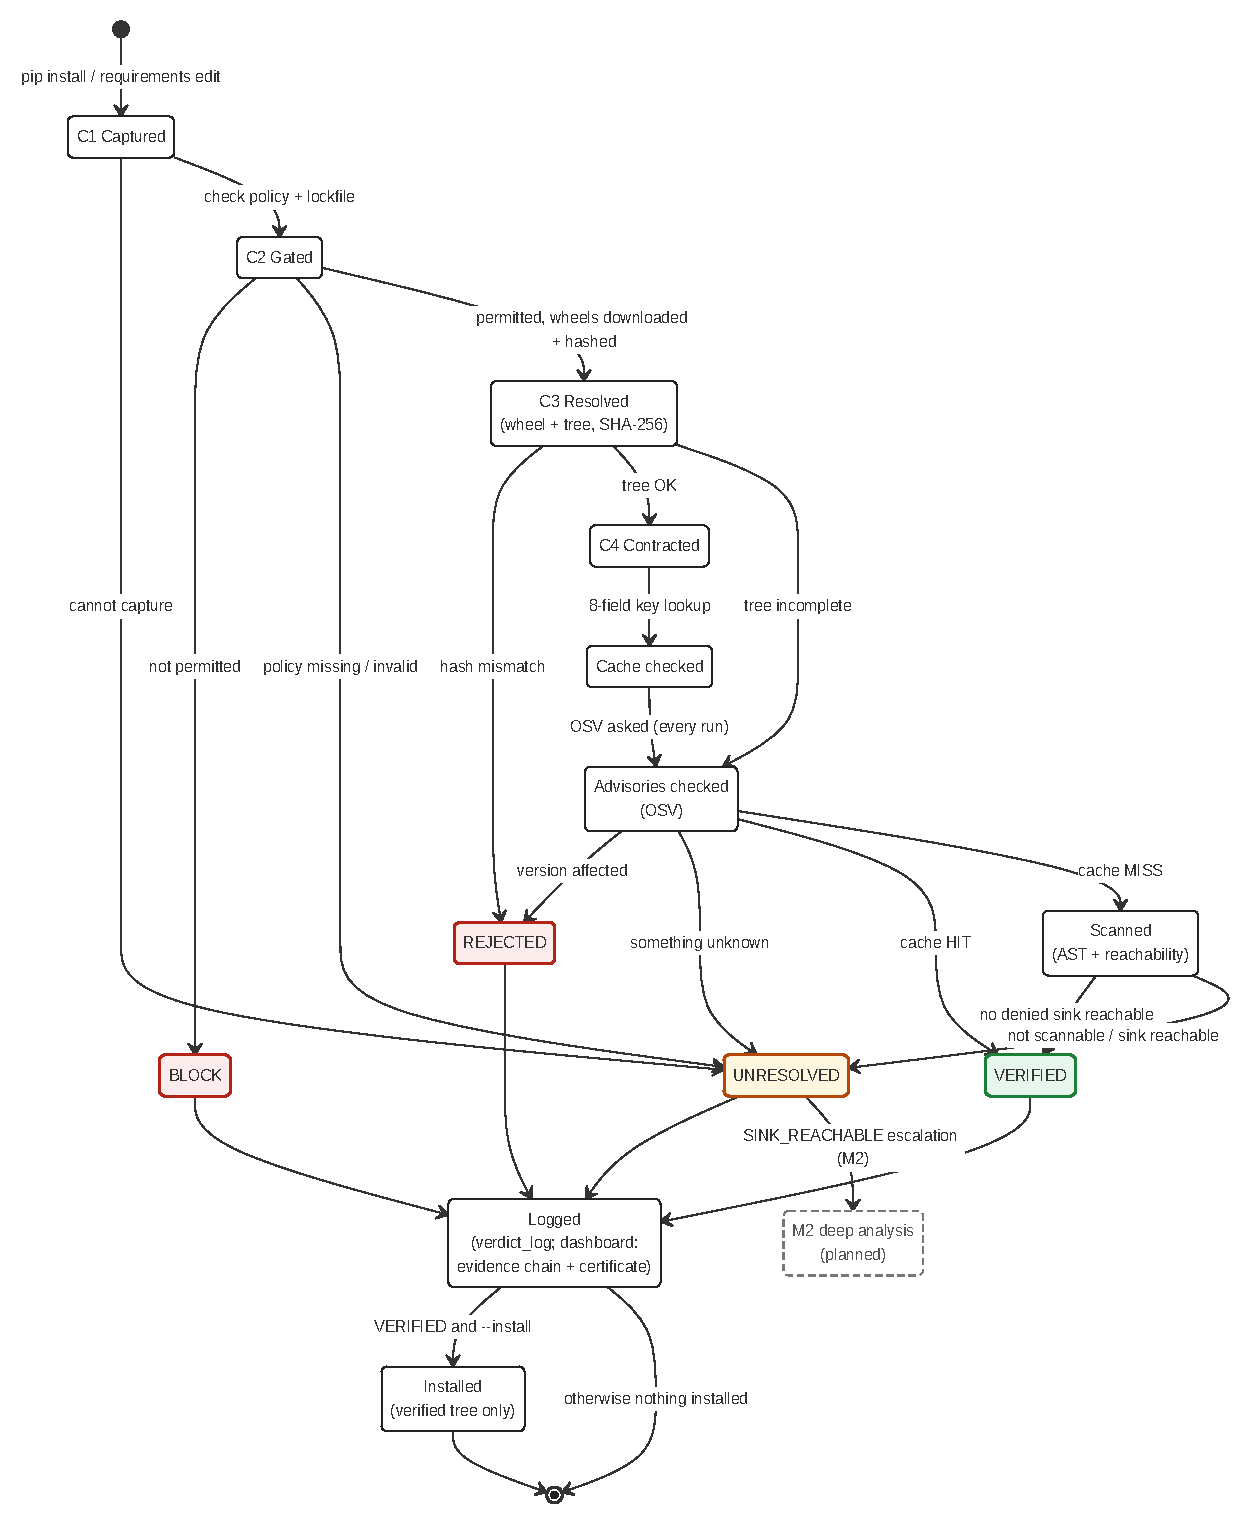
\includegraphics[width=0.85\textwidth]{figures/diagrams/cavr-state.pdf}
\caption{Lifecycle of a CAVR request. All four verdicts are logged; only a \texttt{VERIFIED} request with \texttt{--install} is installed.}
\label{fig:cavr-state}
\end{figure}

Figure~\ref{fig:cavr-state} shows the states of one request. \texttt{REJECTED} is reached only with positive evidence of a problem (a hash mismatch or an OSV advisory); every gap in the evidence leads to \texttt{UNRESOLVED}, which is never treated as a pass. \texttt{UNRESOLVED} with \texttt{SINK\_REACHABLE} is the state that M2 deep analysis will take over.

\chapter{Iteration 1: Design and Implementation}

This chapter records the implementation that can be tied to the current repository evidence, with emphasis on SABLE and its connection to the shared ASENT assurance workflow. It separates working mechanisms from planned work and does not treat a static analysis result as proof that infrastructure was deployed or tested against a live cloud account.

\section{Iteration Objectives}

The iteration objective was to implement a reproducible infrastructure-security check for Terraform changes and connect its result to ASENT's shared evidence and decision path. SABLE addresses a specific continuity problem: after an infrastructure refactor, the resource that now represents a protected logical asset may not be the resource that looks most similar by name. A policy can still be syntactically valid while granting access to the wrong bucket or granting broader access than the registered obligation permits.

The implementation therefore aims to:
\begin{itemize}
    \item parse a trusted Terraform baseline and a candidate version into comparable resource models;
    \item check a registered principal, protected asset, and required action set against the baseline before making a continuity claim;
    \item identify a candidate successor using explicit move information and structural evidence, and abstain when evidence is ambiguous;
    \item evaluate the supported IAM/S3 policy subset on the selected successor; and
    \item emit a traceable result that the shared ASENT gate can accept, block, or send for review.
\end{itemize}

\section{Selected Use Cases / Features}

The implementation focuses on the following use cases.

\begin{enumerate}
    \item \textbf{Check a refactor that preserves an obligation.} The resource address may change, but the successor still satisfies the registered access requirement.
    \item \textbf{Detect a wrong-target or weakened policy.} A policy may continue to allow the required actions but point to a different bucket, or it may grant extra permissions. The target-to-obligation relationship must be checked as well as the policy syntax.
    \item \textbf{Handle ambiguous or unsupported changes conservatively.} Ambiguous moves, unsupported constructs, and incomplete evidence lead to \texttt{UNKNOWN}.
    \item \textbf{Carry module evidence into the shared gate.} Evidence is associated with the exact candidate snapshot and module input hash; stale or invalid evidence cannot silently authorize a new candidate.
\end{enumerate}

\section{Design}

SABLE uses a bounded, local analysis pipeline. The baseline is an authority supplied by prior approval; SABLE does not decide that an arbitrary baseline is trustworthy. For the current S3 obligation, the registered principal is the application IAM role, the protected asset is the customer-data bucket, and the required actions are \texttt{s3:GetObject} and \texttt{s3:PutObject} on the bucket's object scope.

The pipeline follows these steps:
\begin{enumerate}
    \item \textbf{Load evidence and parse both snapshots.} Terraform files are normalized into resource records, references, module outputs, move records, and a resource-reference graph.
    \item \textbf{Validate the baseline.} The required authorization predicate must be known and hold on the trusted baseline before continuity is assessed.
    \item \textbf{Find a candidate successor.} SABLE scores resource-type and structural signals, including unchanged address, explicit \texttt{moved} blocks, physical bucket identity, stable asset/lifecycle tags, and preserved references. A unique candidate must meet the configured confidence threshold and margin; conflicts or close scores result in abstention.
    \item \textbf{Project the obligation.} The required principal and actions are evaluated against the selected successor. The existence of some policy grant is not enough if it is attached to the wrong logical asset.
    \item \textbf{Emit the verdict and evidence.} The analysis returns \texttt{PRESERVED}, \texttt{REGRESSED}, or \texttt{UNKNOWN} for the supported continuity cases, along with reasons and evidence details. The shared gate checks the current snapshot, input hash, and evidence integrity before making a workflow-level decision.
\end{enumerate}

\section{Implementation}

The SABLE implementation is in the \texttt{backend/sable/} package. Its HCL parser reads local Terraform files and builds a resource graph. The authorization evaluator interprets a bounded IAM/S3 subset. The correspondence logic proposes successors from structural and reference signals rather than resource-name similarity alone. The API exposes scenario runs, progress events, run results, proof/evidence inspection, audit actions, and a benchmark endpoint.

The shared workflow is implemented through the orchestrator and its front-end Run Workflow view. The final gate evaluates module statuses against the same candidate snapshot and expected module input hashes. Current, integrity-valid \texttt{PRESERVED} or module-level \texttt{NOT\_APPLICABLE} evidence is acceptable. \texttt{REGRESSED} blocks. \texttt{UNKNOWN}, missing evidence, stale evidence, or failed integrity requires review unless another result already blocks.

\section{Completed Features / Module}

The verified integrated snapshot contains the following SABLE features:
\begin{itemize}
    \item parsing and normalization of supported Terraform resources, local modules, resource references, outputs, and \texttt{moved} blocks;
    \item a bounded authorization check for relevant IAM role policies and bucket policies, including required actions and resource scope;
    \item resource-successor ranking and ambiguity handling;
    \item explicit handling for invalid baselines, parse errors, unresolved bindings, and unsupported constructs;
    \item baseline variants B0--B4 for comparing candidate-only policy checks, before/after checks, move evidence, structural correspondence, and the combined obligation-projection approach;
    \item scenario fixtures for preserved changes, regressions, and uncertain outcomes; and
    \item shared evidence integration with snapshot/input-hash checks and a final decision of \texttt{ACCEPT}, \texttt{REVIEW}, or \texttt{BLOCK}.
\end{itemize}

These are implementation and test-fixture capabilities. They do not mean that SABLE supports all of Terraform or the full AWS IAM policy language, nor that the candidate configuration has been applied to AWS.

\section{Technical Implementation Details}

\textbf{HCL normalization.} \path{backend/sable/hcl_parser.py} uses \path{python-hcl2} to parse local \texttt{.tf} files. It represents resources by Terraform address, collects references into a directed graph, records \texttt{moved} blocks, and resolves supported local-module outputs. The current parser bounds module depth and rejects unsupported cases such as module instances requiring \texttt{count} or \texttt{for\_each} expansion. Parsing and resolution errors remain visible in the result.

\textbf{Authorization.} \path{backend/sable/authorization.py} evaluates the documented subset of IAM/S3 authorization used by the obligation. It considers supported Allow/Deny statements, action wildcards, ARN/resource matching, principal attachment, and bucket-policy evidence. Unsupported policy semantics are not guessed. In particular, unresolved expressions and unsupported statement forms are surfaced as outside-model evidence and can force an unknown result.

\textbf{Correspondence.} \path{backend/sable/correspondence.py} ranks candidate resources using explicit evidence such as a move record, physical bucket identity, stable asset tags, lifecycle tags, and reference preservation. The choice is rejected if a conflict exists, the best candidate fails the minimum score, or the best and second-best candidates are too close. This avoids using a similar resource name as sufficient proof of logical identity.

\textbf{Benchmark and baselines.} \path{backend/sable/baselines.py} defines B0--B4, allowing the combined approach to be compared with weaker checks that omit one or more forms of evidence. \path{backend/sable/benchmark.py} runs the authored scenarios and computes measures such as false-safe results, regression recall, correspondence accuracy, unknown precision, and evidence completeness. The scenario and ground-truth files are synthetic and authored in-house, so results from them are an early controlled validation set rather than an independent field evaluation.

\textbf{Shared evidence.} The common orchestrator hashes candidate file snapshots and module inputs, stores module evidence, and checks the evidence chain. Evidence that does not match the candidate snapshot or expected module input hash is not accepted as current proof. A change to one part of the candidate can therefore invalidate evidence for affected modules before the final gate accepts a workflow result.

\section{Algorithms and Technical Decisions}

The main decision is to separate \emph{authorization validity} from \emph{logical asset correspondence}. A policy can satisfy an action check against one resource while the intended protected asset has moved or been replaced; checking only the policy would miss the wrong-target case. SABLE therefore verifies the baseline predicate, chooses a supported successor, and then evaluates the required authorization on that successor.

A second decision is to make uncertainty explicit. If the baseline itself is not verified, the parser cannot normalize a required construct, or the successor candidates conflict, SABLE does not convert missing evidence into a safe verdict. It returns \texttt{UNKNOWN}. This is intentionally distinct from \texttt{REGRESSED}: the former means there is insufficient supported evidence to establish the result, while the latter means a known obligation does not hold in the assessed candidate.

The current model is deliberately bounded. It does not attempt general semantic equivalence for arbitrary Terraform programs or full AWS runtime authorization. These limits keep the decision path deterministic and make the unsupported boundary inspectable.

\section{Tools, Frameworks and Technologies}

The implementation uses Python 3.12, FastAPI and Pydantic for the API, \path{python-hcl2} for HCL parsing, NetworkX for the resource-reference graph, and pytest for automated tests. GitHub Actions runs the focused SABLE and shared-gate test selection. The Run Workflow view uses React and TypeScript.

Terraform CLI, Checkov, Trivy, and Docker/Podman are optional environment tools. Their absence is reported and can reduce scanner strength or isolation; the report does not imply that an unavailable external scan passed.

\section{Reproducible Setup and Run Instructions}
\begin{sloppypar}
From the repository root in Windows PowerShell, run \texttt{powershell -ExecutionPolicy Bypass -File .\textbackslash{}scripts\textbackslash{}setup.ps1} once to create the Python environment, install dependencies, and build the frontend. Start the local app with \texttt{powershell -ExecutionPolicy Bypass -File .\textbackslash{}scripts\textbackslash{}start.ps1}, then open \texttt{http://127.0.0.1:8000} and select \textit{RUN WORKFLOW} for the shared path. Stop the server with \texttt{STOP\_ASENT.ps1}. Chapter 8 records the exact focused test command and result. On a Windows host where pytest's default temporary directory is inaccessible, pass a fresh writable \texttt{--basetemp} under the project. The demonstration requires no Terraform apply, AWS credentials, or cloud API access.
\end{sloppypar}

\section{Demonstration Evidence}

\begin{sloppypar}
The current integration snapshot and its focused CI evidence can be checked directly: the \href{https://github.com/SheharyarAli-Dev/Working-POC/tree/integration/sable-satra-cavr}{isolated integration branch}, \href{https://github.com/SheharyarAli-Dev/Working-POC/commit/665b224}{commit 665b224}, and \href{https://github.com/SheharyarAli-Dev/Working-POC/actions/runs/38161406576}{SABLE shared-assurance run 38161406576}.
\end{sloppypar}

The initial SABLE run on commit \texttt{9a4dc3d} completed with 44 focused SABLE/shared-gate tests passing. This is historical repository evidence; the combined-commit CI evidence is recorded in Chapter 8. Neither result establishes live AWS behavior.

\begin{sloppypar}
The correction-containing local selection is reported in Chapter 8: 27 passed and 10 deselected, including the four parameterized shared-gate cases. This local result is separate from both the initial SABLE CI result and the combined-commit CI result. An earlier retained integrated Run Workflow execution \texttt{104074afe883} displays SABLE \texttt{REGRESSED} and an overall ASENT decision of \texttt{BLOCK}; SATRA is also \texttt{INCONCLUSIVE} in that run, so the overall result is not attributed to SABLE alone. Figure~\ref{fig:asent-shared-sable-regressed} records that earlier shared workflow. The latest dedicated SABLE UI outcomes on combined source commit \texttt{665b224} are documented separately in Chapter 9.
\end{sloppypar}

% Module sections (each owned by its member, see OWNERS.md)
% OWNER: Maryam Fatima
\section{CAVR: Dependency and Package Trust}\label{sec:cavr}
\begin{sloppypar}
CAVR stands between a dependency request and the project environment. In this iteration I built its fast gate: one function, \path{verify_request} in \path{backend/cavr/pipeline.py}, that takes a \texttt{pip install} command or a \path{requirements.txt} edit and returns \texttt{VERIFIED}, \texttt{REJECTED}, \texttt{UNRESOLVED} or \texttt{BLOCK} with the evidence for each stage. The pip wrapper and the CAVR page of the dashboard both call this one function. The work is on branch \href{https://github.com/SheharyarAli-Dev/Working-POC/tree/cavr}{\texttt{cavr}}, head commit \texttt{d63183d}.
\end{sloppypar}

\subsection{Design}
\begin{sloppypar}
The mid goals were written down before the work started as C1 to C4: C1 capture a real \texttt{pip install X==Y} or a \path{requirements.txt} edit; C2 a requirement gate that blocks at once when the policy does not permit the request; C3 a fast gate on real PyPI artifacts (SHA-256 of the downloaded file against the registry digest, the transitive tree from real \texttt{Requires-Dist} metadata, OSV with version-range checks, a light AST scan, and a verdict cache); C4 a capability contract taken from the project's real imports and call sites. Two rules applied to every goal: no result comes from fixture data, and anything unknown is \texttt{UNRESOLVED}. C1 to C4 are the first four phases of the CAVR flow in the integrated ASENT design, which numbers the flow C1 to C12. That design also sets the eight fields of the cache key and names cache hit rate and p50/p95 latency as metrics to report.
\end{sloppypar}

The pipeline runs nine stages in a fixed order. Each stage adds its result to the evidence of the verdict.

\setlength{\tabcolsep}{3pt}
\begin{longtable}{p{0.04\textwidth}p{0.17\textwidth}p{0.25\textwidth}p{0.45\textwidth}}
\toprule
\textbf{No.} & \textbf{Stage} & \textbf{Module} & \textbf{What it produces and when it stops the request}\\
\midrule
\endhead
1 & C1 capture & \path{capture.py}, \path{manifest_parser.py} & The request as a structured record. Unsupported or unreadable input marks the record incomplete.\\
2 & C2 requirement gate & \path{requirement_gate.py} & \texttt{PERMITTED}, \texttt{BLOCK} or \texttt{UNRESOLVED} from the policy, allowlist and lockfile. \texttt{BLOCK} stops here, before any download.\\
3 & C3 artifact & \path{pypi_client.py} & The real wheel in a quarantine directory, with the SHA-256 of the bytes on disk and the registry digest. A mismatch is \texttt{REJECTED}.\\
4 & C3 tree & \path{dep_tree.py}, \path{wheel_meta.py} & Every dependency from real \texttt{Requires-Dist} lines, each downloaded and hashed, and one subtree digest.\\
5 & C4 contract & \path{context_extractor.py}, \path{capability_contract.py} & The project's imports and call sites of the package, and the allowed and denied capabilities.\\
6 & Cache lookup & \path{verdict_cache.py} & \texttt{HIT} or \texttt{MISS} on the eight-field key. The key needs the results of stages 3, 4 and 5.\\
7 & Advisories & \path{advisories.py} & The OSV answer for every package of the tree, on every run. An affected version is \texttt{REJECTED}.\\
8 & AST scan & \path{ast_scan.py}, \path{reachability.py} & On a cache miss only: the sinks found in the wheel sources, each judged against the contract and against reachability from the project.\\
9 & Verdict & \path{pipeline.py} & \texttt{VERIFIED}, \texttt{REJECTED} or \texttt{UNRESOLVED}, or \texttt{BLOCK} from stage 2.\\
\bottomrule
\end{longtable}
\setlength{\tabcolsep}{6pt}

The verdict follows four rules, taken from the module's own header:
\begin{sloppypar}
\begin{itemize}
    \item \texttt{REJECTED} when the downloaded bytes do not match the registry, a wheel is unsafe, or OSV lists the version of the package or of anything in its tree as affected.
    \item \texttt{UNRESOLVED} when anything is unknown: the request, the policy, the network, a dependency that is not pinned, a project that cannot be read, a package the project never uses, or code the scan cannot read.
    \item A sensitive sink in a wheel is evidence, not a failure, unless the contract does not allow its capability outright and the project's call sites can reach it. Then the verdict is \texttt{UNRESOLVED} and carries the escalation text ``deep analysis required (M2)''.
    \item With several requirements in one request: \texttt{REJECTED} if any is rejected, else \texttt{UNRESOLVED} if any is unresolved, else \texttt{VERIFIED}.
\end{itemize}
\end{sloppypar}
No stage installs, imports or runs package code.

\textbf{Interfaces.} CAVR has three entry points and all three reach the same function.
\begin{sloppypar}
\begin{itemize}
    \item \textbf{Python:} \path{verify_request(request,project_dir,policy,store)}. The request is a pip command, a requirements edit or a capture record. The result is a dictionary with \texttt{status}, \texttt{stage}, \texttt{rule}, \texttt{reason}, \texttt{fast\_gate\_ms}, \texttt{cache\_hit}, \texttt{escalated}, \texttt{gate}, \texttt{packages} and \texttt{policy\_version}.
    \item \textbf{Command line:} \texttt{python} \path{-m} \path{backend.cavr.pip_shim} \texttt{install} \path{<name>==<version>}, with the wrapper options \path{--cavr-project}, \path{--cavr-policy}, \path{--cavr-python}, \path{--cavr-json} and \path{--install}. Exit code 0 is \texttt{VERIFIED}, 1 \texttt{REJECTED}, 2 \texttt{UNRESOLVED}, 3 \texttt{BLOCK}, and 4 means an install was asked for after a \texttt{VERIFIED} verdict and pip did not succeed.
    \item \textbf{HTTP:} \texttt{GET} \path{/api/cavr/scenarios} lists the six request chips; \texttt{POST} \path{/api/cavr/run?scenario=<id>} and \texttt{POST} \path{/api/cavr/intercept} start a run; \texttt{GET} \path{/api/cavr/stream/{run_id}} replays the run's events; \texttt{GET} \path{/api/cavr/proof/{run_id}} returns the verdict, the hash comparison and the six-stage summary; \texttt{GET} \path{/api/cavr/metrics} and \texttt{GET} \path{/api/cavr/cache} return the report numbers and the stored cache rows.
\end{itemize}
\end{sloppypar}

\begin{sloppypar}
\textbf{Data.} The policy is one JSON file with \texttt{approved\_requirements}, \texttt{denied\_packages}, \texttt{allowed\_scopes} and \texttt{project\_task\_description}. Its version is the SHA-256 of its canonical JSON. SQLite holds two CAVR tables in \path{backend/cavr/storage.py}: \texttt{verdict\_cache}, one row per cache key with the eight key fields as columns and an integrity digest, and \texttt{verdict\_log}, one row per \path{verify_request} call. Downloaded wheels go to \path{cavr/quarantine} under the data directory named by \texttt{ASENT\_DATA}.
\end{sloppypar}

\begin{sloppypar}
\textbf{Change from the proposal design.} The CAVR design document describes the same flow in more detail as thirteen phases, P1 to P13. This iteration implements P1 capture, P2 requirement gate, P3 context, P4 capability contract and P5 package resolution, and the static part of P6: the AST scan lists sinks and environment-gated triggers but does not rank them. P7 to P12 (counterfactual sandbox, OS observation, causal verification, repair, re-verification and reconstruction) are not part of the fast gate. Three further differences from the design document are deliberate for this stage. The design lists PyPI and npm; the fast gate handles PyPI wheels only. The design lists four outcomes including \texttt{RESTRICTED}; the fast gate returns \texttt{VERIFIED}, \texttt{REJECTED} and \texttt{UNRESOLVED}, plus \texttt{BLOCK} from the gate, and has no \texttt{RESTRICTED}. The design's context phase reads the Git diff; the implemented context extractor reads the project's Python files with \texttt{ast} and no longer runs \texttt{git diff}, because nothing used its output.
\end{sloppypar}

\begin{sloppypar}
\textbf{Change from the proposal prototype.} Before this iteration the CAVR dashboard showed results from fixture scenarios in \path{backend/cavr/fixtures/scenarios.py}, and parts of it wrote fixed text. The old certificate function wrote ``MET 98\%'' and ``honeytoken CLEAN'' from the verdict word alone, and the sandbox runner returned a made-up report when Docker was missing. All of that is removed from the path the dashboard uses. \path{backend/cavr/api.py} no longer imports the fixture, resolver, re-verifier, reconstructor, trigger, counterfactual, normalizer, causal-graph or repair-engine modules. Those files are still in the repository and are not used by the app's CAVR page.
\end{sloppypar}

\subsection{Implementation}
The files below were added or rewritten in this iteration. All are in \path{backend/cavr/}. Line counts are at commit \texttt{d63183d}.

\setlength{\tabcolsep}{3pt}
\begin{longtable}{p{0.27\textwidth}p{0.07\textwidth}p{0.57\textwidth}}
\toprule
\textbf{File} & \textbf{Lines} & \textbf{Classes, functions and what they do}\\
\midrule
\endhead
\path{capture.py} & 460 & \path{parse_pip_command}, \path{parse_requirement}, \path{parse_requirements_text}, \path{redact}. Turns a pip command into a capture record using explicit option tables.\\
\path{manifest_parser.py} & 170 & \path{snapshot_requirements}, \path{capture_requirements_edit}. Compares two snapshots of a requirements file and records added, changed and removed lines.\\
\path{requirement_gate.py} & 319 & \path{evaluate_requirement}, \path{evaluate_capture}, \path{gate_from_files}, \path{policy_version}; class \path{Unreadable} for a policy or lockfile that exists and is not usable JSON. The fail-closed requirement gate.\\
\path{pypi_client.py} & 303 & \path{fetch_artifact}, \path{select_wheel}; classes \path{HttpxTransport} (HTTPS, no redirects) and \path{TransportError} (the one exception a transport raises). Reads the PyPI release JSON, downloads one wheel into quarantine and checks its SHA-256.\\
\path{wheel_meta.py} & 268 & \path{read_wheel}, \path{check_entries}; exception class \path{WheelProblem}. Checks the zip budget and paths, then reads \texttt{METADATA}, \texttt{WHEEL} and the import names.\\
\path{dep_tree.py} & 258 & \path{build_tree}, \path{subtree_digest}. Builds the transitive tree from \texttt{Requires-Dist} and the lockfile.\\
\path{advisories.py} & 200 & \path{check_advisories}, \path{match_advisory}, \path{summarise_ids}. Asks OSV and evaluates each advisory's ranges for the version.\\
\path{ast_scan.py} & 260 & \path{scan_wheel}. Parses every Python file of a wheel and reports sinks, triggers, dynamic code and what it could not read.\\
\path{context_extractor.py} & 273 & \path{extract_project_context}, \path{usage_of}; class \path{_Uses}, an \path{ast.NodeVisitor} that maps each local name to its real dotted name. Reads the project's Python files and records imports, call sites and references.\\
\path{capability_contract.py} & 347 & \path{infer_capability_contract}, \path{vocabulary}, \path{use_through_local_artifacts}. Builds the contract and its digest.\\
\path{reachability.py} & 409 & \path{judge_sinks}, \path{import_graph}; class \path{ProjectSources}. Gives each sink one of \texttt{ALLOWED}, \texttt{GUARD\_DISABLED}, \texttt{UNREACHABLE}, \texttt{REACHABLE}.\\
\path{verdict_cache.py} & 149 & \path{cache_key}, \path{lookup}, \path{store}, \path{row_integrity}. The eight-field verdict cache.\\
\path{pipeline.py} & 436 & \path{verify_request}, \path{metrics}, \path{analyzer_version}. Runs the nine stages and writes the verdict log.\\
\path{pip_shim.py} & 287 & \path{main}, \path{split_arguments}, \path{install_plan}, \path{render}. The pip wrapper.\\
\path{api.py} & 589 & \path{run_verification}, \path{verdict_events}, \path{stage_summary}, \path{SCENARIOS}; classes \path{TamperingTransport} and \path{OfflineTransport} for the two demo conditions. The dashboard endpoints.\\
\path{assurance.py} & 251 & \path{certificate_for_verdict}; class \path{EvidenceChain}, the hash chain of run events. A certificate that copies the verdict and adds nothing of its own.\\
\path{storage.py} & 326 & Class \path{CavrStorage}: tables \texttt{verdict\_cache} and \texttt{verdict\_log} with their read and write methods.\\
\path{sandbox_runner.py} & 188 & Class \path{SandboxRunner}, method \path{run}. Host fallback removed; no Docker or no usable report gives \texttt{UNRESOLVED}.\\
\bottomrule
\end{longtable}
\setlength{\tabcolsep}{6pt}

\begin{sloppypar}
The page itself is \path{frontend/src/components/CavrModule.tsx} with the components in \path{frontend/src/components/cavr/}: \path{ScenarioChips.tsx}, \path{Timeline.tsx}, \path{ProofDrawer.tsx}, \path{AdvisoryList.tsx} and \path{MetricsTab.tsx}. The page holds no package name and no result string of its own. It reads the chips from \texttt{GET} \path{/api/cavr/scenarios} and prints a dash for any value the API did not compute.
\end{sloppypar}

\begin{sloppypar}
The policy used by the dashboard and the demo is \path{backend/cavr/project_policy.json}. It approves \texttt{pypdf>=5,<7}, grants \texttt{FILE\_READ:invoice\_documents} and \texttt{FILE\_WRITE:scratch\_tmp}, and sets \texttt{PROCESS\_EXEC:none} and \texttt{NETWORK\_CONNECT:none}. The protected project is \path{backend/cavr/sample_project}, an invoice reader that uses pypdf.
\end{sloppypar}

\subsection{Completed Features}
\begin{itemize}
    \item Capture of \texttt{pip install} commands and of \path{requirements.txt} edits into one record format.
    \item A requirement gate with denylist, pin, allowlist and lockfile rules that blocks before any download.
    \item Download of the real wheel from PyPI with a SHA-256 check of the file on disk against the registry digest.
    \item Safe reading of wheel metadata with a zip budget and path checks.
    \item A transitive dependency tree from real metadata, with a subtree digest.
    \item An OSV advisory check that evaluates version ranges, for every node of the tree, on every run.
    \item An AST scan of wheel sources that reports sinks, triggers and what it could not read.
    \item A capability contract from the project's own imports and call sites, and a sink judgement against it.
    \item A verdict cache on an eight-field key with tamper detection.
    \item A pip wrapper with exit codes and an optional hash-pinned install.
    \item A dashboard page with six real request chips, a six-stage timeline, a proof drawer, an advisory list and a metrics tab.
    \item A sandbox runner that never runs package code on the host.
\end{itemize}
Not completed in this iteration: sandbox execution of packages, counterfactual activation, the causal graph, repair and re-verification. The tabs for them on the CAVR page say ``Not run''.

\subsection{Technical Implementation Details}
\begin{sloppypar}
\textbf{Capture.} \path{parse_pip_command} splits the command with \texttt{shlex}, finds the tokens after \texttt{pip} or \texttt{python -m pip}, and separates options from positionals using three option tables. Only the \texttt{install} subcommand is captured. A positional goes to \path{parse_requirement}, which classifies it as a named requirement, an unsupported form (VCS, URL, local path) or an error. A \texttt{-r} or \texttt{-c} file is read only if it is inside the directory the command ran in, is at most 1\,000\,000 bytes and is valid UTF-8. Nested includes are followed with a stack, so a file that includes itself ends as an error. The record is complete only when it has no unsupported entry and no error.
\end{sloppypar}

\begin{sloppypar}
\textbf{Requirement gate.} \path{evaluate_requirement} applies the first rule that fits: no policy gives \texttt{UNRESOLVED} \texttt{POLICY\_MISSING}; an unusable policy gives \texttt{POLICY\_INVALID}; a name on the denylist gives \texttt{BLOCK} \texttt{DENYLIST}; anything but exactly one \texttt{==} clause gives \texttt{BLOCK} \texttt{NOT\_PINNED}; no allowlist entry whose specifier contains the version gives \texttt{BLOCK} \texttt{NOT\_ON\_ALLOWLIST}; with a lockfile, no entry with the same name and version gives \texttt{BLOCK} \texttt{NOT\_IN\_LOCKFILE}. Only after all of these does it return \texttt{PERMITTED} \texttt{ALLOWED}. The gate parses the request again and recomputes completeness itself; it does not trust the flags of the record it is given.
\end{sloppypar}

\begin{sloppypar}
\textbf{Artifact.} \path{fetch_artifact} reads \path{https://pypi.org/pypi/{name}/{version}/json}, picks the wheel the running interpreter would install (\path{packaging.tags.sys_tags()}), and checks the chosen entry before downloading: not yanked, hosted on \path{files.pythonhosted.org} over HTTPS, a 64-hex \texttt{sha256} present. It streams the file to a \texttt{.part} file in quarantine, opens that file again, hashes it, and renames it to its wheel name on a match or to \path{<filename>.rejected} on a mismatch. Redirects are not followed.
\end{sloppypar}

\begin{sloppypar}
\textbf{Wheel metadata and tree.} \path{read_wheel} checks the zip directory before reading any entry: entry count, declared uncompressed size, compression ratio, absolute paths, \texttt{..} parts, symlinks and duplicate names. It then requires exactly one \texttt{dist-info} directory and compares the name and version in \texttt{METADATA} with the directory name and with the request. \path{build_tree} starts from the requested package, loads each node once, evaluates the marker of every \texttt{Requires-Dist} line for the running interpreter, and pins each child from the lockfile. A child with no single matching lockfile version makes the tree \texttt{UNRESOLVED}. The subtree digest is the SHA-256 of the sorted nodes (name, version, SHA-256) and sorted edges.
\end{sloppypar}

\begin{sloppypar}
\textbf{Advisories.} \path{check_advisories} queries OSV for the canonical name and version and passes every returned advisory to \path{match_advisory}, which walks the events of each ecosystem range (\texttt{introduced} inclusive, \texttt{fixed} exclusive, \texttt{last\_affected} inclusive). Any affected advisory gives \texttt{REJECTED} \texttt{KNOWN\_VULNERABILITY}. A range that cannot be evaluated gives \texttt{UNRESOLVED} \texttt{RANGE\_UNSUPPORTED}. If OSV returned an advisory and the local range check says the version is not affected, the two disagree and the result is \texttt{UNRESOLVED} \texttt{RANGE\_DISAGREEMENT}. PyPI's own advisory list is not accepted as an answer, because it has no ranges to check.
\end{sloppypar}

\begin{sloppypar}
\textbf{AST scan.} \path{scan_wheel} parses every \texttt{.py} and \texttt{.pyw} entry with \texttt{ast} and runs the threat-repository sink and trigger rules on it. A second pass maps import aliases such as \texttt{from subprocess import run} to full names, so a sink called through an alias is still found. Lines of a \texttt{.pth} file that start with \texttt{import} are code that Python runs at start-up; they are scanned and make the result \texttt{UNRESOLVED}. Native files, bytecode-only files and files that do not parse also make it \texttt{UNRESOLVED}. Finding a sink does not change the scan result; the sink is judged in the next step.
\end{sloppypar}

\begin{sloppypar}
\textbf{Capability contract and sink judgement.} \path{extract_project_context} walks the project without following links and records, per file, each import and each use of an imported name as a call, a decorator or a reference. \path{infer_capability_contract} takes the import names from the wheel metadata, never from the distribution name, selects the project's uses of those names, and combines the policy's \texttt{allowed\_scopes} with the threat-repository capability rules into allowed and denied capabilities. A package the project imports nowhere, or imports and never uses, has no call-site authority and is \texttt{UNRESOLVED}. \path{judge_sinks} then builds the import graph over all wheels of the tree and takes the closure from the modules the project imports. A sink whose capability is granted with scope \texttt{*} is \texttt{ALLOWED}; a sink outside the closure is \texttt{UNREACHABLE}; any other sink is \texttt{REACHABLE} and makes the verdict \texttt{UNRESOLVED}.
\end{sloppypar}

\begin{sloppypar}
The demo package shows why the last step is needed. pypdf 6.19.0 calls \texttt{subprocess.run} at \path{pypdf/filters.py:774} and \path{pypdf/filters.py:804} for its optional JBIG2 decoder, and the policy sets \texttt{PROCESS\_EXEC:none}. The sample project creates and uses every \texttt{PdfReader} inside \path{apply_configuration(jbig2dec_binary=None)}, which switches that decoder off. \path{judge_sinks} accepts this as a \texttt{GUARD\_DISABLED} proof only under strict conditions: pypdf is the requested package, \texttt{PdfReader} and \texttt{apply\_configuration} are imported only as \texttt{from pypdf import ...}, and every reader is created and used inside the guard block. The same project with a reader outside the guard is \texttt{UNRESOLVED} and escalated. This proof is written for pypdf only.
\end{sloppypar}

\begin{sloppypar}
The CAVR page prints this contract and this judgement for the demo request, as shown in Figure~\ref{fig:cavr-capability-contract}: four call sites, \texttt{FILE\_READ} and \texttt{FILE\_WRITE} required and permitted, the other eight capabilities denied, and the two \texttt{subprocess.run} sinks listed against \texttt{PROCESS\_EXEC} with the result ``No reachable sink''. Figure~\ref{fig:cavr-ast-scan} shows the scan behind that row: 59 Python files read, both sinks judged \texttt{GUARD\_DISABLED} by the accepted proof \texttt{pypdf-jbig2dec-disabled}, and the limit of that proof as the page states it. Both are static findings; no package code was run.
\end{sloppypar}

\begin{figure}[htbp]
    \centering
    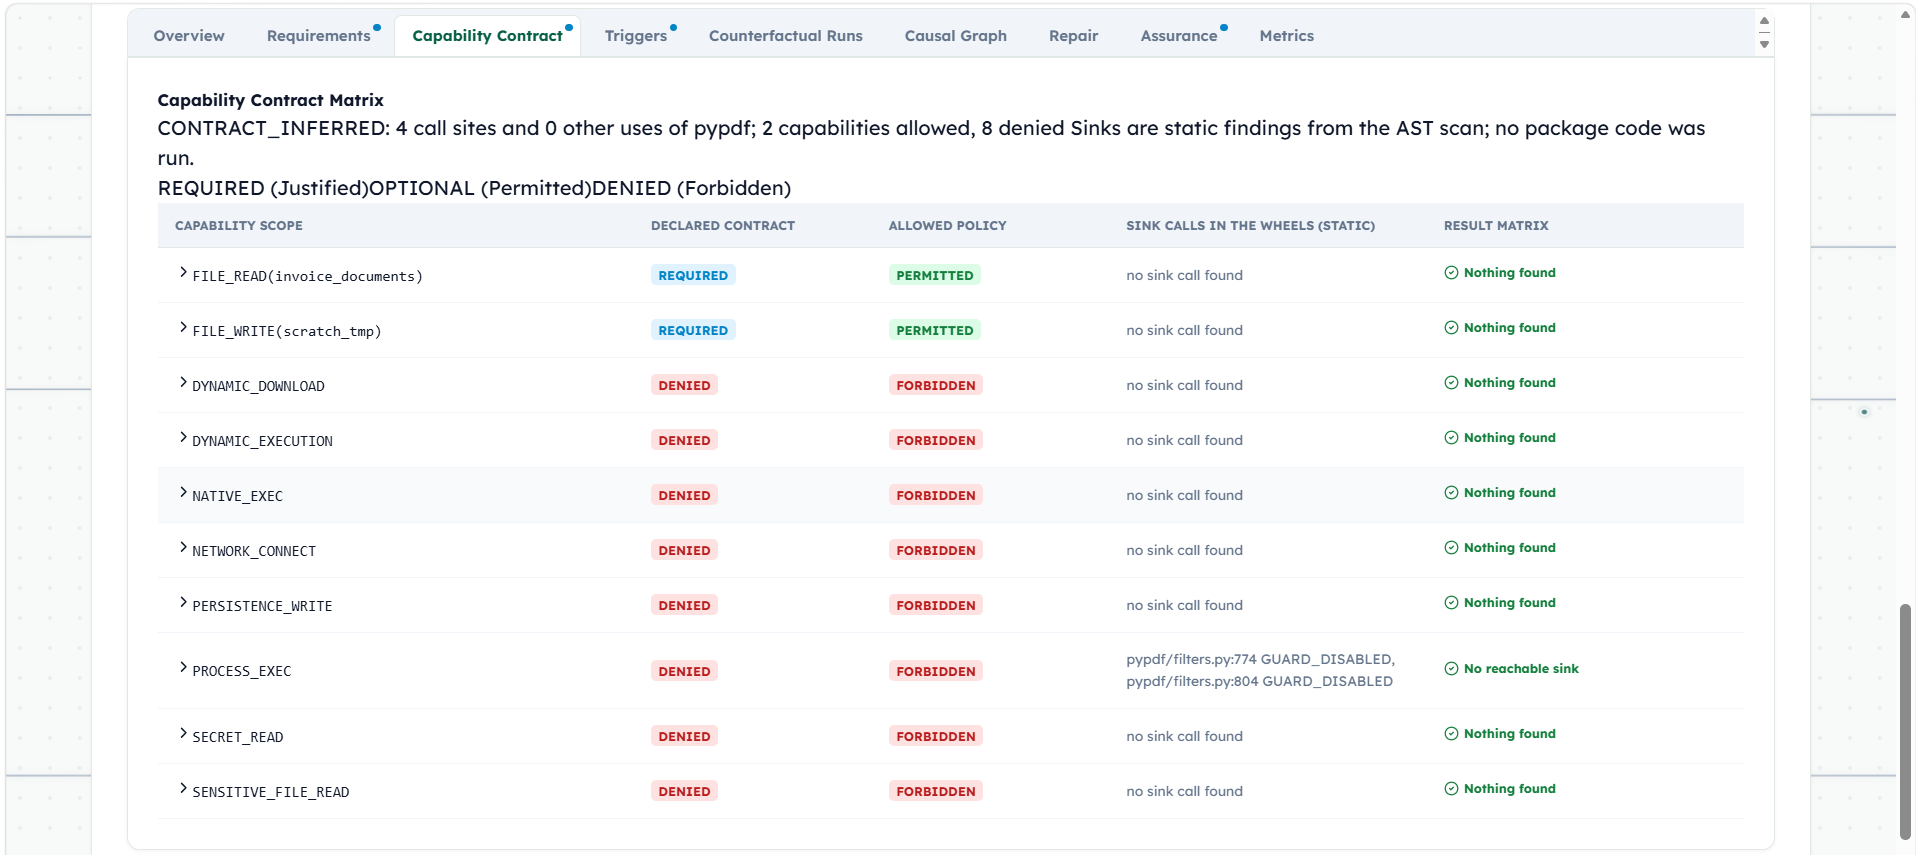
\includegraphics[width=0.9\linewidth]{figures/cavr/cavr-11-capability-contract.png}
    \caption[Capability contract inferred for pypdf 6.19.0]{Capability contract tab for \texttt{pypdf} 6.19.0 in the sample project: two capabilities required and permitted, eight denied, and the two \texttt{subprocess.run} sinks under \texttt{PROCESS\_EXEC} judged \texttt{GUARD\_DISABLED}.}
    \label{fig:cavr-capability-contract}
\end{figure}

\begin{figure}[htbp]
    \centering
    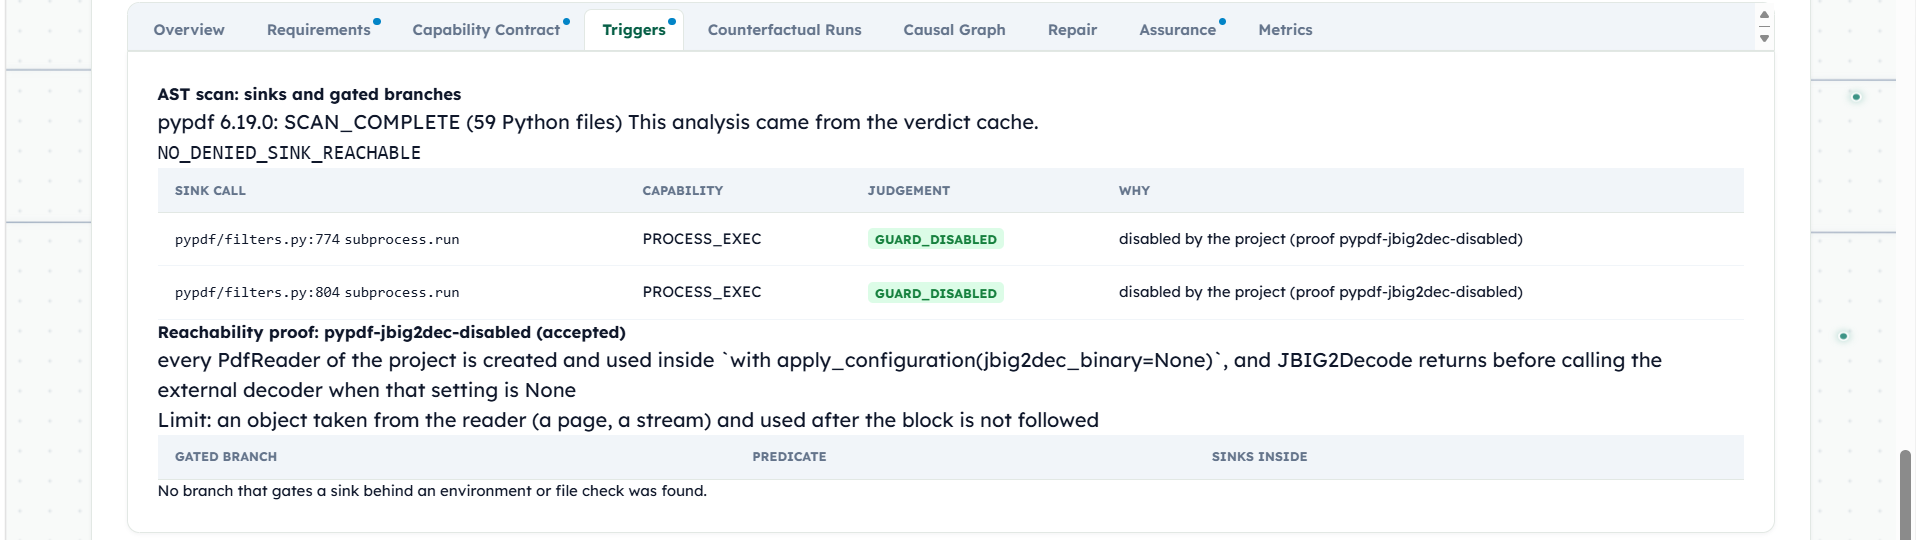
\includegraphics[width=0.9\linewidth]{figures/cavr/cavr-12-ast-scan-sinks.png}
    \caption[AST scan and sink judgement for pypdf 6.19.0]{Triggers tab for \texttt{pypdf} 6.19.0: the AST scan of 59 Python files, the two \texttt{subprocess.run} sinks judged \texttt{GUARD\_DISABLED}, and the accepted reachability proof with its stated limit.}
    \label{fig:cavr-ast-scan}
\end{figure}

\begin{sloppypar}
\textbf{Verdict cache.} \path{cache_key} refuses to build a key unless all eight fields are usable, then hashes their canonical JSON. \path{store} accepts only \texttt{VERIFIED} and \texttt{REJECTED} results. \path{lookup} uses a row only if its integrity digest matches and its own eight columns give the key it is filed under. Only the scan and sink analysis is cached. The download, the tree, the contract and the OSV query run on every request, because the first three are fields of the key and advisories change while the file does not.
\end{sloppypar}

\begin{sloppypar}
\textbf{Pip wrapper.} \path{main} removes the wrapper's own options, calls \path{verify_request} on the remaining pip command, prints the verdict and evidence, and returns the exit code. With \path{--install} and a \texttt{VERIFIED} verdict, \path{install_plan} writes one line \path{name==version} \path{--hash=sha256:<digest>} per node of the verified tree, and pip is run once with a fixed option list: \path{--isolated}, \path{--index-url} \path{https://pypi.org/simple/}, \path{--require-hashes}, \path{--no-deps} and \path{--only-binary} \path{:all:}. The user's own pip arguments are never passed to pip.
\end{sloppypar}

\begin{sloppypar}
\textbf{Dashboard.} \path{run_verification} runs the pipeline in a worker thread and publishes one event per stage that ran, with every value copied from the verdict. \path{stage_summary} builds the six-stage timeline (capture, gate, artifact, cache, analysis, verdict); a stage with no value is marked as not run. Two demo conditions exist and only replace the network transport: \texttt{tampered\_wheel} flips one bit of the downloaded file and \texttt{network\_off} fails every request. A run under a demo condition gets no store, so it is not logged, not cached and not counted in the metrics, and it downloads into its own directory.
\end{sloppypar}

\begin{sloppypar}
Figure~\ref{fig:cavr-timeline-verified} shows the page after chip 1: the six stages of \path{stage_summary} with the value each one returned, and the reasoning panel below them. A tick marks a stage that ran, not a stage that passed; the verdict is the status under the last stage. Figure~\ref{fig:cavr-verdict-verified} shows the verdict card for the same chip. The card prints two words: a header, which is \texttt{ALLOW} for \texttt{VERIFIED}, \texttt{BLOCK} for \texttt{REJECTED} and \texttt{BLOCK}, and \texttt{NEEDS\_REVIEW} for \texttt{UNRESOLVED}, and below it the policy state, which is the CAVR verdict. The screenshots in this report were taken in one browser session on 2026-10-11. The server had already verified pypdf 6.19.0 in that session, so this run shows a cache \texttt{HIT}.
\end{sloppypar}

\begin{figure}[htbp]
    \centering
    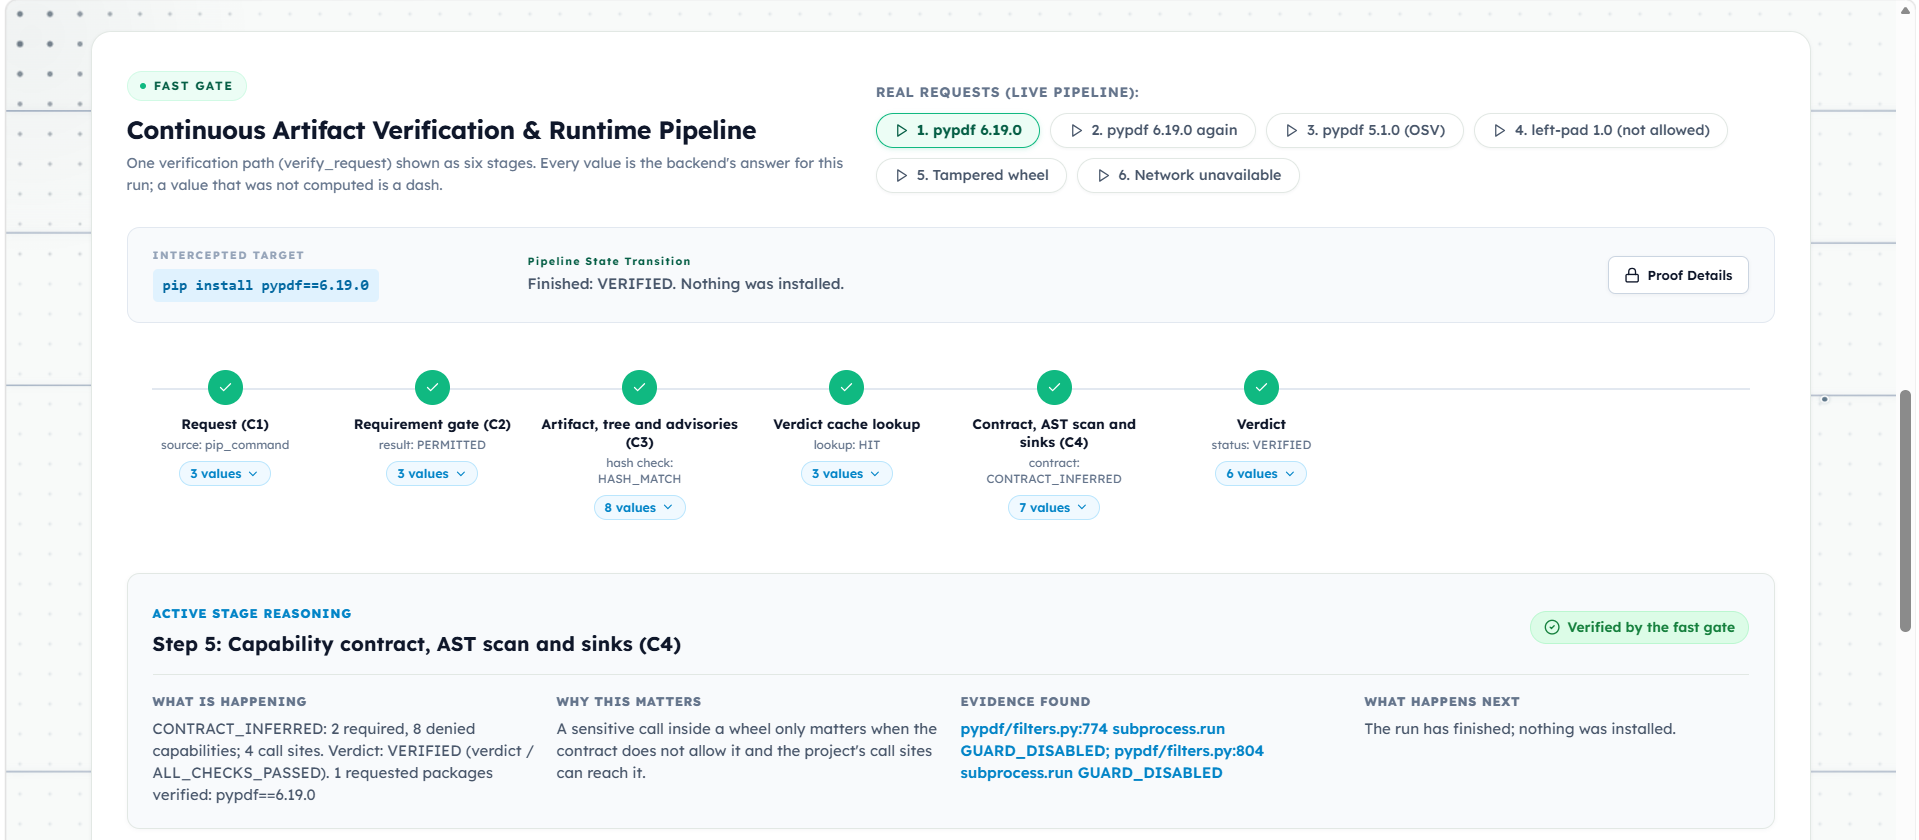
\includegraphics[width=0.9\linewidth]{figures/cavr/cavr-01-verified-pipeline.png}
    \caption[Six-stage timeline for a VERIFIED request]{CAVR page after chip 1, \texttt{pip install pypdf==6.19.0}: all six stages of the timeline ran and the verdict is \texttt{VERIFIED}. The cache lookup is a \texttt{HIT} because the server had verified this wheel earlier in the session. Nothing was installed.}
    \label{fig:cavr-timeline-verified}
\end{figure}

\begin{figure}[htbp]
    \centering
    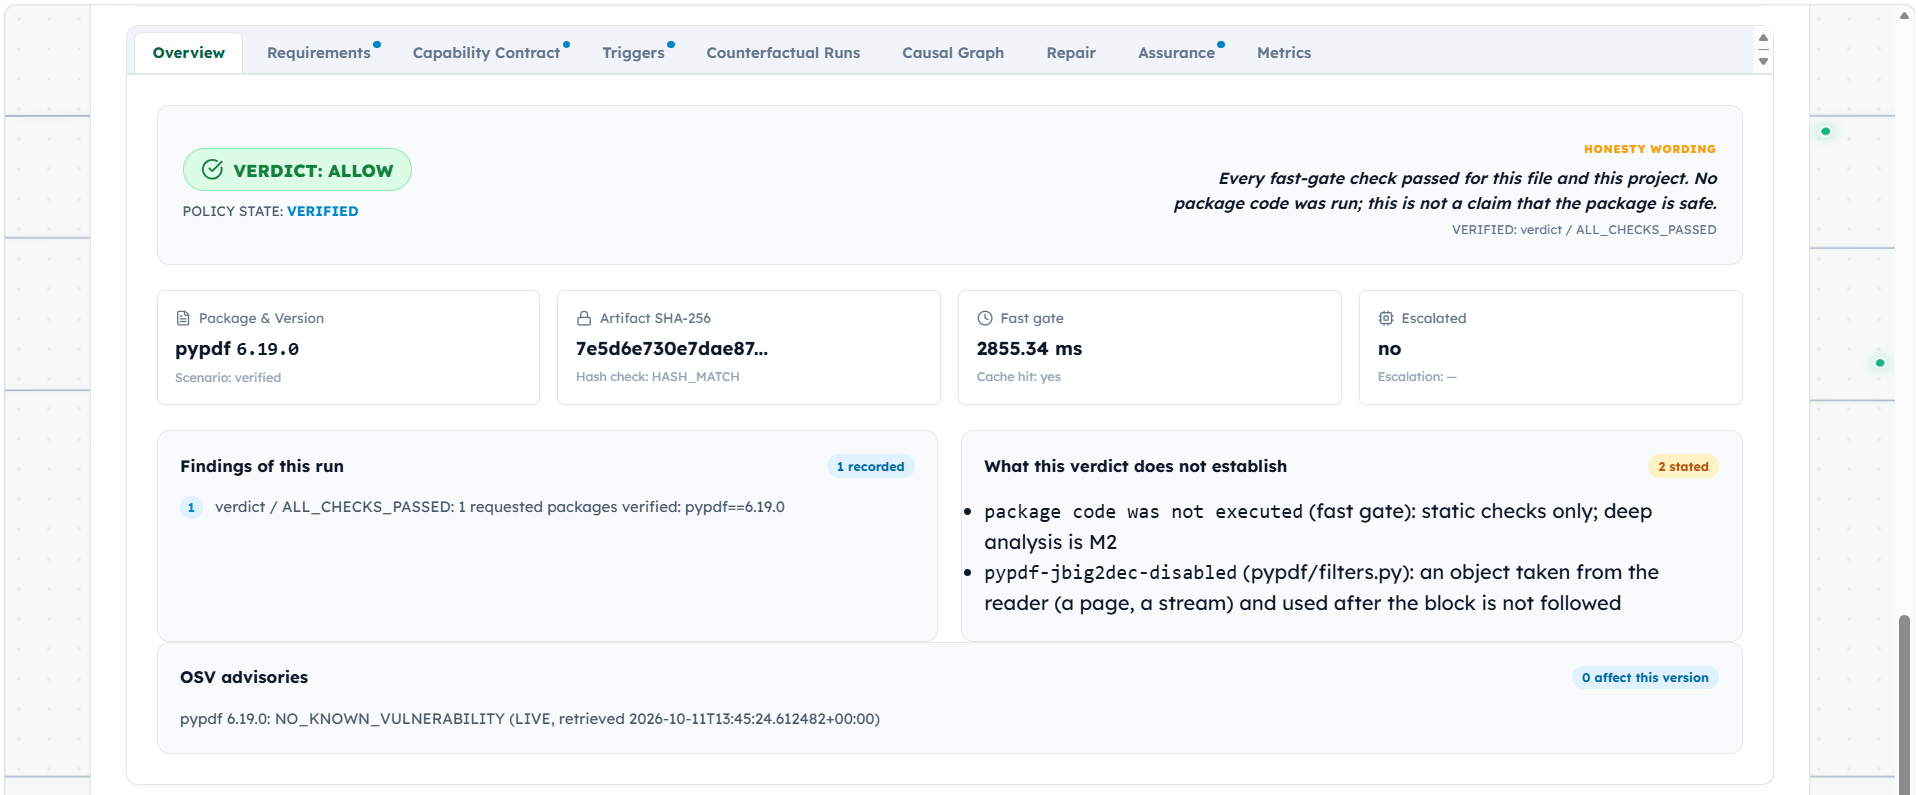
\includegraphics[width=0.9\linewidth]{figures/cavr/cavr-02-verified-verdict.png}
    \caption[Verdict card for a VERIFIED request]{Verdict card for \texttt{pypdf} 6.19.0: policy state \texttt{VERIFIED}, the artifact SHA-256 with \texttt{HASH\_MATCH}, the live OSV answer with no advisory for this version, and the two limits the verdict states.}
    \label{fig:cavr-verdict-verified}
\end{figure}

\begin{sloppypar}
Figure~\ref{fig:cavr-certificate-verified} shows the Assurance tab for another \texttt{VERIFIED} run of the same request in that session. The seven records are the \path{EvidenceChain} of the run, each hashed together with the SHA-256 of the record before it. The certificate below them is built by \path{certificate_for_verdict}: it repeats the verdict and lists the artifact, subtree and contract digests and the result of each check, with sandbox execution as \texttt{NOT\_RUN (M2)}. Figure~\ref{fig:cavr-certificate-limits} shows the limits the page prints below a certificate.
\end{sloppypar}

\begin{figure}[htbp]
    \centering
    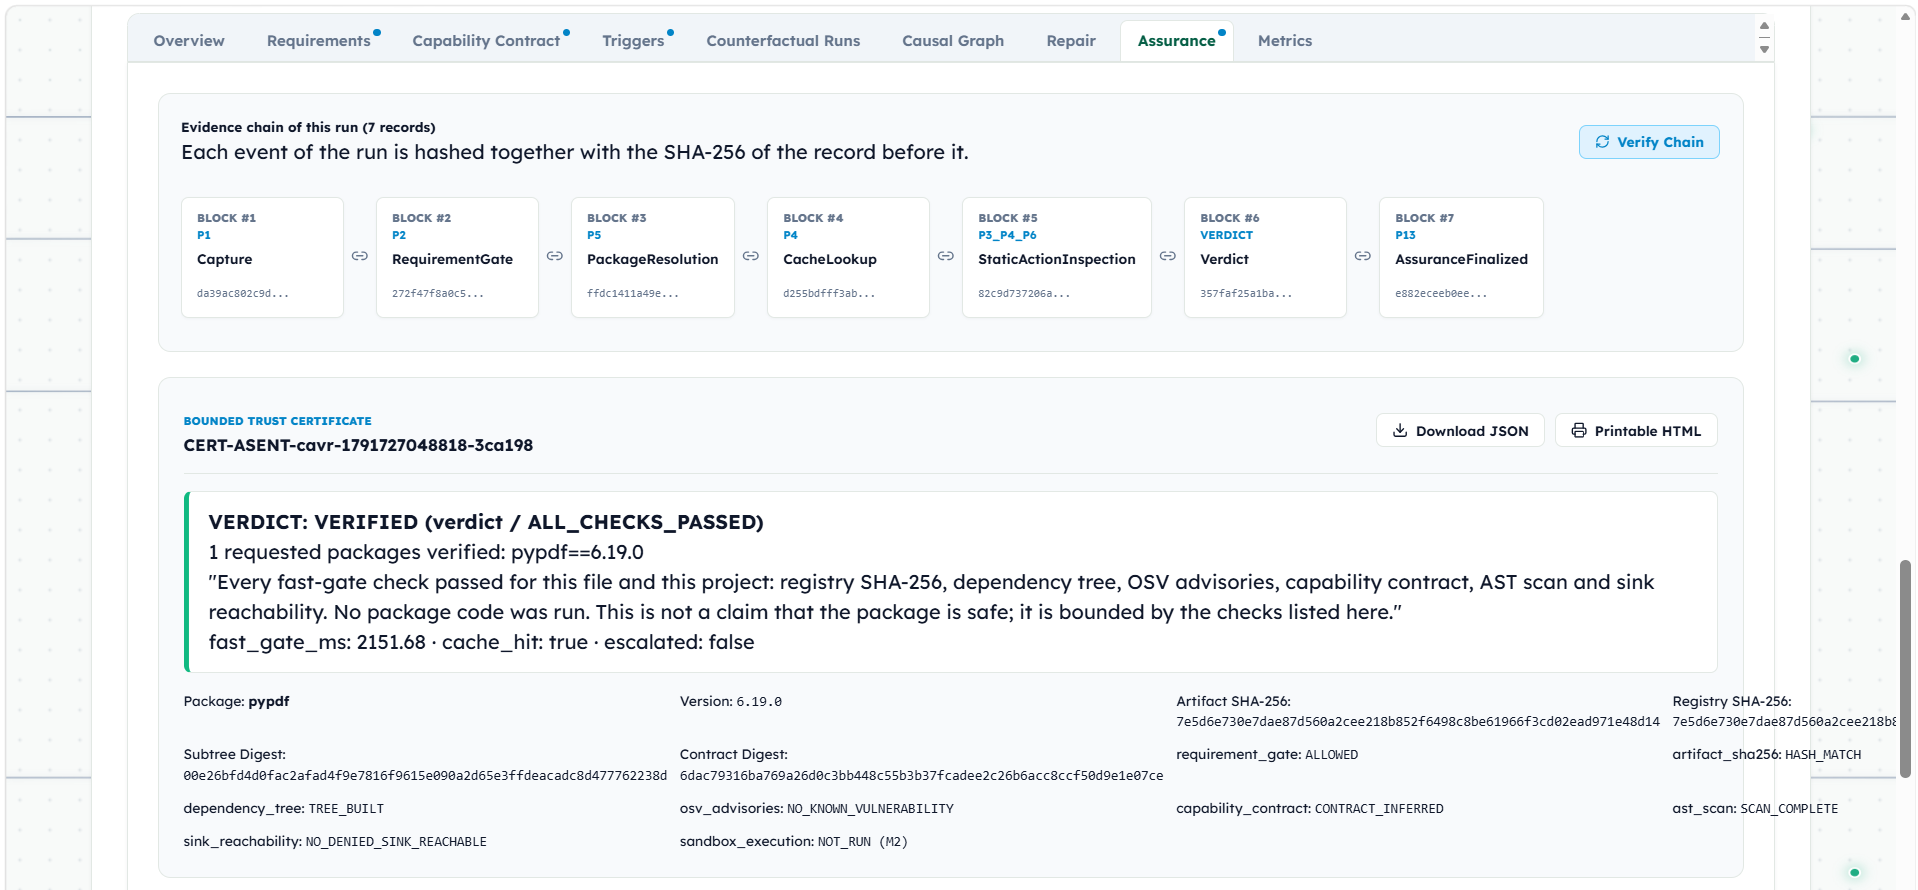
\includegraphics[width=0.9\linewidth]{figures/cavr/cavr-15-assurance-certificate-verified.png}
    \caption[Evidence chain and certificate for a VERIFIED run]{Assurance tab for a \texttt{VERIFIED} run of \texttt{pypdf} 6.19.0: the seven-record evidence chain and the bounded trust certificate with the digests and the result of each check. The right end of the registry digest is cut off by the browser window.}
    \label{fig:cavr-certificate-verified}
\end{figure}

\begin{figure}[htbp]
    \centering
    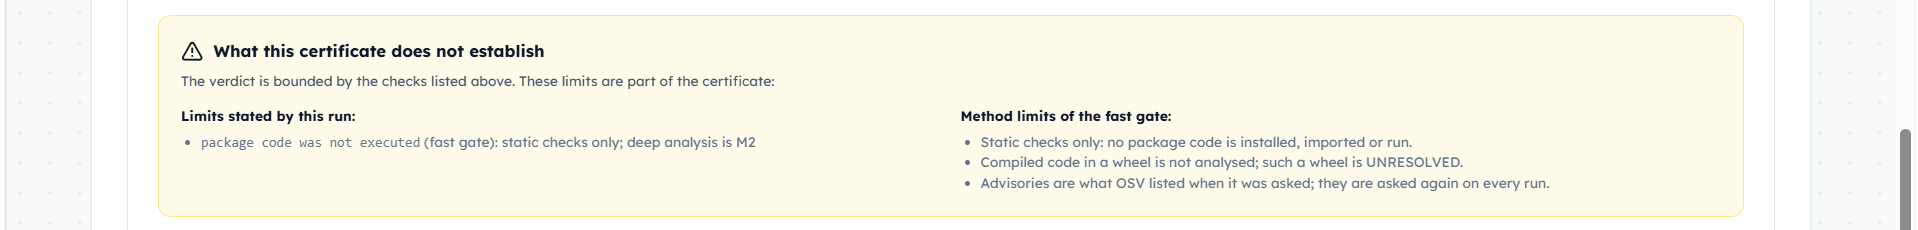
\includegraphics[width=0.9\linewidth]{figures/cavr/cavr-17-certificate-limits.png}
    \caption[Stated limits of a certificate]{``What this certificate does not establish'': the limits stated by the run and the method limits of the fast gate, as printed below a certificate.}
    \label{fig:cavr-certificate-limits}
\end{figure}

\subsection{Algorithms and Technical Decisions}
\setlength{\tabcolsep}{3pt}
\begin{longtable}{p{0.28\textwidth}p{0.25\textwidth}p{0.38\textwidth}}
\toprule
\textbf{Decision} & \textbf{Alternative considered} & \textbf{Why}\\
\midrule
\endhead
Unknown is \texttt{UNRESOLVED} at every stage. & Treat a missing value as zero or as clean. & A missing measurement is not a measurement of zero. A fail-open default would let a network error or an unread file end as \texttt{VERIFIED}.\\
Explicit pip option tables. & Skip every token that starts with a dash, as the old wrapper did. & The old way read the value of \path{-i}, \path{-t} or \path{--index-url} as a package name.\\
An unknown pip option makes the record incomplete. & Guess whether it takes a value, or ignore it. & Guessing either way could hide a package or invent one.\\
Hash the file after it is written, by reading it back. & Hash the chunks while streaming. & The evidence then describes the exact file the later stages open. The cost is reading the file twice.\\
Keep a mismatching file as \path{<filename>.rejected}. & Delete it, or keep the wheel name. & It stays as evidence, and no later stage can open it by its wheel name.\\
Verify the wheel for the running interpreter. & Verify every wheel of the release, or accept only pure-Python wheels. & It is the file pip would install on this machine. Pure-only would make every package with native wheels \texttt{UNRESOLVED}.\\
Check OSV ranges locally as a second reading of OSV's answer. & Trust OSV's answer alone. & If the two readings disagree, one of them is wrong, so the result is \texttt{UNRESOLVED} and not clean.\\
Cache only the scan and sink analysis; never the advisory result. & Cache the final verdict. & A cached \texttt{VERIFIED} must become \texttt{REJECTED} the day OSV lists the version, and a cached rejection must lift if the advisory is withdrawn.\\
Never store \texttt{UNRESOLVED} or \texttt{BLOCK} in the cache. & Cache everything with a short lifetime. & Storing \texttt{UNRESOLVED} would freeze a network failure. \texttt{BLOCK} is decided before any artifact exists, so there is nothing to key on.\\
Reachability is the import closure from the modules the project imports. & A full call graph, or treat every sink as reachable once the package is used. & It needs no execution and still leaves a real unreachable class, such as a command-line module nobody imports.\\
The wrapper passes pip a fixed option list and a generated hash-pinned file. & Append \path{--require-hashes} to the user's command. & An option the capture does not model could otherwise change what pip does.\\
No Docker gives \texttt{UNRESOLVED}; package code never runs on the host. & Keep the host run with the Python audit hook. & The audit hook is not isolation; untrusted code would run with the user's rights.\\
Demo runs get no store. & Log them under a separate label. & An arranged hash mismatch or a 3~ms network-off run is not a measurement, and without a store it cannot touch the cache.\\
Report \texttt{fast\_gate\_ms} per verdict and per cache lookup. & One p50 and p95 over all verdicts. & A \texttt{BLOCK} takes about 2~ms and would pull down the time reported for verifying a package.\\
\bottomrule
\end{longtable}
\setlength{\tabcolsep}{6pt}

\subsection{Tools, Frameworks and Technologies}
\begin{sloppypar}
CAVR is written in Python. The development machine runs Python 3.14.4 and the CI workflow runs Python 3.12. It uses the \texttt{packaging} library for requirement, version and wheel-tag parsing, \texttt{httpx} for HTTPS, and the standard-library modules \texttt{ast}, \texttt{zipfile}, \texttt{hashlib}, \texttt{shlex} and \texttt{sqlite3}. The endpoints are FastAPI routes. The page is React and TypeScript. Tests use pytest, and the page-rendering tests also need Node.js. The two external data sources are the PyPI JSON API with \path{files.pythonhosted.org} and the OSV database, reached through the existing \path{backend/integrations/osv_adapter.py}. GitHub Actions runs the suite with Docker and Podman disabled.
\end{sloppypar}

\begin{sloppypar}
Docker is needed only by the sandbox runner, which the fast gate does not call. Docker is not installed on the development machine, so the real container path has not been executed; every sandbox-runner test replaces the process launcher.
\end{sloppypar}

\begin{sloppypar}
\textbf{Tool use.} I used Claude Code (Anthropic) throughout this iteration. It generated the code changes in \path{backend/cavr/}, the tests in \path{tests/test_cavr_*.py}, the page components and the working notes, following a written plan and the branch rules in \path{CLAUDE.md}. Each batch of plan steps was then read by \texttt{cavr-reviewer}, a read-only Claude Code subagent, and the blocking findings were fixed in a separate commit. My part was to set the scope and the rules, approve the plan steps and the batch workflow, and make the decisions the notes record as mine: for the first step I read the four reviewer reports and decided the outcome of each finding, including which to defer; I chose between the options for the forged-report fix; I wrote the list of six demo issues and the expected verdict of each chip; and I reported the two CI failures and set the rule for fixing the second. For the batches in between, the notes record that the steps ran without a stop and list the open choices left for me. Verification was by pytest, by running new tests against the old code, by fault injection, and by live runs against PyPI and OSV. No project source code is sent to PyPI or OSV; they receive the package name and version only. \textbf{TODO: state which CAVR files I have since read line by line, and which open choices from the notes I have decided.}
\end{sloppypar}

\subsection{Reproducible Setup and Run Instructions}
On Linux, from the repository root:
\begin{sloppypar}
\begin{enumerate}
    \item \texttt{bash} \path{scripts/setup.sh} creates \path{.venv}, installs \path{requirements.lock.txt} and builds the dashboard. It needs Python 3.11 or newer, and npm to build the dashboard.
    \item \texttt{npm} \path{--prefix} \texttt{frontend} \texttt{run} \texttt{build} rebuilds the dashboard after any frontend change. The build output \path{frontend/dist} is not in Git.
    \item \texttt{export} \path{ASENT_DATA=$PWD/runtime-demo} selects an empty data directory, so the first request is a cache miss.
    \item \path{.venv/bin/python} \path{-m} \path{uvicorn} \path{backend.main:app} \path{--host} \path{127.0.0.1} \path{--port} \path{8000} starts the app with the same \texttt{ASENT\_DATA}. Open \path{http://127.0.0.1:8000} and go to the CAVR module.
    \item The pip wrapper is run as \path{.venv/bin/python} \path{-m} \path{backend.cavr.pip_shim} \path{--cavr-project} \path{backend/cavr/sample_project} \path{--cavr-policy} \path{backend/cavr/project_policy.json} \texttt{install} \path{pypdf==6.19.0}.
\end{enumerate}
\end{sloppypar}
The fast gate needs internet access to reach PyPI and OSV. Nothing is installed by any of these commands. The full demo script with the recorded output of every command is \path{docs/cavr-demo.md} on the \texttt{cavr} branch.

\subsection{Demonstration Evidence}\label{sec:cavr-demo}
\begin{sloppypar}
The six cases below are the six chips of the CAVR page. Each was run through \texttt{POST} \path{/api/cavr/run?scenario=<id>}, which is what a chip click calls. The output was recorded on 2026-10-11 at commit \texttt{42e2524} with Python 3.14.4 and Node.js v22.22.1 on WSL2, with internet access. Nothing in these runs uses fixture data. The time column is \texttt{fast\_gate\_ms}, the wall time of the whole request.
\end{sloppypar}

\setlength{\tabcolsep}{3pt}
\begin{longtable}{p{0.04\textwidth}p{0.24\textwidth}p{0.36\textwidth}p{0.11\textwidth}p{0.14\textwidth}}
\toprule
\textbf{No.} & \textbf{Request} & \textbf{Verdict, stage and rule} & \textbf{Cache} & \textbf{Time (ms)}\\
\midrule
\endhead
1 & \texttt{pip install pypdf==6.19.0} & \texttt{VERIFIED}, \texttt{verdict}, \texttt{ALL\_CHECKS\_PASSED}; \texttt{HASH\_MATCH} & \texttt{MISS} & 3912.65\\
2 & The same request again & \texttt{VERIFIED}, \texttt{verdict}, \texttt{ALL\_CHECKS\_PASSED}; \texttt{HASH\_MATCH} & \texttt{HIT} & 2117.81\\
3 & \texttt{pip install pypdf==5.1.0} & \texttt{REJECTED}, \texttt{advisories}, \texttt{KNOWN\_VULNERABILITY}; \texttt{HASH\_MATCH}; 97 advisories & \texttt{MISS} & 2919.3\\
4 & \texttt{pip install left-pad==1.0} & \texttt{BLOCK}, \texttt{gate}, \texttt{NOT\_ON\_ALLOWLIST}; nothing downloaded & not reached & 2.17\\
5 & \texttt{pip install pypdf==6.19.0}, one bit of the wheel flipped on the way in & \texttt{REJECTED}, \texttt{artifact}, \texttt{HASH\_MISMATCH} & not reached & 1582.34\\
6 & \texttt{pip install pypdf==6.19.0}, PyPI unreachable & \texttt{UNRESOLVED}, \texttt{artifact}, \texttt{REGISTRY\_UNAVAILABLE} & not reached & 3.09\\
\bottomrule
\end{longtable}
\setlength{\tabcolsep}{6pt}

\begin{sloppypar}
In cases 1 and 2 the SHA-256 computed from the downloaded file and the registry digest are both \path{7e5d6e730e7dae87d560a2cee218b852f6498c8be61966f3cd02ead971e48d14}. In case 5 the registry digest is the same value and the file that arrived hashes to \path{a52a19f9f614cd13e3f7544c78e5a44fc0996507c8b1b620abd45da5d73ee7b9}. The rejected file is kept under \path{quarantine-demo/tampered_wheel/}, and the genuine wheel in \path{quarantine/} had the same SHA-256 before and after the tampered run. In case 3 the reason names the count and the first three OSV identifiers (\texttt{GHSA-23w6-3w8w-8484}, \texttt{GHSA-248m-82v9-q6g6}, \texttt{GHSA-2q4j-m29v-hq73}) ``and 94 more''; the count grows when OSV publishes more. In case 4 the quarantine directory holds only the two pypdf wheels of cases 1 to 3. In case 6 the same request that was verified and cached in cases 1 and 2 is not served from the cache, because the SHA-256 of the downloaded file is one of the eight key fields.
\end{sloppypar}

\begin{sloppypar}
The blocks below are the recorded output of those runs, copied from \path{docs/cavr-demo.md}. Each was printed by the two helper functions of the demo script, which call \texttt{POST} \path{/api/cavr/run?scenario=<id>} and then read \texttt{GET} \path{/api/cavr/proof/{run_id}}. Lines longer than the page are wrapped here with an indent; nothing else is changed. The run id and \texttt{fast\_gate\_ms} differ on every run.
\end{sloppypar}

\noindent Case 1, chip ``1. pypdf 6.19.0'': verified, cache miss.
\begin{singlespace}
\scriptsize
\begin{verbatim}
run id: cavr-1791668207427-c7286f
request: pip install pypdf==6.19.0
verdict: VERIFIED | stage: verdict | rule: ALL_CHECKS_PASSED
reason: 1 requested packages verified: pypdf==6.19.0
demo condition: None
hash expected (registry): 7e5d6e730e7dae87d560a2cee218b852f6498c8be61966f3cd02ead971e48d14
hash of what arrived:     7e5d6e730e7dae87d560a2cee218b852f6498c8be61966f3cd02ead971e48d14
hash result: HASH_MATCH | matches: True
fast_gate_ms: 3912.65 | cache_hit: False | escalated: False | logged: True
  stage capture  ran         | source: pip_command
  stage gate     ran         | result: PERMITTED
  stage artifact ran         | hash check: HASH_MATCH
  stage cache    ran         | lookup: MISS
  stage analysis ran         | contract: CONTRACT_INFERRED
  stage verdict  ran         | status: VERIFIED
\end{verbatim}
\end{singlespace}

\noindent Case 3, chip ``3. pypdf 5.1.0 (OSV)'': the genuine wheel, rejected by the advisory check.
\begin{singlespace}
\scriptsize
\begin{verbatim}
run id: cavr-1791668213619-9f0f52
request: pip install pypdf==5.1.0
verdict: REJECTED | stage: advisories | rule: KNOWN_VULNERABILITY
reason: pypdf==5.1.0: pypdf 5.1.0 is affected by 97 known advisories: GHSA-23w6-3w8w-8484,
      GHSA-248m-82v9-q6g6, GHSA-2q4j-m29v-hq73 and 94 more
demo condition: None
hash expected (registry): 3bd4f503f4ebc58bae40d81e81a9176c400cbbac2ba2d877367595fb524dfdfc
hash of what arrived:     3bd4f503f4ebc58bae40d81e81a9176c400cbbac2ba2d877367595fb524dfdfc
hash result: HASH_MATCH | matches: True
fast_gate_ms: 2919.3 | cache_hit: False | escalated: False | logged: True
  stage capture  ran         | source: pip_command
  stage gate     ran         | result: PERMITTED
  stage artifact ran         | hash check: HASH_MATCH
  stage cache    ran         | lookup: MISS
  stage analysis ran         | contract: CONTRACT_INFERRED
  stage verdict  ran         | status: REJECTED
\end{verbatim}
\end{singlespace}

\noindent Case 4, chip ``4. left-pad 1.0 (not allowed)'': blocked at the gate. The last two lines are the listing of the quarantine directory, which holds only the wheels of cases 1 to 3.
\begin{singlespace}
\scriptsize
\begin{verbatim}
run id: cavr-1791668216623-a934f6
request: pip install left-pad==1.0
verdict: BLOCK | stage: gate | rule: NOT_ON_ALLOWLIST
reason: left-pad is not on the project allowlist
demo condition: None
hash expected (registry): None
hash of what arrived:     None
hash result: None | matches: None
fast_gate_ms: 2.17 | cache_hit: False | escalated: False | logged: True
  stage capture  ran         | source: pip_command
  stage gate     ran         | result: BLOCK
  stage artifact did not run | hash check: None
  stage cache    did not run | lookup: None
  stage analysis did not run | contract: None
  stage verdict  ran         | status: BLOCK
pypdf-5.1.0-py3-none-any.whl
pypdf-6.19.0-py3-none-any.whl
\end{verbatim}
\end{singlespace}

\noindent Case 5, chip ``5. Tampered wheel'': the first line is \texttt{sha256sum} of the genuine wheel before the run; the last four lines are the quarantine listing and \texttt{sha256sum} of the genuine wheel and of the rejected file after it.
\begin{singlespace}
\scriptsize
\begin{verbatim}
7e5d6e730e7dae87d560a2cee218b852f6498c8be61966f3cd02ead971e48d14
      runtime-demo/cavr/quarantine/pypdf-6.19.0-py3-none-any.whl
run id: cavr-1791668228892-f6e43c
request: pip install pypdf==6.19.0
verdict: REJECTED | stage: artifact | rule: HASH_MISMATCH
reason: pypdf==6.19.0: pypdf-6.19.0-py3-none-any.whl: SHA-256 of the downloaded file is
      a52a19f9f614cd13e3f7544c78e5a44fc0996507c8b1b620abd45da5d73ee7b9, the registry says
      7e5d6e730e7dae87d560a2cee218b852f6498c8be61966f3cd02ead971e48d14
demo condition: tampered_wheel
hash expected (registry): 7e5d6e730e7dae87d560a2cee218b852f6498c8be61966f3cd02ead971e48d14
hash of what arrived:     a52a19f9f614cd13e3f7544c78e5a44fc0996507c8b1b620abd45da5d73ee7b9
hash result: HASH_MISMATCH | matches: False
fast_gate_ms: 1582.34 | cache_hit: False | escalated: False | logged: False
  stage capture  ran         | source: pip_command
  stage gate     ran         | result: PERMITTED
  stage artifact ran         | hash check: HASH_MISMATCH
  stage cache    did not run | lookup: None
  stage analysis did not run | contract: None
  stage verdict  ran         | status: REJECTED
pypdf-5.1.0-py3-none-any.whl
pypdf-6.19.0-py3-none-any.whl
7e5d6e730e7dae87d560a2cee218b852f6498c8be61966f3cd02ead971e48d14
      runtime-demo/cavr/quarantine/pypdf-6.19.0-py3-none-any.whl
a52a19f9f614cd13e3f7544c78e5a44fc0996507c8b1b620abd45da5d73ee7b9
      runtime-demo/cavr/quarantine-demo/tampered_wheel/pypdf-6.19.0-py3-none-any.whl.rejected
\end{verbatim}
\end{singlespace}

\noindent Case 6, chip ``6. Network unavailable'': unresolved, although the same request was verified and cached in cases 1 and 2.
\begin{singlespace}
\scriptsize
\begin{verbatim}
run id: cavr-1791668230579-72878e
request: pip install pypdf==6.19.0
verdict: UNRESOLVED | stage: artifact | rule: REGISTRY_UNAVAILABLE
reason: pypdf==6.19.0: cannot read the registry: ConnectError: the network is off (dashboard demo
      condition)
demo condition: network_off
hash expected (registry): None
hash of what arrived:     None
hash result: REGISTRY_UNAVAILABLE | matches: None
fast_gate_ms: 3.09 | cache_hit: False | escalated: False | logged: False
  stage capture  ran         | source: pip_command
  stage gate     ran         | result: PERMITTED
  stage artifact ran         | hash check: REGISTRY_UNAVAILABLE
  stage cache    did not run | lookup: None
  stage analysis did not run | contract: None
  stage verdict  ran         | status: UNRESOLVED
\end{verbatim}
\end{singlespace}

The same requests were run through the pip wrapper in the same data directory:

\setlength{\tabcolsep}{3pt}
\begin{longtable}{p{0.40\textwidth}p{0.38\textwidth}p{0.12\textwidth}}
\toprule
\textbf{Wrapper request} & \textbf{Verdict, stage and rule} & \textbf{Exit code}\\
\midrule
\endhead
\texttt{install pypdf==6.19.0} & \texttt{VERIFIED}, \texttt{verdict}, \texttt{ALL\_CHECKS\_PASSED}; cache \texttt{HIT} & 0\\
\texttt{install pypdf==5.1.0} & \texttt{REJECTED}, \texttt{advisories}, \texttt{KNOWN\_VULNERABILITY} & 1\\
\texttt{install left-pad==1.0} & \texttt{BLOCK}, \texttt{gate}, \texttt{NOT\_ON\_ALLOWLIST} & 3\\
\texttt{install pypdf==6.19.0} with every HTTPS request sent to a local port where nothing listens & \texttt{UNRESOLVED}, \texttt{artifact}, \texttt{REGISTRY\_UNAVAILABLE} (``Connection refused'') & 2\\
\bottomrule
\end{longtable}
\setlength{\tabcolsep}{6pt}

\noindent Wrapper run for \texttt{pypdf==6.19.0}, with the evidence of every stage and exit code 0. It was run after cases 1 to 6 in the same data directory, so it is a cache hit on the analysis the dashboard stored.
\begin{singlespace}
\scriptsize
\begin{verbatim}
CAVR verdict: VERIFIED
  stage: verdict   rule: ALL_CHECKS_PASSED
  reason: 1 requested packages verified: pypdf==6.19.0
  request: pip install pypdf==6.19.0
  fast_gate_ms: 2161.04   cache_hit: True   escalated: False
  gate: PERMITTED (ALLOWED)   policy version:
      e4b357a45bb7400290f240991bbe174606fafa750e9fd08dba7fb18c0984fc46
package pypdf==6.19.0: VERIFIED (verdict / ALL_CHECKS_PASSED)
  reason: hash, tree, advisories and contract checked; 2 sink calls found; none is both denied by
      the contract and reachable from the project
  artifact: pypdf-6.19.0-py3-none-any.whl HASH_MATCH
    sha256 7e5d6e730e7dae87d560a2cee218b852f6498c8be61966f3cd02ead971e48d14
    registry 7e5d6e730e7dae87d560a2cee218b852f6498c8be61966f3cd02ead971e48d14
  tree: TREE_BUILT, 1 file(s), subtree digest
      00e26bfd4d0fac2afad4f9e7816f9615e090a2d65e3ffdeacadc8d477762238d
    pypdf==6.19.0 sha256 7e5d6e730e7dae87d560a2cee218b852f6498c8be61966f3cd02ead971e48d14
  contract: CONTRACT_INFERRED, 4 call site(s), digest
      6dac79316ba769a26d0c3bb448c55b3b37fcadee2c26b6acc8ccf50d9e1e07ce
  advisories: pypdf 6.19.0 NO_KNOWN_VULNERABILITY
  scan: pypdf SCAN_COMPLETE (59 Python files)
  sink: pypdf/filters.py:774 subprocess.run GUARD_DISABLED
  sink: pypdf/filters.py:804 subprocess.run GUARD_DISABLED
  cache: HIT
install: not requested; nothing was installed (run again with --install after a VERIFIED verdict)
exit code: 0
\end{verbatim}
\end{singlespace}

\begin{sloppypar}
The last wrapper run is a real connection failure with no demo switch. For the verified request the wrapper also printed the evidence of each stage: the tree has one node, the contract has four call sites, the scan read 59 Python files, and the two \texttt{subprocess.run} sinks in \path{pypdf/filters.py} were both judged \texttt{GUARD\_DISABLED}.
\end{sloppypar}

\begin{sloppypar}
\textbf{Metrics.} After cases 1 to 6 and one more click of chip 2, \texttt{GET} \path{/api/cavr/metrics} reported five logged verdicts: three \texttt{VERIFIED}, one \texttt{REJECTED} and one \texttt{BLOCK}. Cases 5 and 6 are demo-condition runs and are not logged. Two of the five verdicts were cache hits (0.4), which is two of the four verdicts that reached the cache lookup (0.5). The three \texttt{VERIFIED} requests took 3912.65~ms (miss), 2117.81~ms (hit) and 4524.49~ms (hit). A cache hit skips only the AST scan and the sink judgement; the wheel is still downloaded and OSV is still asked, so most of the time is network and one hit was slower than the miss. With one to three requests per group these are observations, not statistics, and I do not claim a speed-up from the cache.
\end{sloppypar}

\begin{sloppypar}
\textbf{Repository.} The \texttt{cavr} branch has 42 commits that are not on \texttt{origin/master}, dated 2026-10-09 to 2026-10-11, all under my name: 13 \texttt{feat(cavr)}, 12 \texttt{fix(cavr)}, one \texttt{refactor(cavr)}, one \texttt{test(cavr)}, 9 \texttt{docs(cavr)}, 4 \texttt{chore(cavr)} and two outside the module. Each plan step is one commit, and each review round has its own fix commit. The commits that carry the features of this chapter are:
\end{sloppypar}

\setlength{\tabcolsep}{3pt}
\begin{longtable}{p{0.13\textwidth}p{0.78\textwidth}}
\toprule
\textbf{Commit} & \textbf{What it contains}\\
\midrule
\endhead
\texttt{3be14db} & Refuse host execution of unpinned package source (sandbox runner).\\
\texttt{73f7892} & C1: parse \texttt{pip install} commands into capture records.\\
\texttt{4c053b6} & C1: capture \path{requirements.txt} edits.\\
\texttt{c018f30} & C2: fail-closed requirement gate.\\
\texttt{31dd229} & Review fix: close two fail-open paths in the gate.\\
\texttt{00b9332} & C3: fetch PyPI release metadata and verify the artifact SHA-256.\\
\texttt{3ba4970} & C3: read wheel metadata safely.\\
\texttt{3cb1a35} & C3: transitive tree and subtree digest.\\
\texttt{b7c98cf} & C3: OSV check with real version ranges.\\
\texttt{c72b56a} & C3: light AST risk scan of wheel sources.\\
\texttt{c9b8852} & Review fix: read \texttt{.pth} files the way \path{site.py} does.\\
\texttt{a188cb6} & C4: capability contract from real imports and call sites.\\
\texttt{d8e6367} & Eight-field verdict cache.\\
\texttt{c5c0ef4} & Single \path{verify_request} pipeline.\\
\texttt{002a69c} & Review fix: close fail-open paths in the sink judgement and the pypdf proof.\\
\texttt{1e17034} & Pip wrapper runs the pipeline before pip.\\
\texttt{ca5a0e2} & Dashboard API uses the pipeline.\\
\texttt{fe9fd4f} & Review fix: keep demo runs out of the report numbers; drop the old trusted-package endpoints.\\
\texttt{384ec4f} & Dashboard chips are six real requests from the scenario API.\\
\texttt{42e2524} & Tampered-wheel demo run works on its own copy. The demo outputs above were recorded at this commit.\\
\texttt{8cafa8a} & Review fix: no ``nothing found'' without a scan, no advisory count without an OSV answer.\\
\texttt{fd276d7} & Find pypdf call sites reached through a vendored local artifact.\\
\texttt{d63183d} & Fix the two defects found by CI. Head of the branch.\\
\bottomrule
\end{longtable}
\setlength{\tabcolsep}{6pt}

\begin{sloppypar}
\textbf{CI.} The workflow \path{.github/workflows/ci.yml} was added in commit \texttt{1d0fe31}. It has six jobs on Python 3.12: lint (byte-compile and a Bandit scan), the CAVR tests (\path{tests/test_cavr_*.py}), the SABLE isolation test, the shared and threat-repository tests, the full suite, and the frontend build. Commits \texttt{1b55cca} and \texttt{4b32eb5} make the test jobs stop Docker and move the \texttt{docker} and \texttt{podman} binaries away before pytest starts, so the sandbox tests run in the no-container mode; a job with a real Docker sandbox is deferred. The runs on the \texttt{cavr} branch are:
\end{sloppypar}

\setlength{\tabcolsep}{3pt}
\begin{longtable}{p{0.16\textwidth}p{0.12\textwidth}p{0.62\textwidth}}
\toprule
\textbf{Run} & \textbf{Commit} & \textbf{Result}\\
\midrule
\endhead
\href{https://github.com/SheharyarAli-Dev/Working-POC/actions/runs/38092518268}{38092518268} & \texttt{7c2bd6b} & Failed in the CAVR tests job and the full-suite job. \textbf{TODO: record which tests failed; the log was not available when this chapter was written.}\\
\href{https://github.com/SheharyarAli-Dev/Working-POC/actions/runs/38135800645}{38135800645} & \texttt{fd276d7} & Failed. CAVR tests job: 1 failed, 1238 passed, 26 skipped. Full-suite job: 2 failed, 1302 passed, 26 skipped. The other four jobs passed.\\
\href{https://github.com/SheharyarAli-Dev/Working-POC/actions/runs/38137109059}{38137109059} & \texttt{d63183d} & All six jobs passed. CAVR tests job: 1254 passed, 26 skipped. Full-suite job: 1319 passed, 26 skipped.\\
\bottomrule
\end{longtable}
\setlength{\tabcolsep}{6pt}

\begin{sloppypar}
The 26 skips in CI are the seven live tests, which need \texttt{CAVR\_LIVE=1}, and the 19 page-rendering tests, which need the frontend's Node modules in the test job. The two failures of run 38135800645 are described in the next subsection.
\end{sloppypar}

\begin{sloppypar}
\textbf{Screenshots.} The recorded output above was produced through the API, without a browser. The page was opened in a browser afterwards, on 2026-10-11, and the six chips were clicked. Case 1 in that session is shown in Figures~\ref{fig:cavr-timeline-verified} and~\ref{fig:cavr-verdict-verified}, and cases 3 to 6 are shown in Section~\ref{sec:cavr-edge}. These are separate runs from the ones recorded above, so the run ids and \texttt{fast\_gate\_ms} differ, and case 1 appears there as a cache \texttt{HIT}.
\end{sloppypar}

\subsection{Defects Found by CI}\label{sec:cavr-ci-defects}
\begin{sloppypar}
Run 38135800645 failed two tests that pass on the development machine. The development machine runs Python 3.14.4 and has no strace, Docker or Podman. CI runs Python 3.12 with Docker and Podman disabled. I reproduced both failures locally with Python 3.12.15 in a virtual environment built from \path{requirements.lock.txt} and a strace 6.19 binary on the path, and fixed both in commit \texttt{d63183d}.
\end{sloppypar}

\begin{sloppypar}
\textbf{Defect 1: \texttt{PermissionError} on Python 3.12.} The failing test was \path{test_directory_that_cannot_be_listed_makes_the_context_unresolved} in \path{tests/test_cavr_contract.py}. It gives the context extractor a project that contains a directory of mode 0 and expects \texttt{UNRESOLVED} with rule \texttt{SOURCE\_NOT\_READ}. In CI it ended with \texttt{PermissionError: [Errno 13] Permission denied}. The cause was in \path{_python_files} in \path{backend/cavr/context_extractor.py}: to skip virtual environments it asked whether \path{pyvenv.cfg} is a file inside each directory, using \path{Path.is_file()}. On a directory that may not be searched, \path{Path.is_file()} raises \texttt{PermissionError} on Python 3.12 and returns false on Python 3.14. So on 3.12 the walk crashed, and on 3.14 the unreadable directory was quietly treated as ``not a virtual environment''. Neither is the fail-closed behaviour the module requires.
\end{sloppypar}

\begin{sloppypar}
The fix replaces the \texttt{pathlib} calls with two helpers, \path{_is_symlink} and \path{_is_virtualenv}, that call \path{os.lstat} and \path{os.stat} directly. ``Not found'' is false; any other \texttt{OSError} is raised to the caller. \path{_python_files} catches it, adds the directory to \texttt{not\_read} and does not enter it, and any \texttt{not\_read} entry makes the context \texttt{UNRESOLVED} \texttt{SOURCE\_NOT\_READ}. The same change fixed two things the old code got wrong on Python 3.14: a directory of mode 444 was not reported as one unreadable directory, and a project directory under a closed parent was called missing. I chose \path{os.stat} over wrapping the \texttt{pathlib} call in \texttt{try} because \texttt{pathlib} hides the error on 3.14, so only the direct call behaves the same on both versions. Four test functions with six cases were added to \path{tests/test_cavr_contract.py}, including \path{test_virtualenv_check_that_fails_makes_the_directory_not_read_on_every_python}, which produces the 3.12 behaviour on any Python by making \path{os.stat} refuse.
\end{sloppypar}

\begin{sloppypar}
\textbf{Defect 2: the no-container mode lost a network event.} The failing test was \path{test_controlled_dormant_execution} in \path{tests/test_modules.py}, with \texttt{assert False} on \texttt{causal\_confirmed}. The test runs the inert lab fixture twice, as a normal run and as the activated counterfactual run, and expects the canary marker to reach the local listener only in the activated run. Without a container the lab runner, \path{run_counterfactual} in \path{backend/cavr/sandbox.py}, uses strace as its monitor when strace is available (execution mode \texttt{PINNED\_INERT\_LAB\_STRACE}) and Python audit events otherwise (\texttt{PINNED\_INERT\_LAB\_PYTHON\_AUDIT}). The development machine has no strace, so it had only ever run the audit mode. The CI log does not print the execution mode; that the runner used strace is concluded from the local reproduction, where the test fails with strace on the path and passes without it, on Python 3.12 and 3.14 alike.
\end{sloppypar}

\begin{sloppypar}
The cause was in \path{normalize} in \path{backend/cavr/runtime_monitor.py}, which turns strace lines into events. It skipped every line whose result is \texttt{-1}. The lab file connects with \path{socket.create_connection} and a timeout, which is a non-blocking connect, and strace prints a non-blocking connect that has started as a \texttt{-1} result (the line is wrapped here):
\end{sloppypar}
\begin{singlespace}
\scriptsize
\begin{verbatim}
connect(4, {sa_family=AF_INET, sin_port=htons(18765), sin_addr=inet_addr("127.0.0.1")}, 16)
      = -1 EINPROGRESS
\end{verbatim}
\end{singlespace}
\begin{sloppypar}
\noindent That line was dropped, so the strace run had no \texttt{NETWORK\_CONNECT} event, no \texttt{NETWORK\_CONNECT} violation and no confirmed secret-read-then-connect correlation. The verdict was still \texttt{REJECTED} and the canary was still received in both modes; what was missing was one event and the evidence built on it. The fix keeps a \texttt{connect} line with \texttt{-1 EINPROGRESS}, because that result means the connection has started and not that it failed. Every other failed system call is still skipped: a refused connect made no connection, and counting attempts belongs to the later sandbox work. I did not weaken the test. Two assertions were added to it (a \texttt{NETWORK\_CONNECT} event in the activated run and none in the normal run), the execution mode is now printed in its assertion messages, and \path{tests/test_cavr_runtime_monitor.py} was added with five test functions and nine cases on eight recorded lines of the real trace. \path{test_the_connection_alone_is_not_a_confirmed_flow} checks that a connect without the received marker, with another payload, without the read, or before the read is not a confirmed flow.
\end{sloppypar}

\begin{sloppypar}
\textbf{After the fix.} The old code failed 9 of the new tests on Python 3.14 without strace and 13 on Python 3.12 with strace, the two CI failures among them. With the fix the full suite reported 1338 passed, 0 failed and 7 skipped on Python 3.14.4 without strace and the same on Python 3.12.15 with strace, and CI run 38137109059 on \texttt{d63183d} passed all six jobs. Three limits remain: a refused or blocked connect and a failed open of a secret file still leave no event; an \texttt{EINPROGRESS} connect is recorded without checking that it completed; and the Docker and Podman modes have not been run anywhere, because neither is installed on the development machine and CI disables both.
\end{sloppypar}

\subsection{Known Limitations}
\begin{itemize}
    \item The fast gate handles PyPI wheels only. A release with no wheel, and VCS, URL and local-path requirements, end \texttt{UNRESOLVED}. npm is not handled.
    \item No package is executed. Behaviour that only appears at run time, and native code, are outside the fast gate; a wheel with a native extension is \texttt{UNRESOLVED}.
    \item The shared orchestrator still calls the older analyzer in \path{backend/cavr/analyzer.py}, which does not go through \path{verify_request}. Moving it was stopped for a decision: the older analyzer accepts PyPI's advisory list when no OSV answer is stored, the pipeline does not, and the change would turn the orchestrator's safe scenario into \texttt{UNRESOLVED} offline.
    \item The advisory record the older analyzer relies on was retrieved on 2026-09-25 and is accepted for 30 days. From 2026-10-25 the integration tests that need pypdf \texttt{VERIFIED} on that path will fail unless a fresh advisory answer is stored.
    \item The \texttt{GUARD\_DISABLED} proof is written for pypdf only. Reachability is an import closure, not a call graph, and cannot see imports built at run time other than \path{__import__} and \path{importlib.import_module}.
    \item Every run downloads the tree again; the cache saves the scan, not the network.
    \item The cache integrity digest is a plain SHA-256. It detects damage and single-column edits. A keyed digest is deferred.
    \item The real Docker path of the sandbox runner has not been executed.
    \item The policy still approves \texttt{pdf-clean-extractor==1.0.0}, a name with no release on PyPI.
    \item The timeline fills in when the verdict is known, not stage by stage, and a tick means the stage ran, not that it passed.
\end{itemize}

% Implementation description checked against the integrated application source.
\section{SATRA-RV: Application-Code Security Verification}
\label{sec:satra-implementation}

\subsection{Scope and Design}
SATRA-RV evaluates selected application-code changes against trusted security authority and executable tests. The integrated implementation is deliberately bounded: the shared analyzer currently recognizes the supported Python/FastAPI-style InvoiceHub contract and returns \texttt{INCONCLUSIVE} when required knowledge, baseline authority, or semantics are unavailable. The module does not claim language-independent analysis or complete coverage of the CWE catalogue.

Figure~\ref{fig:satra-assurance-flow} is the report rendering of page 06, ``SATRA-RV application security and test validation flow,'' in the editable diagrams.net source \texttt{ASENT\_All\_Diagrams.drawio}. The shared analyzer in \path{backend/satra/analyzer.py} consumes the frozen baseline and candidate context, localizes changed regions, derives a supported contract, runs tests, checks a counterfactual, and publishes a module status. The separate commit-ingestion demonstration path in \path{backend/satra/live_pipeline.py} performs repository allowlisting and worktree preparation, trusted-manifest verification, a seven-gate decision, and optional test-generation/repair stages. These paths share SATRA utilities but have different entry points and evidence; this distinction prevents dedicated-module behavior from being mistaken for an event emitted by the shared route.

\begin{figure}[p]
\centering
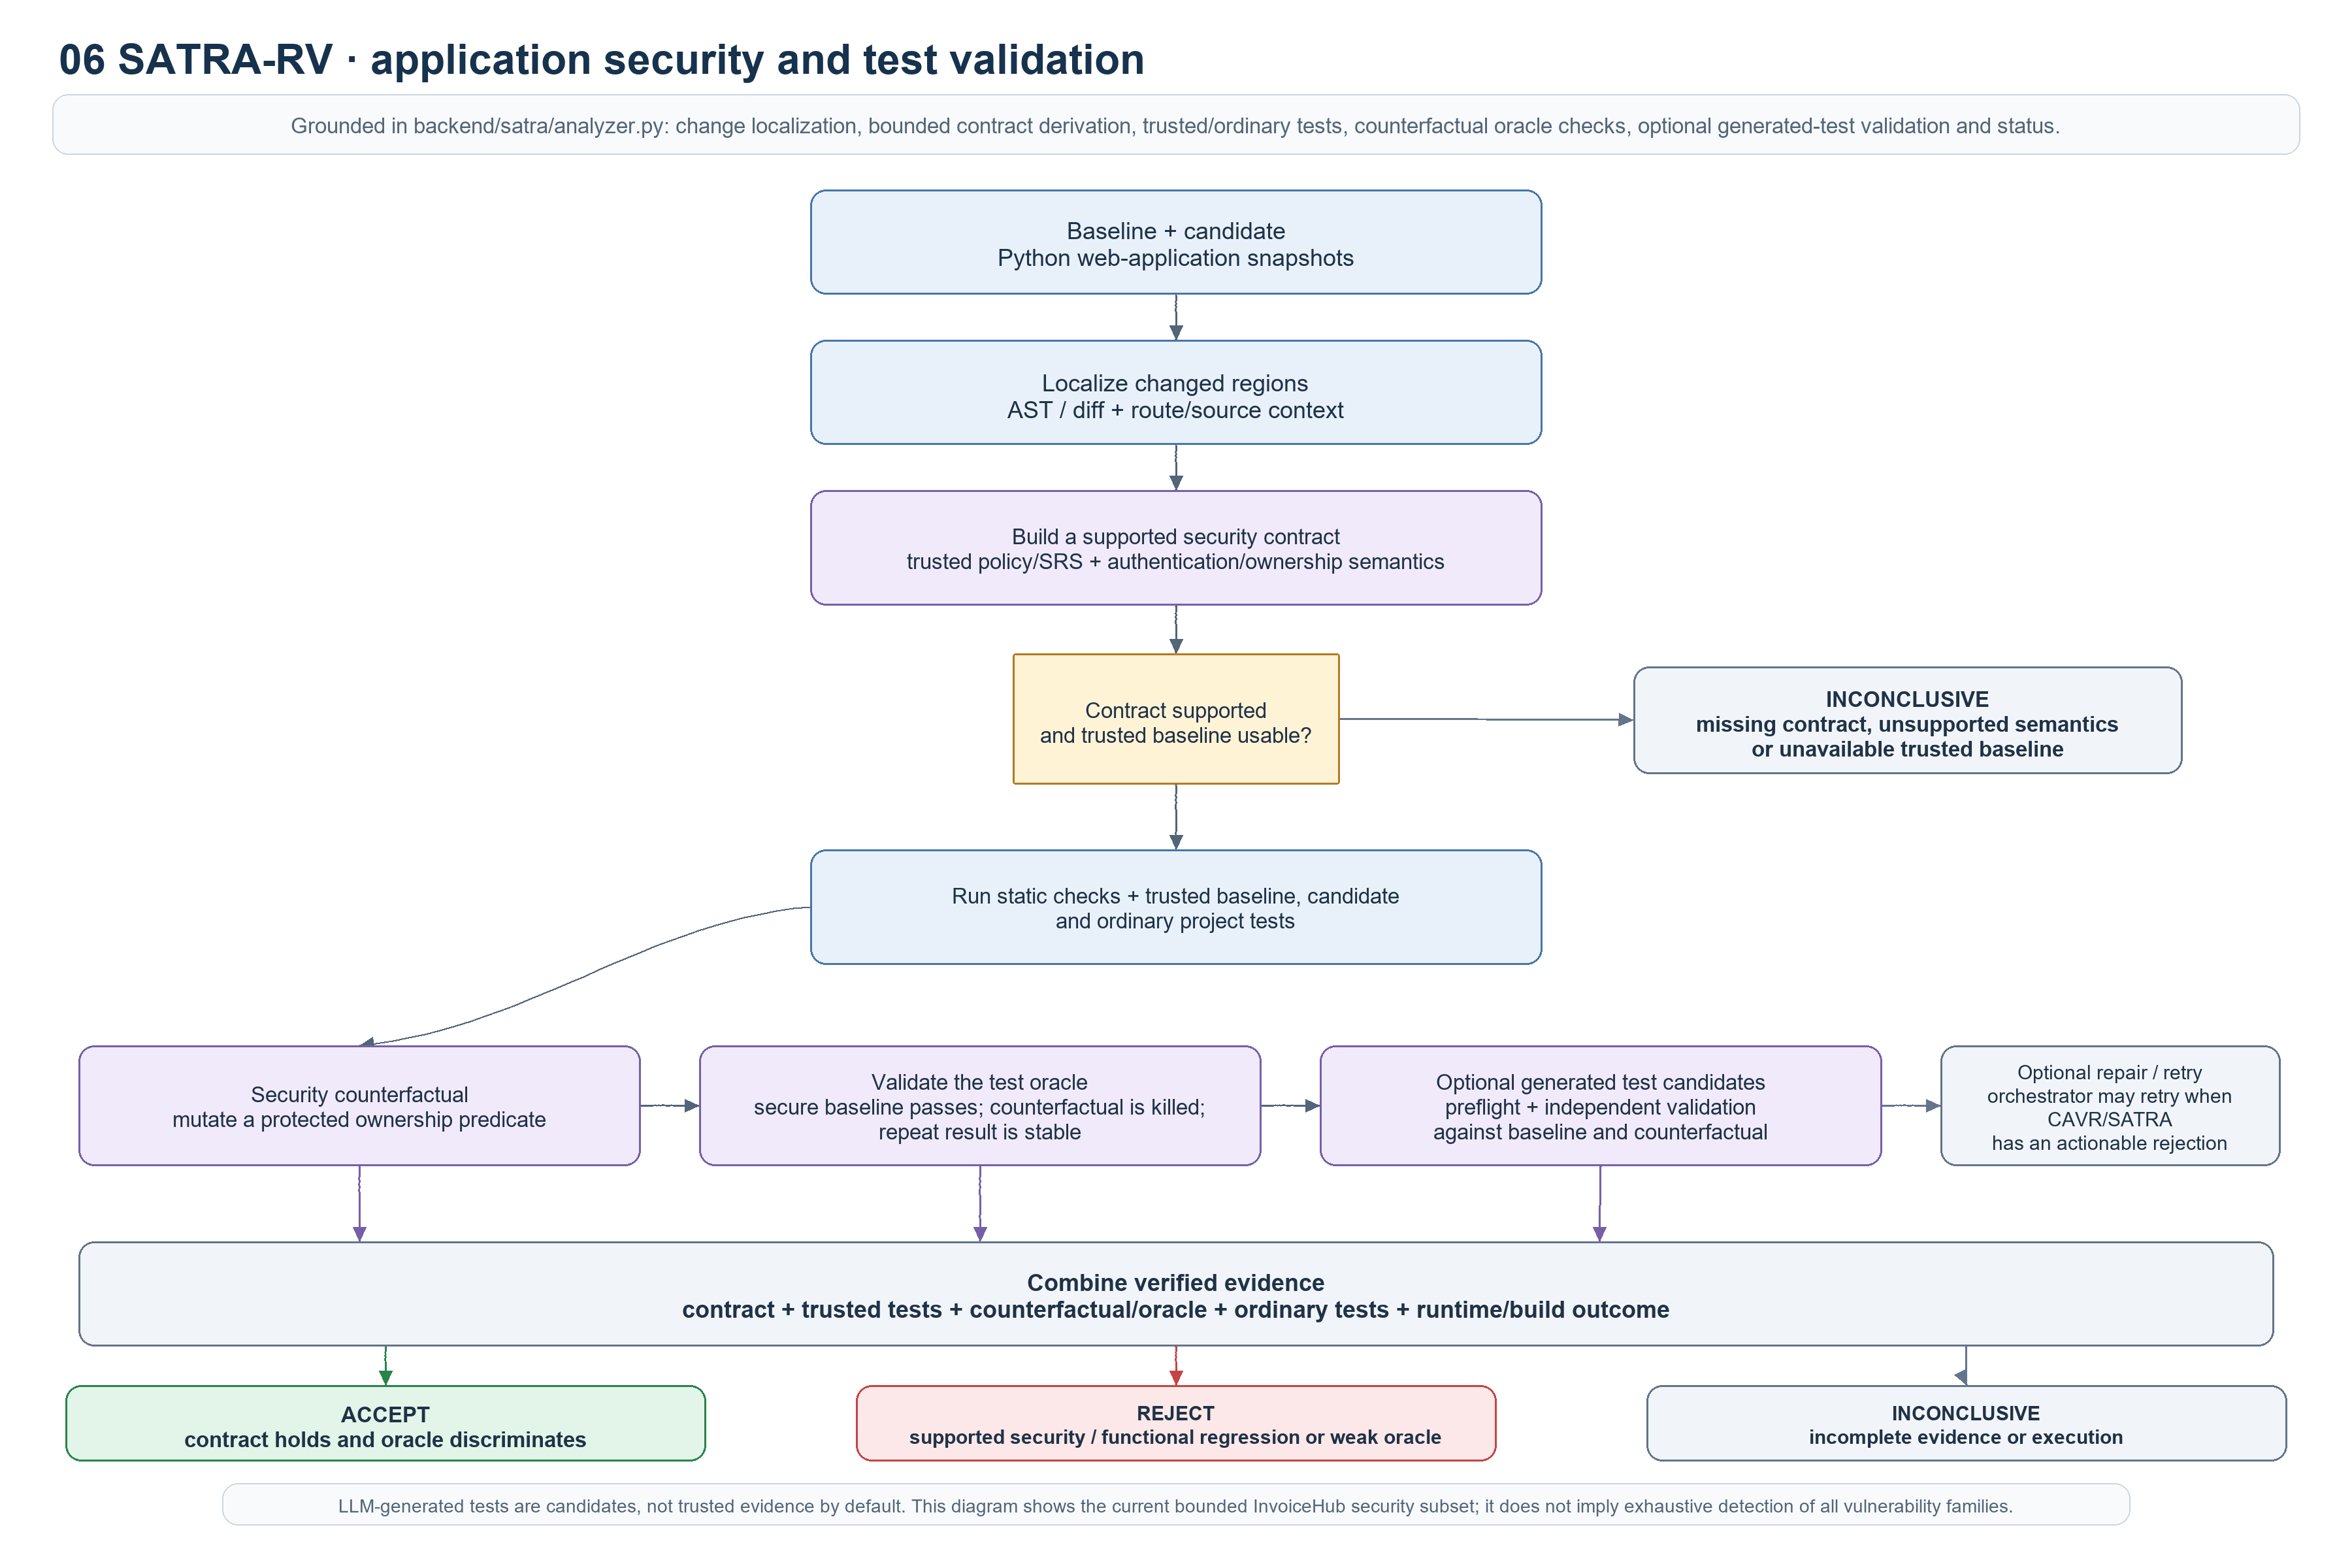
\includegraphics[width=\textheight,height=0.78\textwidth,keepaspectratio]{figures/asent/satra-assurance-flow.png}
\caption{SATRA-RV analysis path from paired source snapshots to an evidence-based result. The diagram is rendered from page 06 of the editable diagrams.net source; generated test candidates are untrusted until validated.}
\label{fig:satra-assurance-flow}
\end{figure}

\begin{figure}[htbp]
\centering
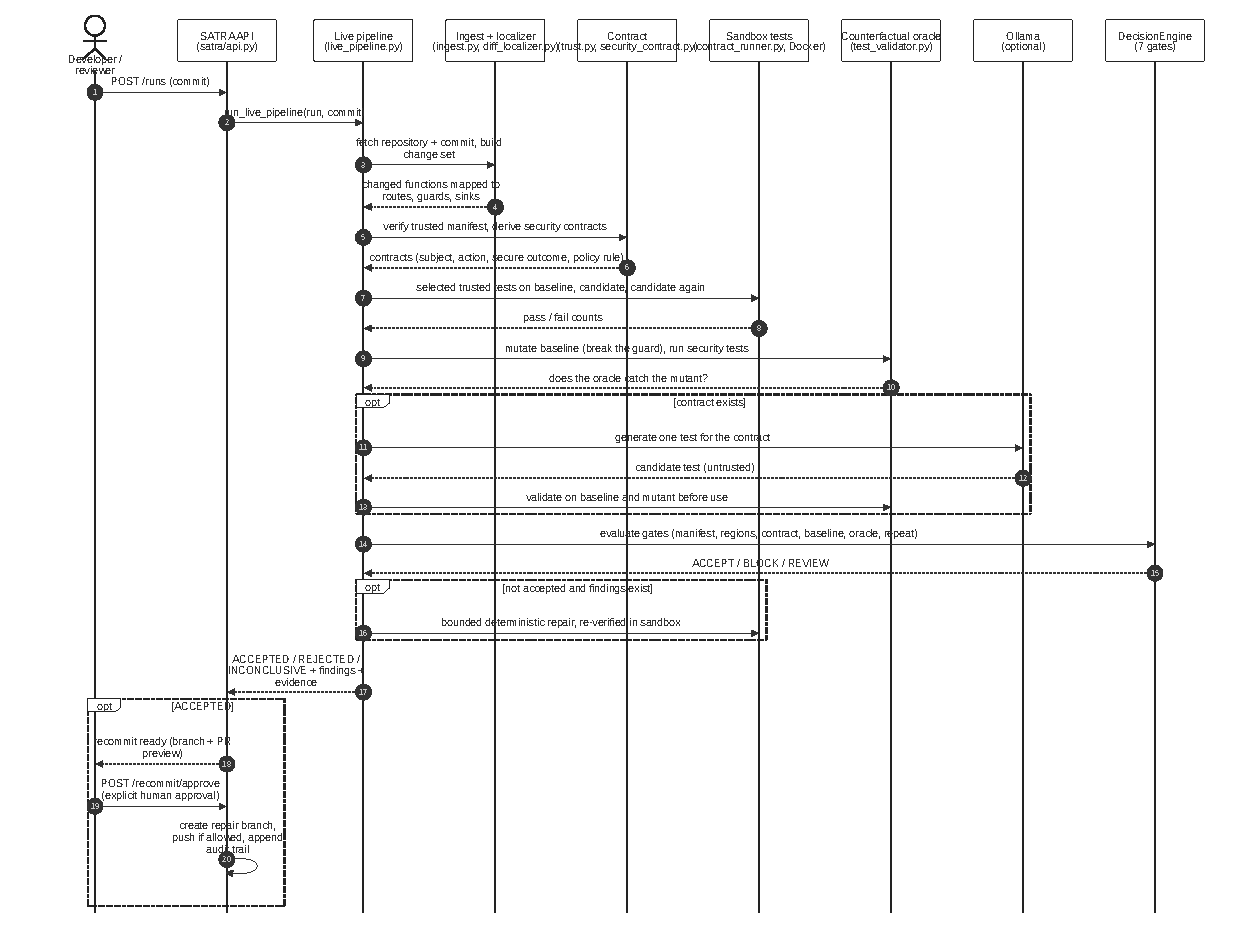
\includegraphics[width=\textwidth]{figures/diagrams/satra-sequence.pdf}
\caption{Sequence of a SATRA-RV live run (\texttt{backend/satra/live\_pipeline.py}) from commit ingestion to the decision and the human-approved recommit.}
\label{fig:satra-sequence}
\end{figure}

\begin{figure}[htbp]
\centering
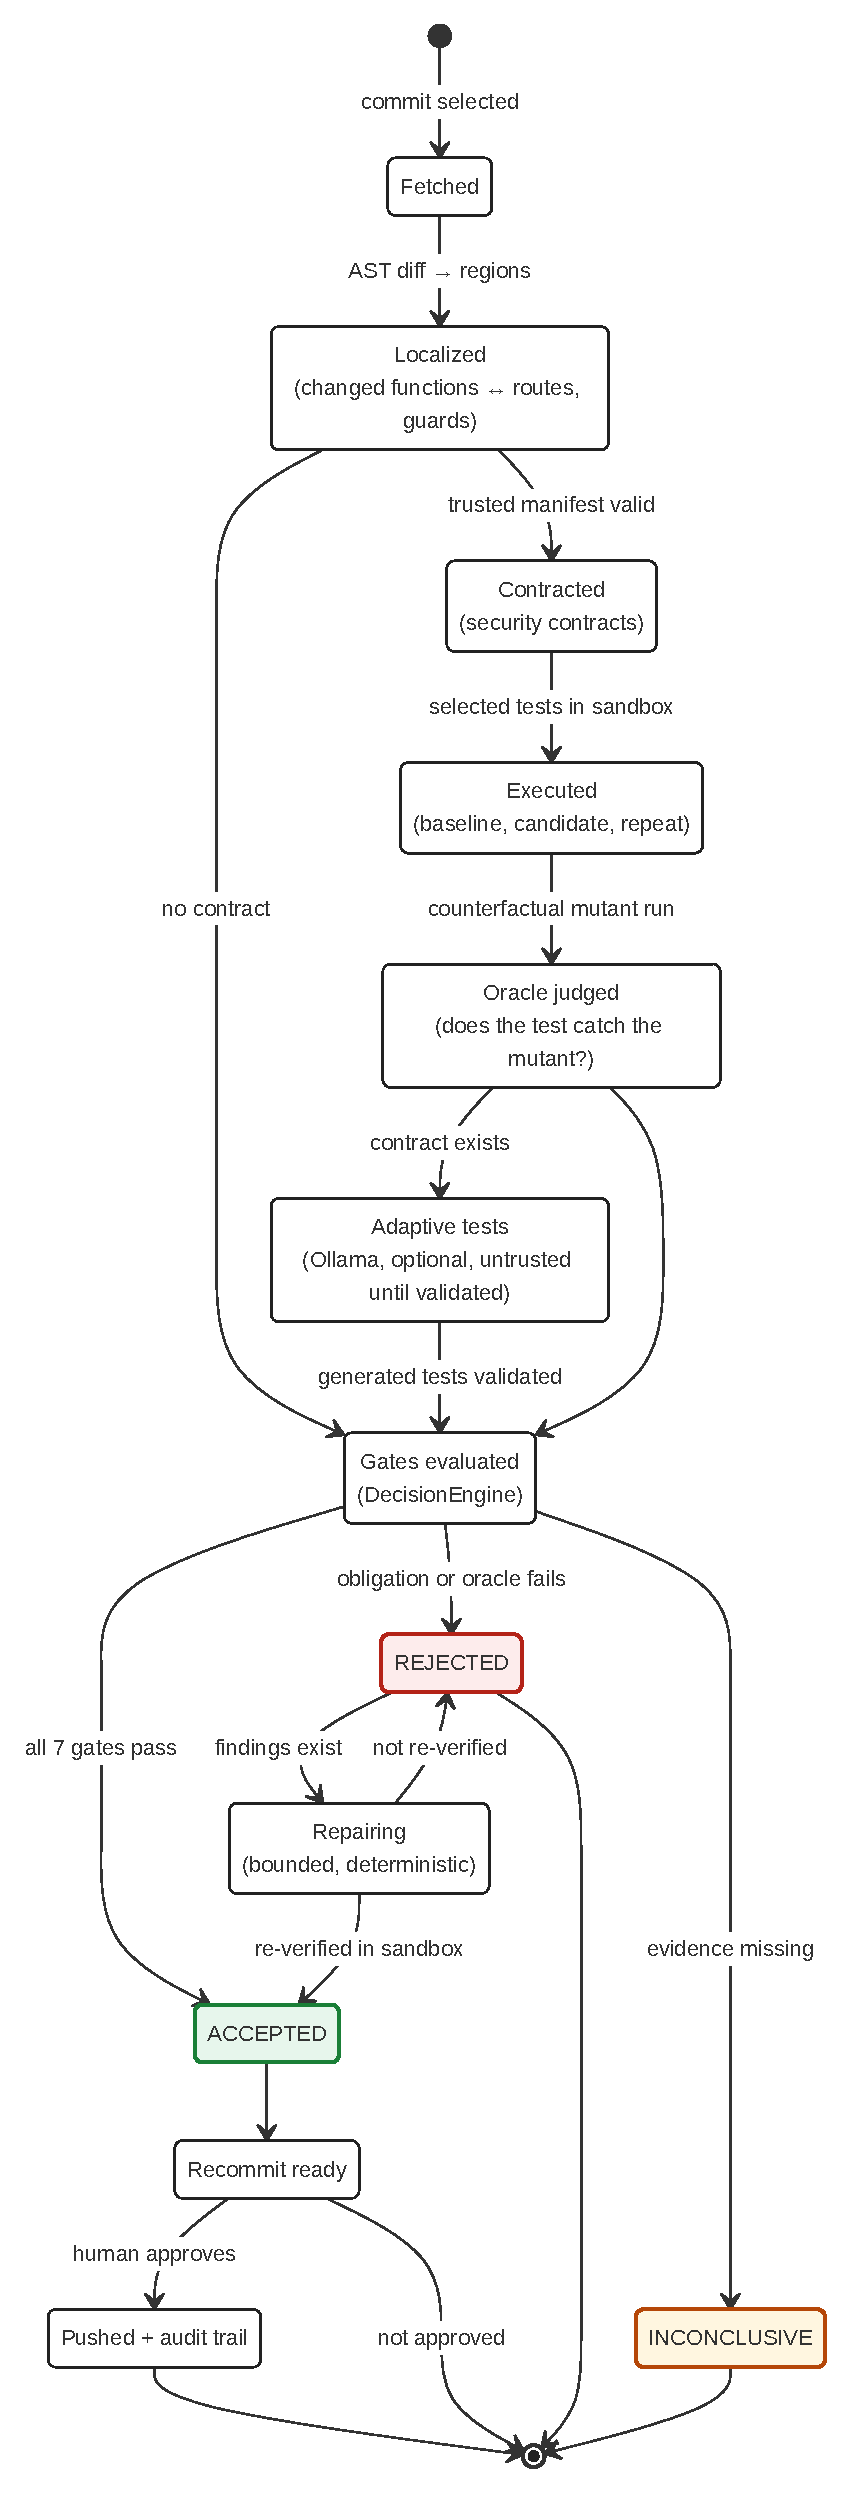
\includegraphics[height=0.8\textheight]{figures/diagrams/satra-state.pdf}
\caption{States of a SATRA-RV run. A repair is only accepted after re-verification in the sandbox, and a recommit is only pushed after explicit human approval.}
\label{fig:satra-state}
\end{figure}

Figures~\ref{fig:satra-sequence} and~\ref{fig:satra-state} show how SATRA-RV judges an application-code change. The commit is fetched and its changed functions are mapped to routes, guards and sinks by AST localization. Security contracts are derived only when the trusted manifest is valid, and the selected trusted tests run in the sandbox on the baseline, the candidate and the candidate again. The counterfactual oracle deliberately breaks the guard in a copy of the baseline and checks that the security tests catch it, so a weak test cannot produce a false pass. Tests generated by Ollama are optional and untrusted until they pass the same validation. The decision engine evaluates seven gates and gives \texttt{ACCEPTED}, \texttt{REJECTED} or \texttt{INCONCLUSIVE}; a rejected run with findings may receive a bounded deterministic repair that counts only after re-verification. An accepted repair is offered as a recommit and is pushed only after an explicit human approval, which is recorded in the audit trail.

\subsection{Implemented Features and Components}
\begin{longtable}{p{0.26\textwidth}p{0.65\textwidth}}
\caption{Implemented Features and Components -- supporting table 1}\\
\toprule
\textbf{Component} & \textbf{Implemented responsibility}\\
\midrule
\path{backend/satra/ingest.py} & Validates allowed repository/ref inputs, resolves commits, records the change set, and prepares isolated baseline/candidate worktrees for the dedicated live pipeline.\\
\path{backend/satra/trust.py} and \path{backend/satra/trusted/} & Verifies SHA-256 fingerprints for trusted SRS, policy, pytest configuration, fixtures, and security tests before use.\\
\path{backend/satra/diff_localizer.py}, \path{astscan.py}, \path{security_contract.py} & Localizes changed Python regions and derives a bounded security contract from supported route and trusted-policy semantics.\\
\path{backend/satra/dictionary.py} & Defines nine rule records. Four Tier-1 entries (IDOR, SQL injection, path traversal, and authentication) have trusted executable tests; five additional rules are marked partial and do not have runnable counterfactual tests in this dictionary.\\
\path{backend/satra/analyzer.py}, \path{contract_runner.py}, \path{pytest_runner.py} & The shared SATRA analyzer runs trusted checks on baseline and candidate, ordinary candidate tests, and a controlled ownership counterfactual, then records test results and reasons. The dedicated live pipeline also maps localized security families and selected routes to trusted test families; the runner uses Docker when present, while its bundled-source fallback is not an arbitrary-code sandbox.\\
\path{backend/satra/test_validator.py}, \path{counterfactuals.py} & Preflight checks generated test syntax and vocabulary, evaluate baseline/mutant/repeat outcomes, and classify an assertion failure separately from an infrastructure error.\\
\path{backend/satra/live_pipeline.py}, \path{ollama_adapter.py} & The dedicated live path can request optional local Ollama test candidates and validate them against the contract and counterfactual; unavailable Ollama is reported as skipped. Model output is not authoritative.\\
\path{backend/satra/decision_engine.py}, \path{repair.py}, \path{repair_inline.py} & The dedicated path evaluates its explicit gate set and may propose bounded deterministic repairs; proposed changes are reported only after re-verification.\\
\path{backend/satra/recommit.py}, \path{audit_trail.py} & Prepare a uniquely named local repair branch with audit metadata, require explicit approval/policy checks before recommit, and maintain a tamper-evident local audit record. This does not establish that a repair was pushed to a production repository.\\
\path{backend/satra/api.py}, \path{frontend/src/components/SatraModule.tsx} & Expose the dedicated SATRA API and React interface, including commit selection, diff, live progress, gate matrix, evidence drawer, and approval interaction.\\
\bottomrule
\end{longtable}

\subsection{Algorithms and Technical Decisions}
The deterministic checks start from a baseline/candidate pair rather than treating a green candidate test suite as sufficient. The localizer associates changed syntax with security-relevant functions and routes. A contract is formed only when the configured trusted policy and supported application semantics provide authority. The trusted tests are run against both sides; the candidate is also checked by its ordinary tests. For the ownership rule, SATRA applies a supported AST counterfactual that removes the ownership guard and checks whether the security oracle rejects it. The validator requires a passing secure baseline, a killed counterfactual, and a repeatable result; execution errors are not classified as successful mutant kills.

The shared analyzer and dedicated live pipeline have distinct status policies and integrations. In the shared route, the bounded analyzer reports \texttt{ACCEPT}, \texttt{REJECT}, or \texttt{INCONCLUSIVE}; the ASENT final gate then checks that applicable evidence is current, integrity-valid, and bound to the same candidate snapshot and module input. The dedicated live pipeline additionally exposes its SATRA gate progression and optional local Ollama stage. Neither path treats generated text as proof. SATRA's module result and ASENT's shared result must therefore be reported separately.

The security dictionary is not uniformly executable. Its four full rules are supported by trusted tests, while the command-injection, insecure-deserialization, SSRF, XSS, and CSRF entries are partial/static or template-level records. The implementation and its UI expose this difference rather than claiming complete detection. Requirements and test names are listed in Chapter~4 and the source test inventory at \path{docs/satra/test-inventory.md}.

The later dedicated live-pipeline update at master commits \texttt{e875904} and \texttt{dfd70d4} adds PR-aware test selection in \path{backend/satra/contract_runner.py}. The selector maps localized security-family identifiers to trusted test files, uses a small route-name fallback when no family is selected, and falls back to the full trusted suite when no test is mapped. It emits a per-family selection reason for the UI. This is bounded prioritization over the available rule and route labels, not complete call-graph reachability. Pruned families are marked as pruned in the result and counted separately, but are not actually executed; no dedicated unit test for the selection mapping was found in the current test tree. Current-master CI passed at \texttt{dfd70d4}; the report therefore records the feature and its limits without presenting the earlier PR~\#5 SATRA test count as specific proof of the selector.

\subsection{Programming Style, Tools, and Technologies}
The implementation uses both procedural and object-oriented programming. Most analyzer stages, AST operations, rule loading, and test evaluation are module-level functions. Object-oriented structures are used where state and interfaces are useful, including Pydantic request/data models, the \texttt{DecisionEngine}, the local Ollama client, and API/service helpers. The React UI is implemented with functional components and hooks. It would be inaccurate to describe the project as exclusively object-oriented or exclusively procedural.

The code uses Python, FastAPI, Pydantic, pytest, Python's AST facilities, Git worktrees, Docker/Podman where available, and a React/TypeScript frontend. Ollama is optional and local to the developer environment; it is not required for the deterministic shared analyzer. CI runs Python 3.12 on Ubuntu and explicitly builds/verifies the SATRA sandbox before the Docker-dependent cases.

\subsection{Demonstration Evidence and Limits}
The integrated source was merged through PR~\#5 at exact tested head \texttt{554b6d51ac\allowbreak{}ca29f99c39\allowbreak{}6c30403620\allowbreak{}15ee460262} (merge \texttt{ffe8aa91}). The SATRA CI run \href{https://github.com/SheharyarAli-Dev/Working-POC/actions/runs/38260995764}{38260995764} and Core CI run \href{https://github.com/SheharyarAli-Dev/Working-POC/actions/runs/38260995652}{38260995652} succeeded on that exact head. The SATRA workflow ran its focused suite and four required Docker sandbox checks; Chapter~7 gives the counts and scope. Later commits \texttt{e875904} and \texttt{dfd70d4} update the dedicated live pipeline and UI. They passed current-master CI runs \href{https://github.com/SheharyarAli-Dev/Working-POC/actions/runs/38540057836}{38540057836} and \href{https://github.com/SheharyarAli-Dev/Working-POC/actions/runs/38542552735}{38542552735}. These later runs establish the recorded repository checks on their exact heads; they do not replace the exact-head PR~\#5 SATRA and Docker-specific counts, or establish isolated test coverage for the new selector.

The repository contains a dedicated SATRA frontend and a recorded defense replay, but this report does not treat a replay as a fresh live run. Fresh completed SATRA-specific browser screenshots and independently reviewed run outputs are not present in the report evidence directory. The integrated Run Workflow rehearsals are SABLE-focused and record SATRA as \texttt{INCONCLUSIVE} on the native-Windows host; they demonstrate the shared gate's handling of that status, not a successful SATRA acceptance. No live cloud deployment is claimed. The source design and test report also leave comparative research, independent benchmark validity, and production-scale detection rates as future work.


\section{Iteration Outcome}

SABLE milestones I1--I4 are implemented for the bounded mid-evaluation model (Chapter 4; Appendix A). The unresolved-role-binding correction from \texttt{58b0a3d} is present in the verified combined snapshot \texttt{665b224} on \texttt{integration/sable-satra-cavr}. The initial focused CI result was 44 passed on \texttt{9a4dc3d}; the later correction-containing local selection was 27 passed with 10 deselected; the focused shared-assurance job on the combined snapshot was 46 passed. The integrated implementation is isolated from \texttt{master} pending team review.

\chapter{Testing and Early Validation}
\begin{sloppypar}
Testing at the FYP-1 Mid stage checks whether the implemented modules follow their stated rules on controlled inputs and whether the shared gate consumes current evidence safely. This report separates module tests, combined CI, and live UI demonstration evidence. It does not claim live AWS validation or independent evaluation on production Terraform.
\end{sloppypar}

\section{Integrated CI: Verified Mid-Evaluation Snapshot}
The combined implementation source snapshot is commit \texttt{84f91a9} on \texttt{integration/sable-satra-cavr}. Its post-fix CI runs succeeded:
\begin{itemize}
    \item \textbf{Core CI, run 38220597702:} all jobs succeeded; the no-container full-suite artifact recorded 1,428 passed, 30 skipped, 0 failed, and 0 errors. Its separate frontend-render job passed 26 cases and the production build succeeded. \href{https://github.com/SheharyarAli-Dev/Working-POC/actions/runs/38220597702}{run link}.
    \item \textbf{SATRA CI, run 38220597564:} 84 SATRA tests passed; all four required Docker sandbox checks ran without skips. The Docker-enabled full suite recorded 1,432 passed, 26 skipped, 0 failed, and 0 errors. \href{https://github.com/SheharyarAli-Dev/Working-POC/actions/runs/38220597564}{run link}.
    \item \textbf{SABLE shared assurance, run 38220597576:} 48 focused tests passed. \href{https://github.com/SheharyarAli-Dev/Working-POC/actions/runs/38220597576}{run link}.
\end{itemize}
The 26 skips in the Docker-enabled broad suite comprise 19 frontend-render cases not run in that job and seven opt-in live-network tests. The separate Core CI full-suite job recorded 30 skipped; frontend rendering ran separately in its dedicated job. The local Windows full suite recorded 1,400 passed, 36 failed, 10 skipped, and 12 setup errors (one warning); these failures/errors were not treated as passes. The local Windows Docker engine could not be started, while Docker-backed CI succeeded on its Linux runner. None of these results means every test ran or that a live AWS deployment was exercised.

PR \#5 was merged normally into \texttt{master}. Its exact tested head was \texttt{554b6d51ac\allowbreak{}ca29f99c39\allowbreak{}6c30403620\allowbreak{}15ee460262}; the merge commit is \texttt{ffe8aa91ca\allowbreak{}89702e5db6\allowbreak{}5b8f7ff129\allowbreak{}aa72f761cc}. All 18 checks passed on the exact PR head. Representative successful workflows are \href{https://github.com/SheharyarAli-Dev/Working-POC/actions/runs/38260995652}{Core CI run 38260995652}, \href{https://github.com/SheharyarAli-Dev/Working-POC/actions/runs/38260995764}{SATRA CI run 38260995764}, and \href{https://github.com/SheharyarAli-Dev/Working-POC/actions/runs/38260995657}{SABLE shared assurance run 38260995657}. The run totals above belong to the separately identified source commit \texttt{84f91a9}; they are not inferred from these exact-head checks. Formal branch protection was not enabled at the last repository check.

The post-merge \href{https://github.com/SheharyarAli-Dev/Working-POC/actions/runs/38262089770}{CD run 38262089770} on \texttt{ffe8aa91} successfully built and published the Docker image and passed its image smoke test; the tag-only release job was skipped. This establishes registry publication and image smoke behavior only, not a persistent production-host or AWS/Terraform deployment. The repository had no enabled branch protection or ruleset at the last check.

\section{Testing Strategy}
The local focused selection combines SABLE unit and fixture tests, the ground-truth isolation check, and the shared integration test. Cases include expected positive behavior, known wrong-target/weakening regressions, uncertainty at unsupported or ambiguous boundaries, and evidence binding/final-gate outcomes. The authored scenario fixtures are controlled test data rather than an independently sampled dataset.

\section{Test Levels and Techniques}
\begin{itemize}
    \item \textbf{Unit and scenario tests:} parse fixture Terraform, check baseline obligations, rank successors, and assert module verdicts.
    \item \textbf{Regression tests:} compare standalone and shared authorization behavior for unresolved role bindings and explicitly unrelated static roles.
    \item \textbf{Isolation test:} checks the SABLE decision path remains separate from benchmark ground-truth labels.
    \item \textbf{Shared integration test:} runs four shared \texttt{sable\_*} scenarios and asserts published SABLE evidence, candidate snapshot, SABLE input hash, integrity, and final decision.
    \item \textbf{CI evidence:} the initial SABLE-focused CI passed 44 tests on commit \texttt{9a4dc3d}; later shared-assurance CI passed 48 tests on source commit \texttt{84f91a9}. All 18 check runs succeeded on exact merged PR head \texttt{554b6d5}. These are distinct results; the source-run totals and full-suite skips are recorded above.
\end{itemize}

\section{Test Cases}
\setlength{\tabcolsep}{3pt}
\begin{longtable}{p{0.26\textwidth}p{0.49\textwidth}p{0.17\textwidth}}
\caption{Test Cases -- supporting table 1}\\
\toprule
\textbf{Test area / name} & \textbf{Expected result} & \textbf{Result}\\
\midrule
\path{test_sable_real_hcl} & Supported preserved fixtures return \texttt{PRESERVED}; regressed and widened fixtures return \texttt{REGRESSED}; the uncertain fixture returns \texttt{UNKNOWN}. & Passed\\
\path{test_sable_refactor_and_correspondence_cases} & Supported rename/move cases preserve; wrong target and weakened action regress; replacement and competing successors remain unknown. & Passed\\
Unsupported/unknown tests & Unsupported forms, unresolved bindings, and unverified baseline yield \texttt{UNKNOWN}. & Passed\\
Authorization evaluator regression tests & Unresolved dynamic role binding is unknown in both evaluators; a statically known unrelated role does not invalidate the protected role's result. & Passed\\
\path{test_shared_sable_evidence_drives_final_gate} & \texttt{sable\_preserved}: \texttt{PRESERVED}/\texttt{ACCEPT}; \texttt{sable\_regressed}: \texttt{REGRESSED}/\texttt{BLOCK}; \texttt{sable\_unknown} and unresolved binding: \texttt{UNKNOWN}/\texttt{REVIEW}. Evidence bindings and integrity also assert. & 4 cases passed\\
\path{test_sable_final_gate_rejects_untrusted_evidence} & Stale, mismatched, or integrity-invalid evidence cannot establish acceptance. & Not selected in the reported local command\\
\bottomrule
\end{longtable}
\setlength{\tabcolsep}{6pt}

\section{Test Results}
The exact local command executed from the repository root on the current worktree was:
\begin{quote}\small\ttfamily\sloppy\noindent
\path{.venv\Scripts\python.exe} -m pytest \\
\path{tests/test_modules.py} \path{tests/test_sable_isolation.py} \\
\path{tests/test_integration.py::test_shared_sable_evidence_drives_final_gate} \\
-k sable --basetemp \path{.venv\.pytest_sable_mid_audit_20261011_c} -q
\end{quote}
Observed result: \textbf{27 passed, 10 deselected in 47.26s; exit code 0}. The \texttt{-k sable} filter restricts this command to test names containing \texttt{sable}; ten collected items were deselected. The passing selection covers SABLE parser/scenario, correspondence, obligation and uncertainty behavior, the standalone/shared evaluator regression cases, ground-truth isolation, and all four parameterized shared integration scenarios. It does not represent the complete test suite.

\begin{sloppypar}
The shared integration assertions establish that current SABLE evidence was published for the same candidate snapshot, its recomputed SABLE input hash matched, integrity was valid, and each case had the expected final-gate decision in the test setup. When other modules are applicable, their results also affect the aggregate: the fresh browser runbook records SABLE \texttt{PRESERVED} with overall \texttt{REVIEW} because SATRA was inconclusive, and SABLE \texttt{REGRESSED} with overall \texttt{BLOCK}.
\end{sloppypar}

\begin{sloppypar}
The separate initial GitHub Actions run named \textit{SABLE shared assurance} reported \textbf{44 passed} on commit \path{9a4dc3d94626ec1f14683b7420f4640d97de20c7}. That result predates the unresolved-role-binding correction. The correction was committed as \texttt{58b0a3d}; later baseline and evidence-gate corrections are in source commit \texttt{84f91a9}, whose focused shared-assurance job passed 48 tests. The correction-containing local selection reported above (27 passed, 10 deselected) was another distinct run. All 18 checks then succeeded on exact PR head \texttt{554b6d5}, which was merged as \texttt{ffe8aa9}. None of these results establishes complete Terraform/AWS semantics or live-cloud behavior.
\end{sloppypar}

% Module test sections (each owned by its member, see OWNERS.md)
% OWNER: Maryam Fatima
\section{CAVR Testing}
\subsection{Test Cases}
% Table: Test ID | Purpose | Input | Expected | Result
\subsection{Test Results}
\subsection{Edge and Failure Cases}
\subsection{Defects and Corrective Actions}
\subsection{Current Validation Status}

\section{SATRA-RV Testing}
\label{sec:satra-testing}

\subsection{Test Cases and Expected Outcomes}
The selected tests verify bounded implementation behaviors. The names below are from \path{tests/test_satra*.py} and the SATRA workflow selection; they are not a claim that every possible vulnerability family or application framework is tested.

\begin{longtable}{p{0.24\textwidth}p{0.48\textwidth}p{0.18\textwidth}}
\toprule
\textbf{Test area / representative test} & \textbf{Expected behavior} & \textbf{Recorded result}\\
\midrule
\endfirsthead
\toprule
\textbf{Test area / representative test} & \textbf{Expected behavior} & \textbf{Recorded result}\\
\midrule
\endhead
Commit ingestion: \path{test_satra_ingest.py} & Accept valid refs from the allowlisted repository; reject malformed SHAs/refs and unapproved URLs; preserve add/delete/rename and merge-parent behavior. & SATRA CI passed\\
Trusted manifest: \path{test_satra_trust_and_seed.py} & Detect modified, deleted, missing, or planted trusted files; preserve normalized line-ending fingerprints and refuse unsafe reseeding. & SATRA CI passed\\
Localization and contract: \path{test_satra_localize.py}, \path{test_satra_rule_contract.py} & Localize security-relevant edits; keep unsupported or authority-free contract cases inconclusive. & SATRA CI passed\\
Dictionary and counterfactual: \path{test_satra_dictionary.py}, \path{test_satra_counterfactuals.py} & Check registered supported rules, synthesize the supported ownership mutation, and distinguish a weakened oracle from a genuine assertion kill. & SATRA CI passed\\
Sandbox: \path{test_satra_sandbox.py} & Enforce network isolation, read-only root, temporary storage, and execution timeout in the container-backed checks. & 4 required checks ran without skips in SATRA CI\\
Validator and gate: \path{test_satra_ollama_and_validator.py}, \path{test_satra_decision_and_repair.py} & Reject malformed, vacuous, weakened, or misaligned tests; classify errors separately from assertion failures; evaluate the gate and evidence bundle. & SATRA CI passed\\
API and live path: \path{test_satra_live_pipeline.py} & Refuse untrusted host execution without an allowed backend and exercise the real pipeline through completion with non-simulated evidence. & SATRA CI passed\\
Recommit/audit: \path{test_satra_recommit.py} & Require approval/policy checks, create unique local repair branches, and detect tampering of the append-only audit record. & SATRA CI passed\\
\bottomrule
\end{longtable}

\subsection{CI Results and Provenance}
The latest verified SATRA-specific workflow record used here is SATRA CI run \href{https://github.com/SheharyarAli-Dev/Working-POC/actions/runs/38260995764}{38260995764} on exact PR~\#5 head \texttt{554b6d51acca29f99c396c3040362015ee460262}. The workflow reported 84 SATRA tests passed and required the four Docker sandbox tests to be present and unskipped. Its Docker-enabled full-suite job recorded 1,432 passed, 26 skipped, zero failures, and zero errors. Skips included tests intentionally belonging to a separate frontend-render job and opt-in network cases; the result is not a claim that every project test ran in this job. The separate Core CI run \href{https://github.com/SheharyarAli-Dev/Working-POC/actions/runs/38260995652}{38260995652} passed the production frontend build and its 26 component-render checks. All 18 PR checks passed on the exact PR head before normal merge as \texttt{ffe8aa91}.

The subsequent `origin/master` changes through report commit \texttt{b16b48409a9ddceecc76d49d6cceaf5846511432} add report material and workflow/report provenance; they do not modify SATRA implementation files. The counts above therefore remain provenance for the unchanged SATRA source snapshot at \texttt{554b6d5}, not a newly executed test run on the report commit. A new report workflow verifies the report artifact only and is not SATRA CI.

An older SATRA source report documents 83 passed tests on commit \texttt{02953a4}; that earlier count is not used as the current integrated result. Historical totals are retained only when their source commit is named.

\subsection{Failure Cases, Defects, and Limitations}
The tests exercise invalid commit inputs, damaged trusted authority, missing contracts, weakened or vacuous assertions, mutation survival, execution errors, missing Docker, recommit branch collisions, and audit tampering. These establish behavior for their checked cases. They do not prove that every security defect will be found or every generated test will be sound.

On the native Windows workstation, the recorded full-suite run had 1,400 passed, 36 failed, 10 skipped, and 12 setup errors. These failures and errors are not recast as successful tests. The local Docker engine and pinned Linux sandbox could not be started there; the sandbox evidence cited above comes from the Ubuntu CI run where Docker was built and required checks ran. The current implementation is bounded to the supported Python/InvoiceHub contracts, partial dictionary entries remain partial, and independent comparative research is not complete.

No fresh SATRA-specific browser run was captured for this report pass. The retained shared Run Workflow scenarios exercised SABLE and reported SATRA as \texttt{INCONCLUSIVE} on Windows; these are evidence that the shared gate keeps uncertainty visible, not successful SATRA acceptance results. The dedicated SATRA page and recorded replay are described in Chapter~6, but are not substituted for a fresh live test result.

\subsection{Current Validation Status}
\begin{itemize}
    \item \textbf{Verified by the exact-head CI record:} 84 focused SATRA tests passed; all four required Docker sandbox cases ran without skips; the Docker-enabled broad suite reported 1,432 passed, 26 skipped, zero failures, and zero errors.
    \item \textbf{Verified by separate Core CI:} frontend production build and 26 component-render checks passed on exact PR head \texttt{554b6d5}.
    \item \textbf{Verified by integrated pull-request checks:} all 18 checks succeeded on exact PR head \texttt{554b6d5}; this is a CI record, not a new local execution for this report edit.
    \item \textbf{Not verified here:} a fresh browser-captured SATRA success case; broad language/framework coverage; all dictionary families at runnable depth; production-scale performance; a live cloud deployment; or comparative research advantage.
\end{itemize}


\section{Acceptance Testing / Validation}
\begin{sloppypar}
For the supported model, a \texttt{PRESERVED} verdict requires a verified baseline, a supported unique successor, and the registered principal/action/resource predicate holding on that successor. A supported known wrong-target or weakened-action case returns \texttt{REGRESSED}. Unresolved role binding, unsupported policy semantics, invalid baseline, or ambiguous correspondence returns \texttt{UNKNOWN}. In the shared gate, current integrity-valid SABLE evidence maps those three statuses to \texttt{ACCEPT}, \texttt{BLOCK}, and \texttt{REVIEW} respectively, subject to other applicable modules.
\end{sloppypar}

\begin{sloppypar}
The retained integrated application capture documents a separate shared run \texttt{104074afe883}: CAVR \texttt{VERIFIED}, SABLE \texttt{REGRESSED}, SATRA \texttt{INCONCLUSIVE}, overall \texttt{BLOCK}. The dedicated SABLE page captures another wrong-target case. These application captures support the visible demonstrations described in Chapter 9; they do not substitute for the four-case test assertions or demonstrate live cloud behavior.
\end{sloppypar}

\section{Edge and Failure Cases}
The selected fixture tests cover malformed HCL, unsupported module expansion and policy forms, unresolved role attachment, an unverified baseline, absent or competing successor evidence, a wrong policy target, and a weakened required action. In the shared test, evidence is also checked against the current snapshot and module input hash. These tests bound the supported behavior; they do not exhaust the Terraform language or all AWS authorization interactions.

\section{Defects and Corrective Actions}
\begin{sloppypar}
The audit compared \texttt{backend/sable/authorization.py} with \texttt{backend/sable/policy\_semantics.py}. For the required cases, both agree on preserved authorization and known wrong-target/weakening regressions. They differed on an unresolved dynamic inline-policy role binding: the standalone evaluator could ignore it while the shared evaluator classified it as unknown. The standalone path now records that unresolved binding as outside-model evidence and returns an unknown authorization result. The regression tests also check that a binding to a statically known different role is still ignored. This is a narrow correction, not a broad evaluator rewrite.
\end{sloppypar}

\section{Current Validation Status}
\begin{itemize}
    \item \textbf{Verified in local focused selection:} 27 selected tests passed and 10 were deselected; this was not the full suite.
    \item \textbf{Verified in CI:} 44 focused tests passed on initial SABLE commit \texttt{9a4dc3d}; 48 focused shared-assurance tests passed on source commit \texttt{84f91a9}. All 18 check runs succeeded on exact merged PR head \texttt{554b6d5}.
    \item \textbf{Verified in Docker-enabled CI:} SATRA passed 84 tests and the combined full suite recorded 1,432 passed, 26 skipped, 0 failed, and 0 errors; all four required Docker checks ran without skips. Frontend build and 26 render tests passed separately in Core CI.
    \item \textbf{Native Windows full-suite result:} 1,400 passed, 36 failed, 10 skipped, 12 setup errors, and one warning. These are reported as failures/errors; the Windows Docker engine and pinned sandbox runtime were unavailable and Windows/POSIX differences affected other tests.
    \item \textbf{Verified for tested fixtures:} preserved, regressed, and unknown outcomes are differentiated, and four shared final-gate scenarios assert evidence binding and decisions.
    \item \textbf{Not established:} complete Terraform/AWS semantics, live-cloud behavior, independent benchmark validity, production-scale performance, or comparative research advantage. The Windows host did not provide a running Docker engine; Docker-dependent evidence is from CI.
\end{itemize}

The test evidence is early controlled validation. The scenario set is authored in-house; its outcomes are useful as regression checks but are not an independent estimate of real-world error rates.

\chapter{Project Management and Development Evidence}

This chapter records implementation, repository, testing, tool-use, and risk evidence available for the current SABLE branch. Team-wide claims are limited to evidence visible in the shared repository. Contributions for other modules should be reconciled against their own branches and commits before the complete team report is submitted.

\section{Work Completed}

The current SABLE contribution includes a local Terraform/HCL analysis pipeline, a bounded IAM/S3 authorization evaluator, successor correspondence, explicit outcomes of \texttt{PRESERVED}, \texttt{REGRESSED}, and \texttt{UNKNOWN}, baseline comparisons B0--B4, authored scenarios, and integration with the shared evidence/final-gate path. Automated tests cover expected results, unsupported and ambiguous inputs, stale evidence, input-hash mismatch, and evidence integrity. The unresolved-role-binding correction is commit \texttt{58b0a3d}; it is included in verified combined commit \texttt{665b224} on \texttt{integration/sable-satra-cavr}. The 27-pass local audit and 44-pass initial CI results are historical, separate results; the focused shared-assurance CI on the combined snapshot passed 46 tests.

The initial SABLE changes were published on the team's \texttt{sable} branch. The current verification point is the isolated combined branch \texttt{integration/sable-satra-cavr} at \texttt{665b224}; it contains the integrated CAVR, SATRA-RV, SABLE, and shared workflow snapshot. It is not merged into \texttt{master}. The SABLE shared-assurance job on this commit passed 46 tests.

\subsection{Rendered Application Evidence}
The integrated capture below comes from the shared ASENT Run Workflow, not from the dedicated SABLE page. It records run \texttt{104074afe883} for the \texttt{sable\_regressed} storage-refactor scenario. The displayed module outcomes are CAVR \texttt{VERIFIED}, SABLE \texttt{REGRESSED}, and SATRA \texttt{INCONCLUSIVE}, with an overall final decision of \texttt{BLOCK}. The trace shows a known obligation that does not hold and a candidate policy target changed through the storage module. Since SATRA is also inconclusive, the screenshot is not evidence that SABLE was the sole cause of the overall gate result.

\begin{figure}[p]
    \centering
    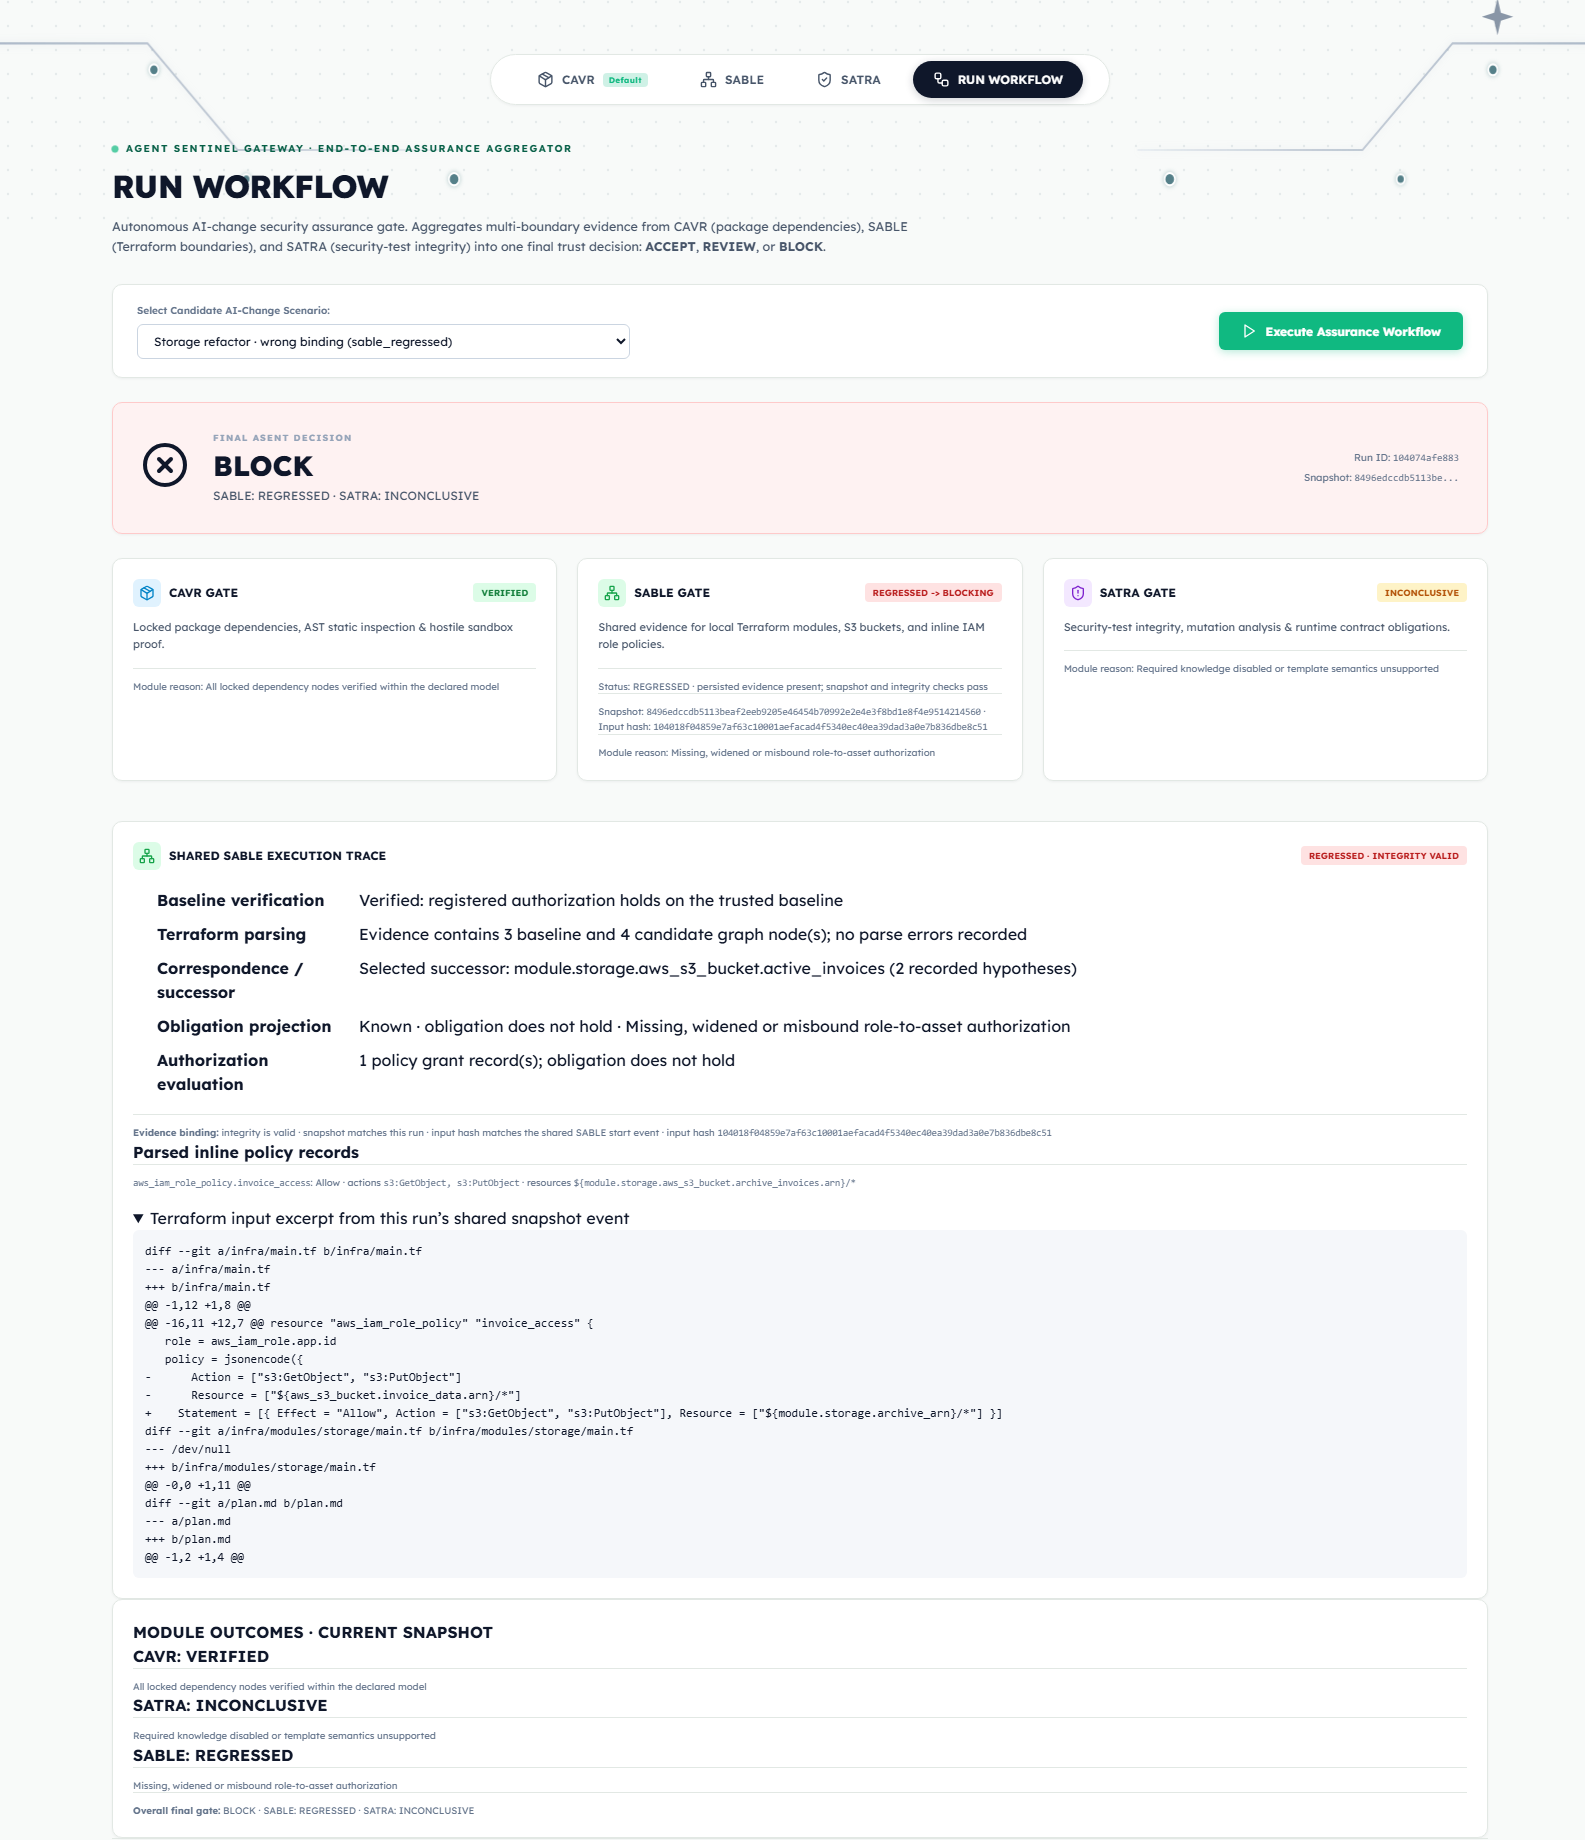
\includegraphics[width=0.98\textwidth,height=0.79\textheight,keepaspectratio]{ThesisFigs/asent_shared_sable_regressed_workflow_detail.png}
    \caption{Integrated ASENT Run Workflow for run \texttt{104074afe883}: shared SABLE evidence, candidate Terraform excerpt, module results, and final-gate decision.}
    \label{fig:asent-shared-sable-regressed}
\end{figure}
\clearpage

A separate capture from the dedicated SABLE page covers the distinct \texttt{policy\_\allowbreak{}rewrite\_\allowbreak{}wrong\_\allowbreak{}target} case and the \texttt{S3-\allowbreak{}APPROLE-\allowbreak{}CUSTOMERDATA} obligation. It is a different scenario from the integrated invoice-storage run above.

\begin{figure}[!htbp]
    \centering
    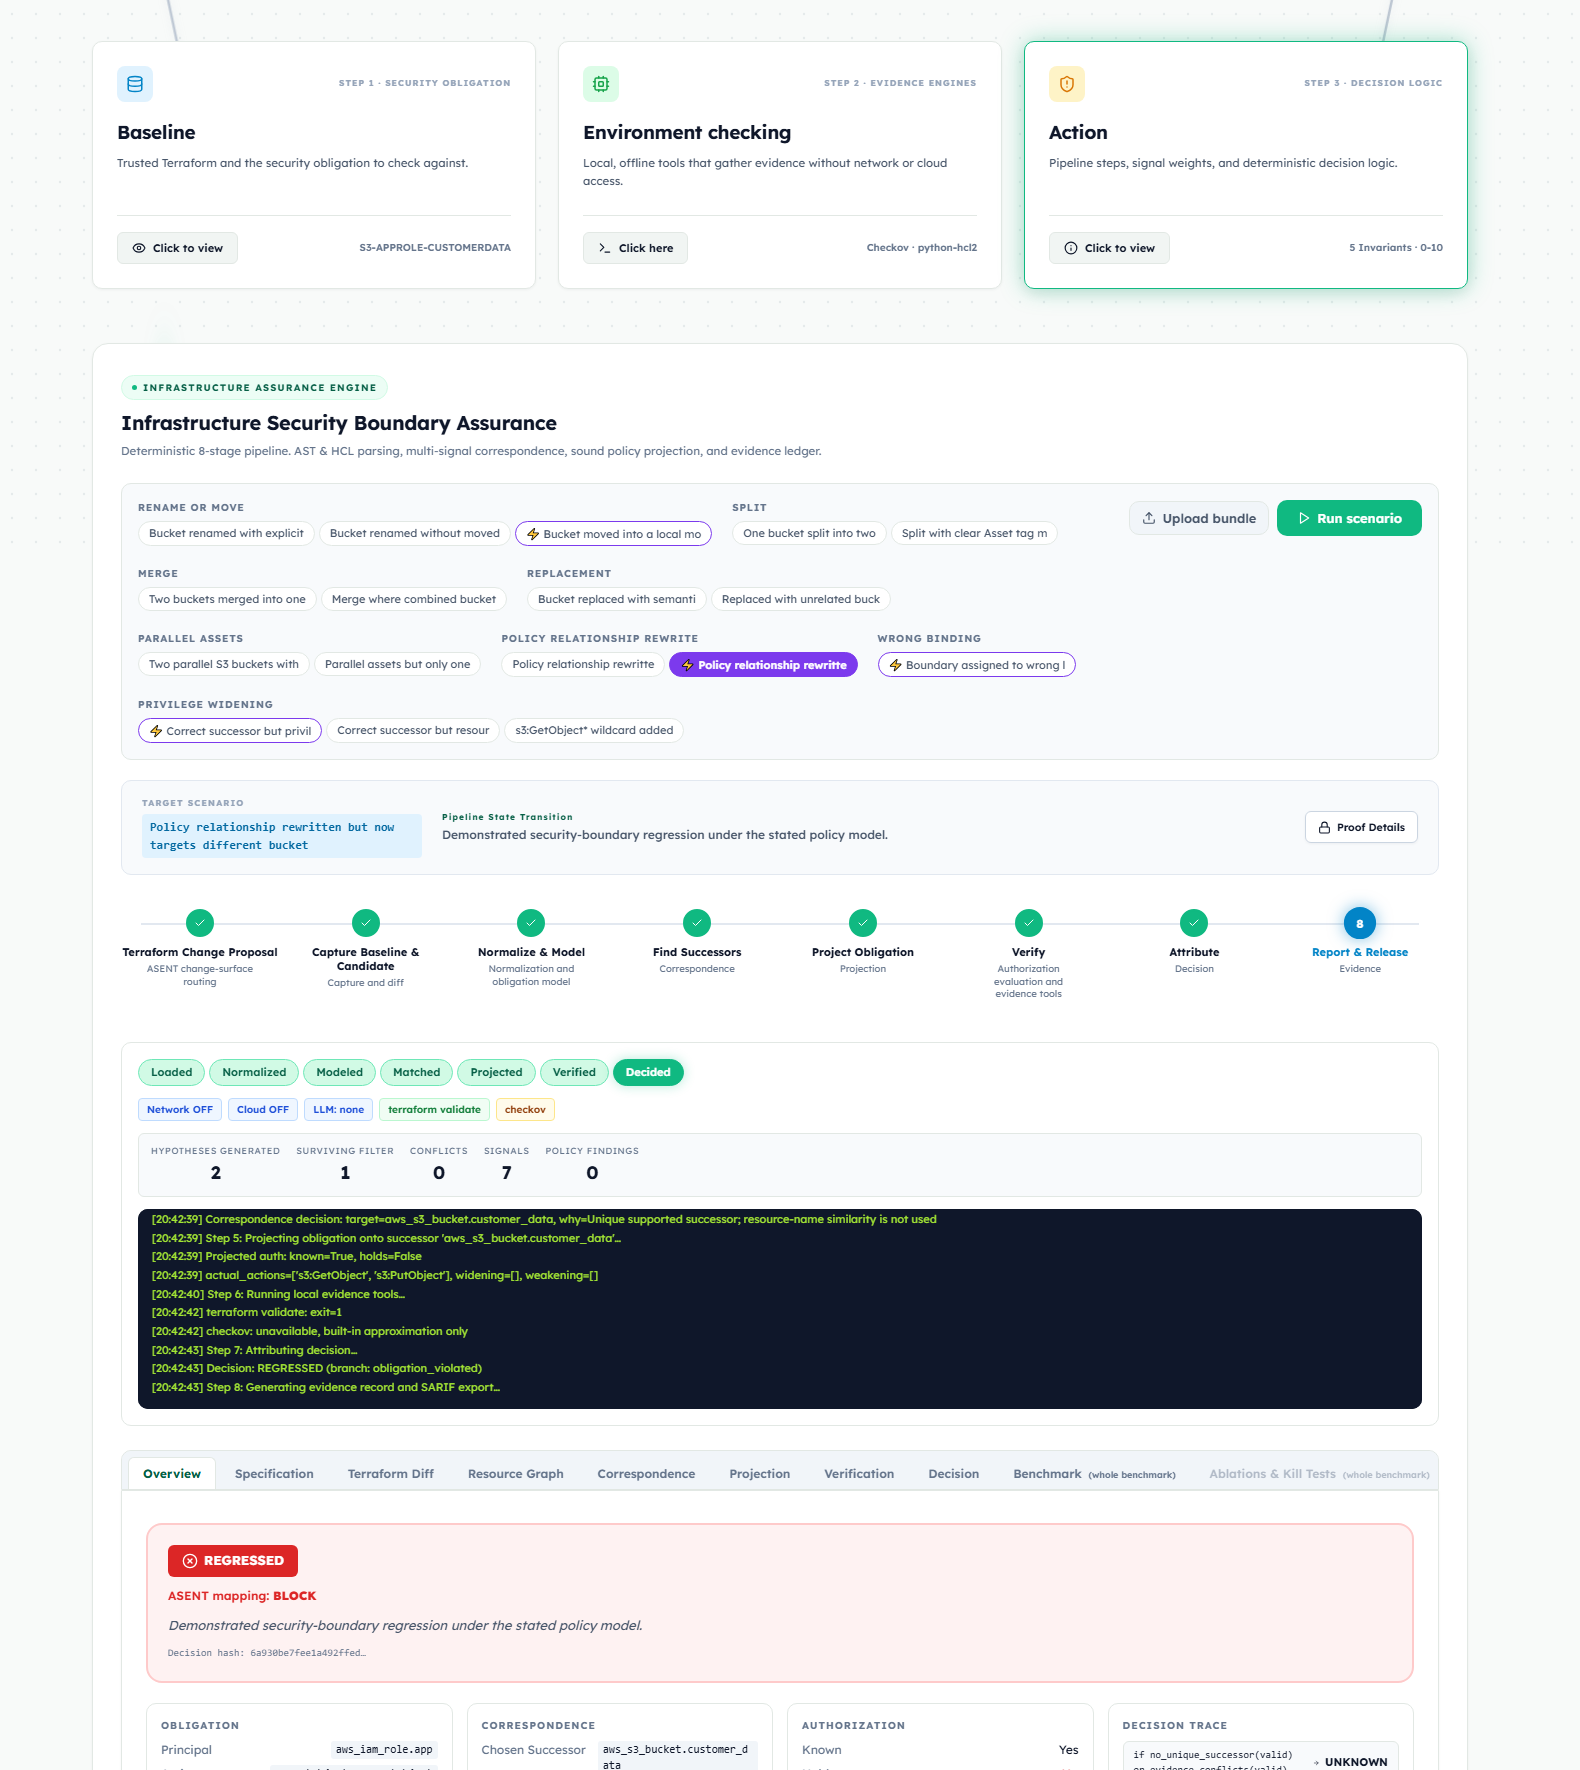
\includegraphics[width=0.96\textwidth,height=0.73\textheight,keepaspectratio]{ThesisFigs/sable_wrong_target_result_detail_crop.png}
    \caption{Dedicated SABLE page: wrong-target scenario result for the \texttt{S3-APPROLE-CUSTOMERDATA} obligation. The UI reports \texttt{REGRESSED}, mapped to \texttt{BLOCK}.}
    \label{fig:sable-customer-data-result}
\end{figure}
\clearpage

\begin{figure}[htbp]
    \centering
    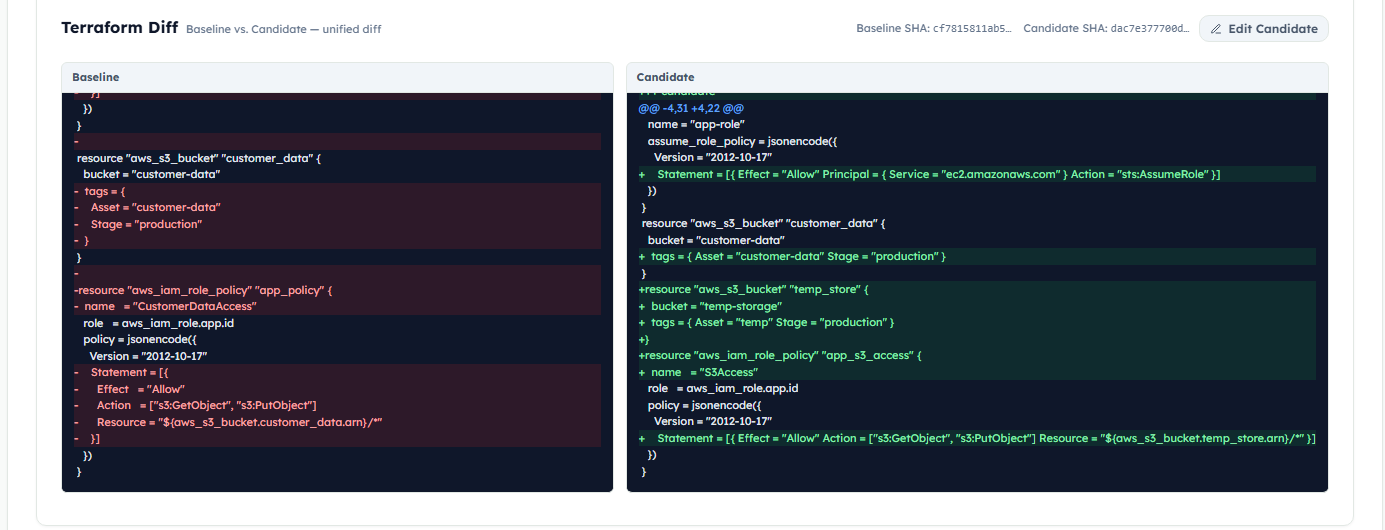
\includegraphics[width=0.99\textwidth,height=0.32\textheight,keepaspectratio]{ThesisFigs/sable_wrong_target_policy_comparison_crop.png}
    \caption{Dedicated SABLE wrong-target scenario: baseline authorization points to the \texttt{customer\_data} bucket, while the candidate policy targets \texttt{temp\_storage}.}
    \label{fig:sable-customer-data-policy-diff}
\end{figure}

The two dedicated-page report figures are focused crops of the saved UI captures; only the visible area was trimmed for readability and the displayed application content was not changed. They support the distinct \texttt{policy\_rewrite\_wrong\_target} scenario, associated with local run \texttt{sable-1791646956750}: the \texttt{S3-APPROLE-CUSTOMERDATA} obligation and policy target change from \texttt{customer\_data} to \texttt{temp\_storage}. These are not screenshots of the integrated invoice-storage run above. None of the screenshots establishes live AWS behavior or applied infrastructure.

\subsection{Earlier Shared-Workflow Rehearsal}
At branch head \texttt{753a55b} on \texttt{sable}, the shared Run Workflow was executed for three mid-evaluation outcomes. These earlier aggregate runs are kept separate from the latest dedicated SABLE module screenshots below. The run records completed with the following module and aggregate decisions:

\small
\setlength{\tabcolsep}{2pt}
\begin{longtable}{p{0.14\textwidth}p{0.15\textwidth}p{0.14\textwidth}p{0.27\textwidth}p{0.16\textwidth}}
\toprule
\textbf{Scenario} & \textbf{Run ID} & \textbf{SABLE} & \textbf{Final gate} & \textbf{Evidence binding}\\
\midrule
\endhead
\path{sable_preserved} & \texttt{b107fd\allowbreak{}8f0f2f} & \texttt{PRESERVED} & \texttt{REVIEW}; SATRA \texttt{INCONCLUSIVE} & Integrity valid; snapshot and input hash match\\
\path{sable_regressed} & \texttt{5c6fe1\allowbreak{}aa3a96} & \texttt{REGRESSED} & \texttt{BLOCK}; SABLE \texttt{REGRESSED}; SATRA \texttt{INCONCLUSIVE} & Integrity valid; snapshot and input hash match\\
\path{sable_unknown} & \texttt{b6d358\allowbreak{}8ec006} & \texttt{UNKNOWN} & \texttt{REVIEW}; SABLE \texttt{UNKNOWN}; SATRA \texttt{INCONCLUSIVE} & Integrity valid; snapshot and input hash match\\
\bottomrule
\end{longtable}
\normalsize
\setlength{\tabcolsep}{6pt}
The \texttt{PRESERVED} result is not an overall \texttt{ACCEPT}: the shared gate returned \texttt{REVIEW} because SATRA was \texttt{INCONCLUSIVE}. For every row, the SABLE evidence record was integrity-valid, its candidate snapshot matched the run, and its input hash matched the SABLE start event.

\begin{sloppypar}
The current-checkout image for run \texttt{b6d358\allowbreak{}8ec006} is an intermediate UI capture. It visibly shows SABLE \texttt{UNKNOWN} and the \texttt{REVIEW} headline, but the gate explanation still says the candidate is waiting for evidence and the CAVR card has no current evidence. The persisted run subsequently reached \texttt{COMPLETE} with final-gate reasons \texttt{SATRA: INCONCLUSIVE} and \texttt{SABLE: UNKNOWN}. Browser runtime initialization blocked a fresh completed-state screenshot, so this intermediate image is not cited as proof of the final gate explanation. The runbook records the exact image path and limitation.
\end{sloppypar}

\subsection{Latest SABLE Module UI Demonstration}
The following results are from the dedicated SABLE page exercised on the verified combined source snapshot at \texttt{665b224}. The UI displays the registered obligation, the baseline/candidate Terraform evidence, the analysis trace, a SABLE verdict, its SABLE-to-ASENT mapping, and an evidence-chain verification result. The mapping in this table is the SABLE module's displayed outcome; it is not a claim that the complete shared workflow has the same final decision for every run.

\small
\setlength{\tabcolsep}{5pt}
\begin{longtable}{p{0.24\textwidth}p{0.20\textwidth}p{0.18\textwidth}p{0.22\textwidth}}
\toprule
\textbf{Scenario} & \textbf{SABLE verdict} & \textbf{SABLE mapping} & \textbf{Evidence chain}\\
\midrule
\endhead
\path{rename_with_moved} & \texttt{PRESERVED} & \texttt{ACCEPT} & 9 of 9 records verified\\
\path{privilege_widening} & \texttt{REGRESSED} & \texttt{BLOCK} & 9 of 9 records verified\\
\path{split_to_two} & \texttt{UNKNOWN} & \texttt{REVIEW} & 7 of 7 records verified\\
\bottomrule
\end{longtable}
\normalsize
\setlength{\tabcolsep}{6pt}

The preserved case uses an explicit Terraform \texttt{moved} block and retains the registered IAM role's S3 actions and customer-data resource scope. The privilege-widening case adds a wildcard action/resource grant on the identified successor and is classified as a known regression. The split case leaves two plausible successors too close for unique attribution; SABLE abstains with \texttt{UNKNOWN}. The authorization decision path is deterministic and does not rely on an LLM. The checks analyze supplied Terraform and IAM evidence; they do not apply infrastructure to AWS.

\begin{figure}[p]
    \centering
    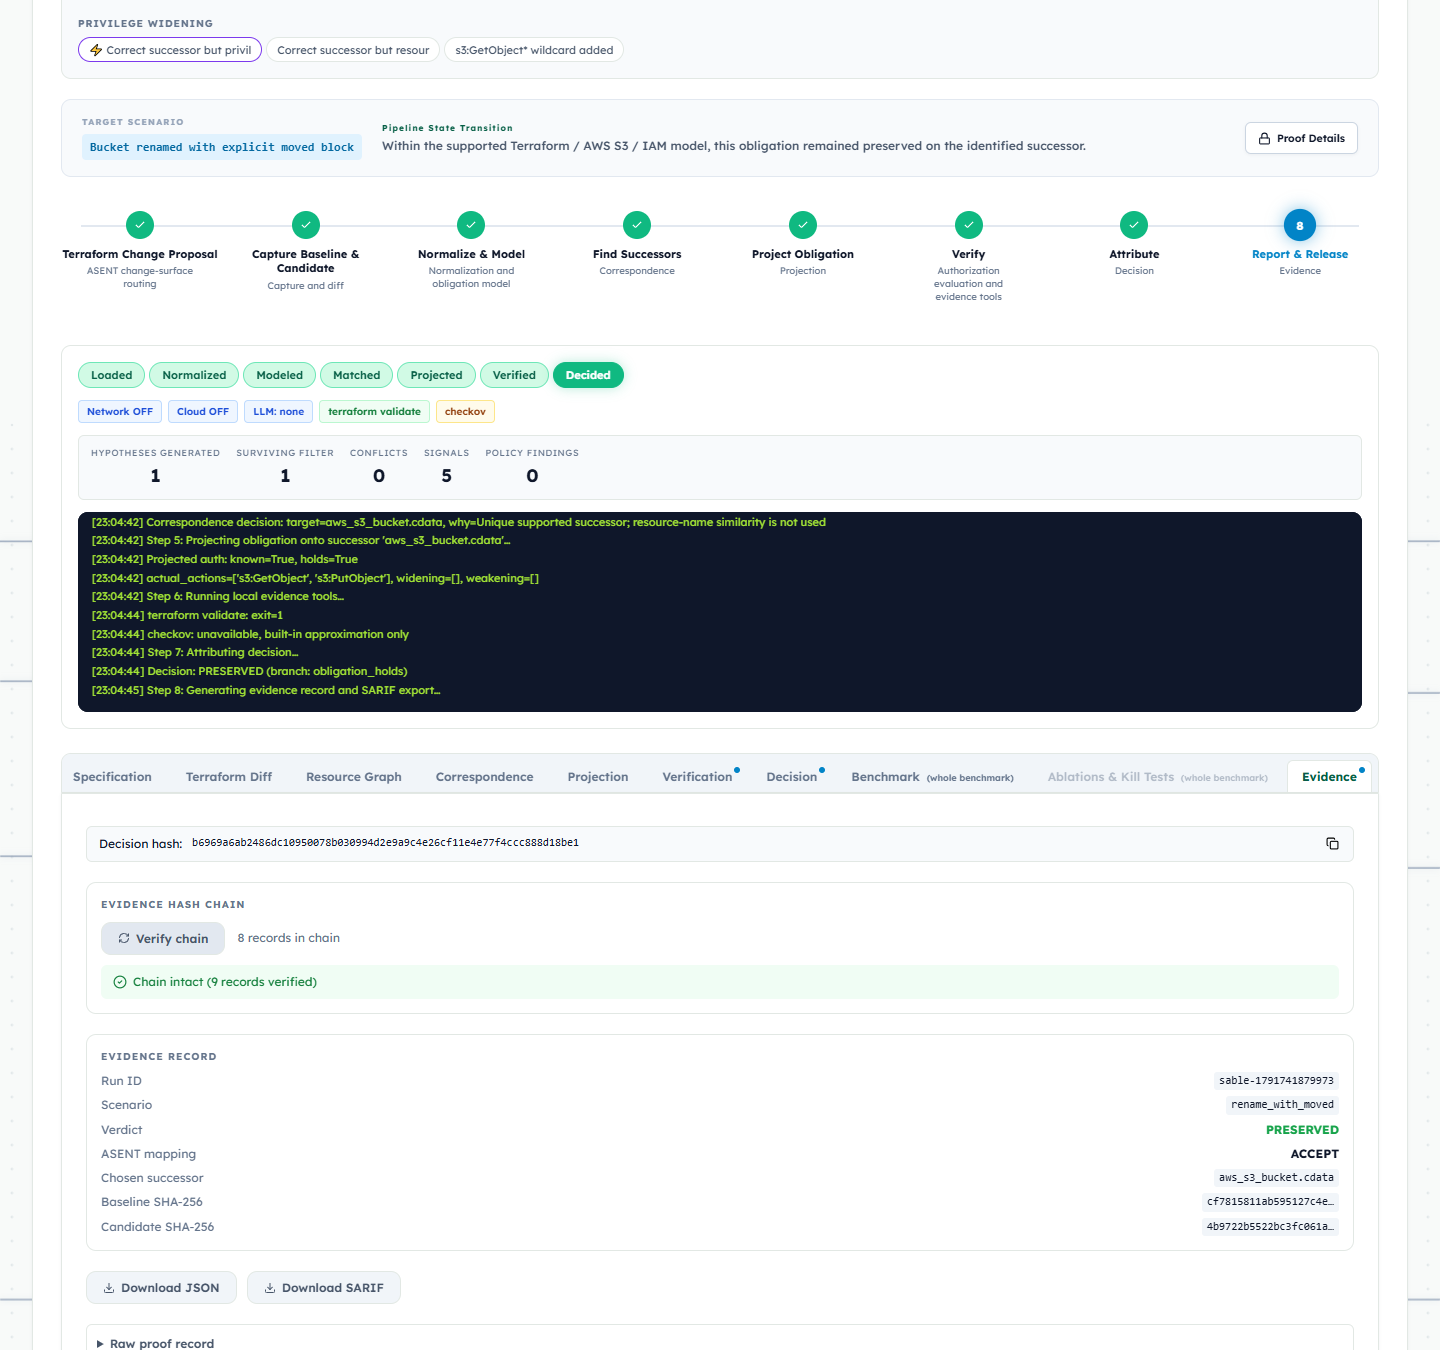
\includegraphics[width=0.98\textwidth,height=0.72\textheight,keepaspectratio]{figures/sable/rename-with-moved-chain-detail.png}
    \caption[SABLE UI: preserved rename with move]{Dedicated SABLE UI evidence for \texttt{rename\_with\_moved}: preserved obligation, SABLE mapping \texttt{ACCEPT}, and an intact chain with nine records verified. Cropped from the original full-page capture for readability.}
    \label{fig:sable-ui-preserved-evidence}
\end{figure}
\clearpage

\begin{figure}[p]
    \centering
    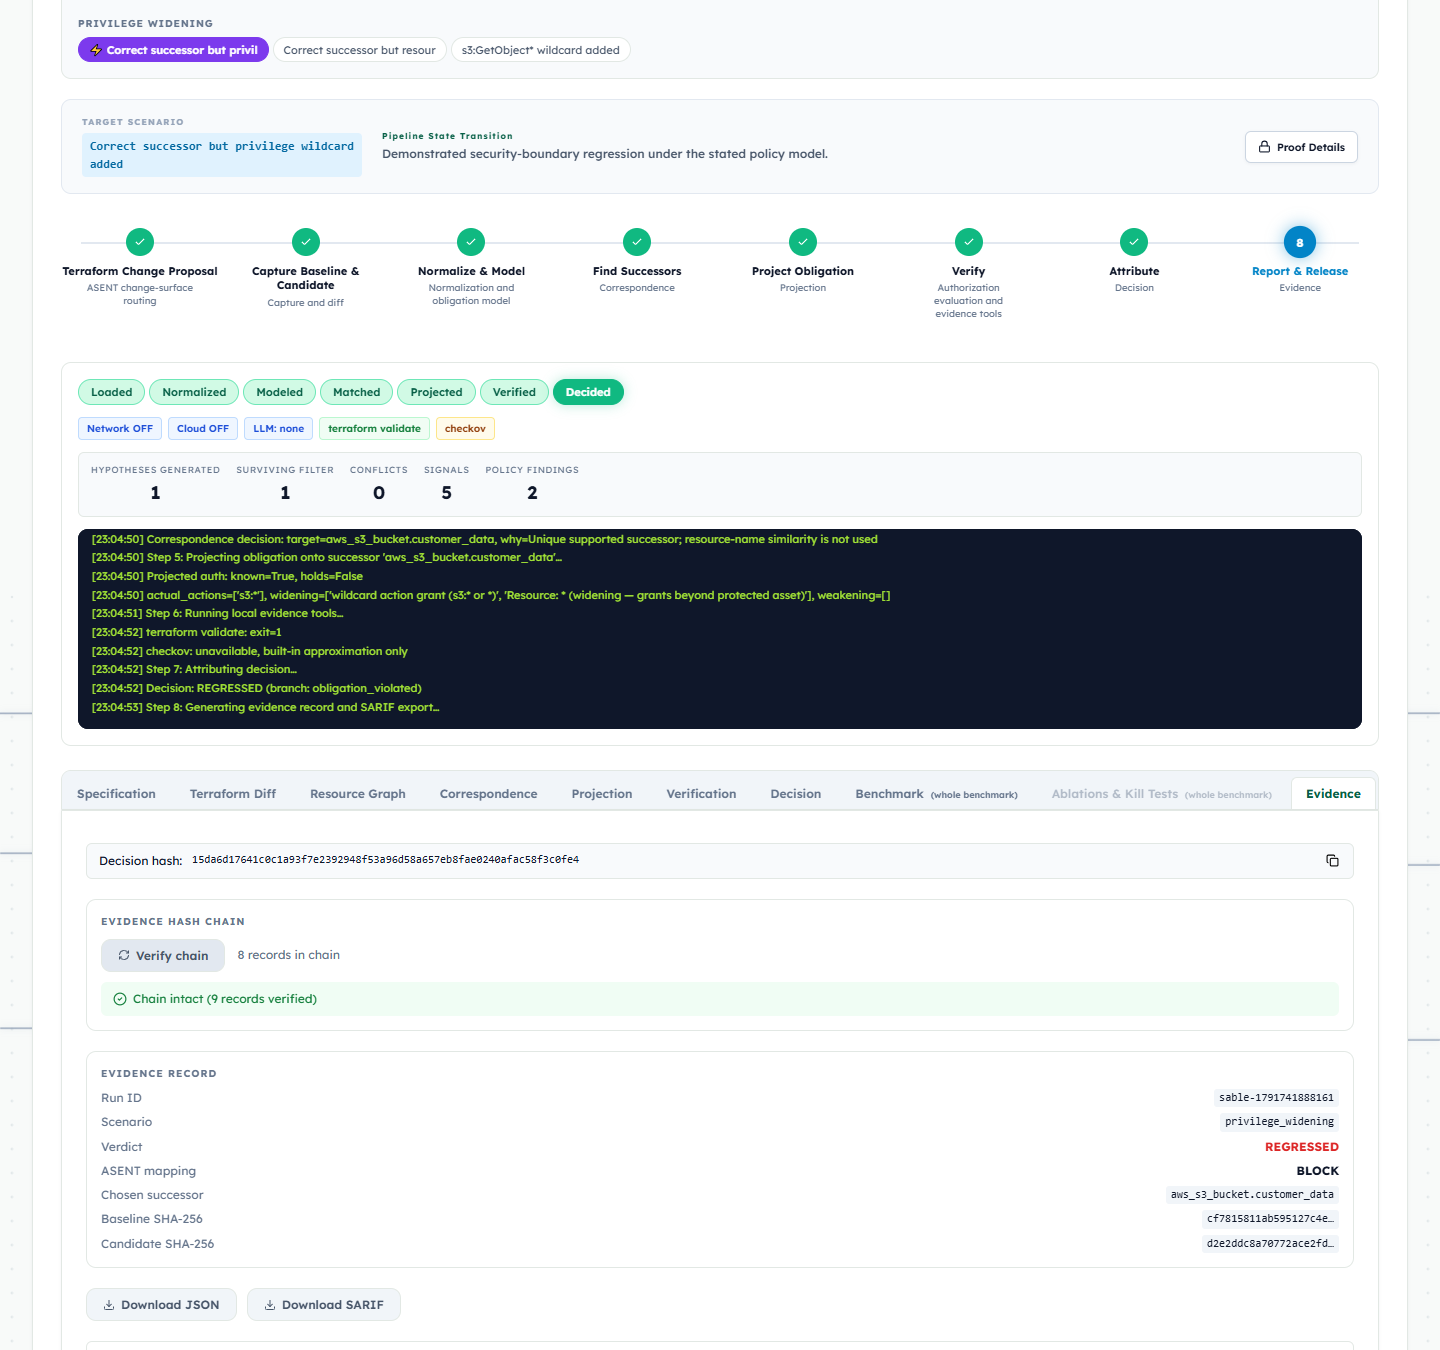
\includegraphics[width=0.98\textwidth,height=0.72\textheight,keepaspectratio]{figures/sable/privilege-widening-chain-detail.png}
    \caption[SABLE UI: privilege widening regression]{Dedicated SABLE UI evidence for \texttt{privilege\_widening}: the widened grant is classified \texttt{REGRESSED}/\texttt{BLOCK}; the evidence chain verifies nine records. Cropped from the original full-page capture for readability.}
    \label{fig:sable-ui-regressed-evidence}
\end{figure}
\clearpage

\begin{figure}[p]
    \centering
    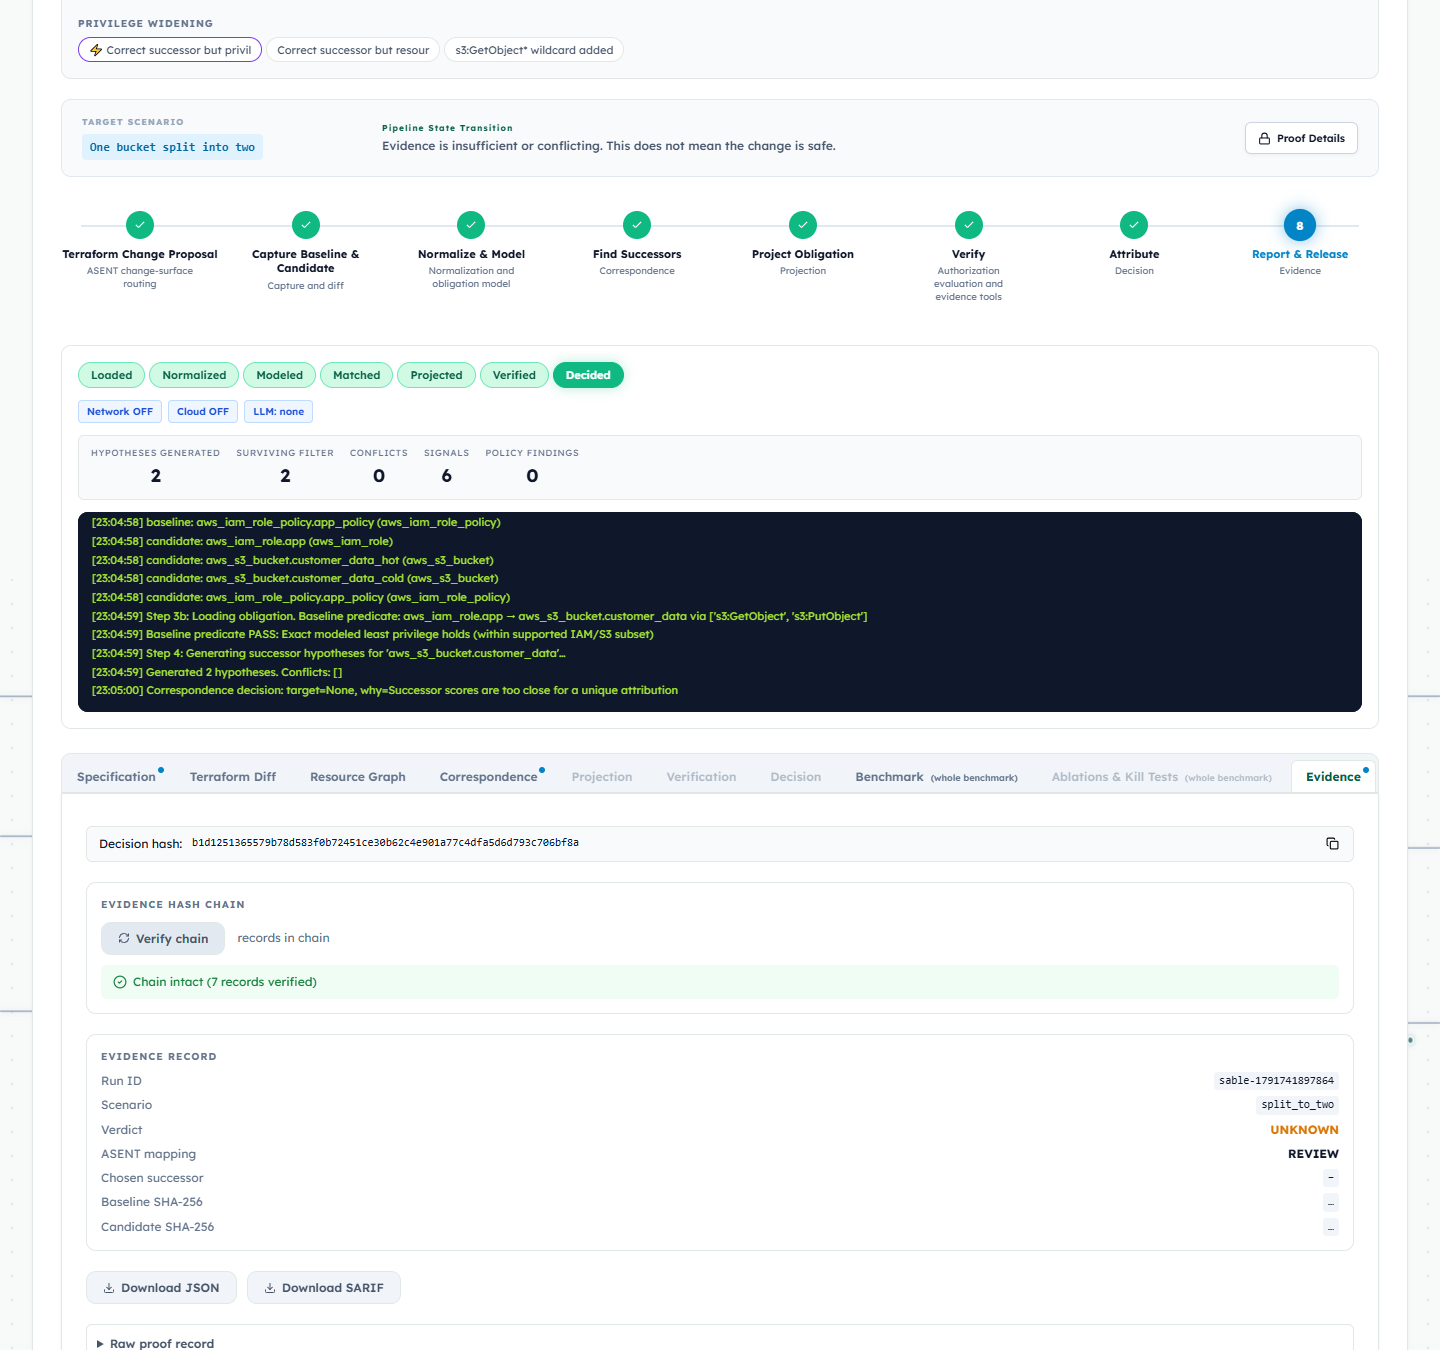
\includegraphics[width=0.98\textwidth,height=0.72\textheight,keepaspectratio]{figures/sable/split-to-two-chain-detail.png}
    \caption[SABLE UI: ambiguous split review]{Dedicated SABLE UI evidence for \texttt{split\_to\_two}: ambiguous correspondence returns \texttt{UNKNOWN}/\texttt{REVIEW}; the evidence chain verifies seven records. Cropped from the original full-page capture for readability.}
    \label{fig:sable-ui-unknown-evidence}
\end{figure}
\clearpage

\begin{figure}[p]
    \centering
    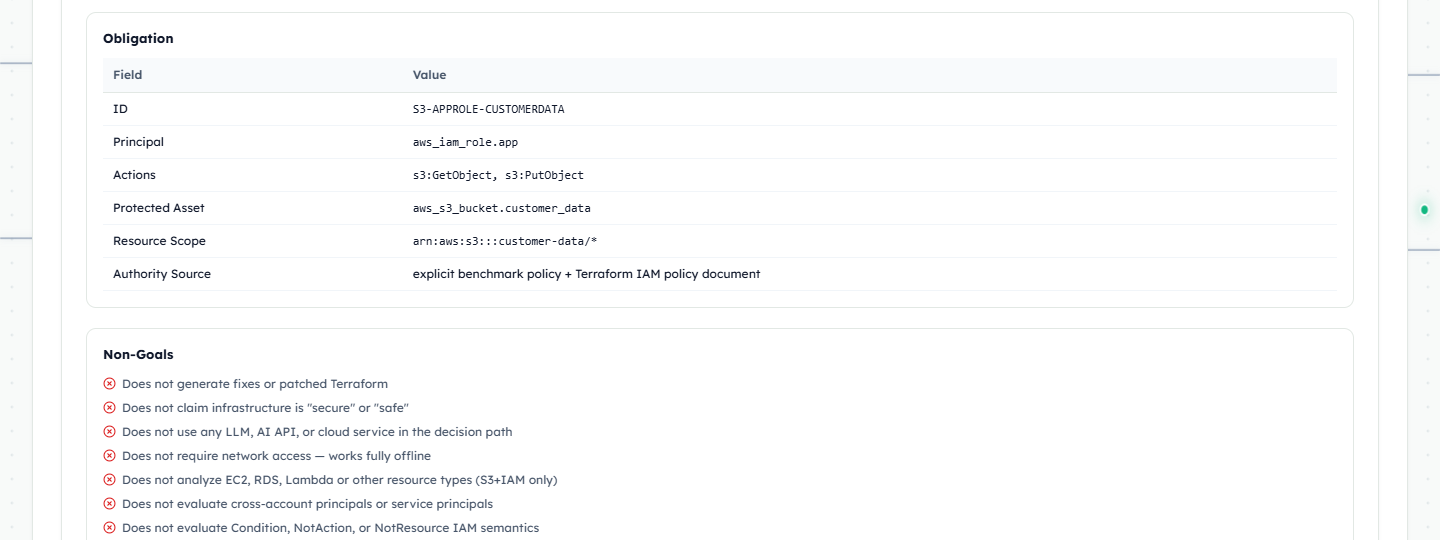
\includegraphics[width=0.96\textwidth,height=0.70\textheight,keepaspectratio]{figures/sable/registered-obligation-detail.png}
    \caption[SABLE UI: registered obligation]{SABLE UI input evidence: the registered \texttt{S3-APPROLE-CUSTOMERDATA} principal, action, and resource scope. This is unaltered UI content cropped to the relevant panel.}
    \label{fig:sable-ui-obligation-and-terraform}
\end{figure}
\clearpage

\begin{figure}[p]
    \centering
    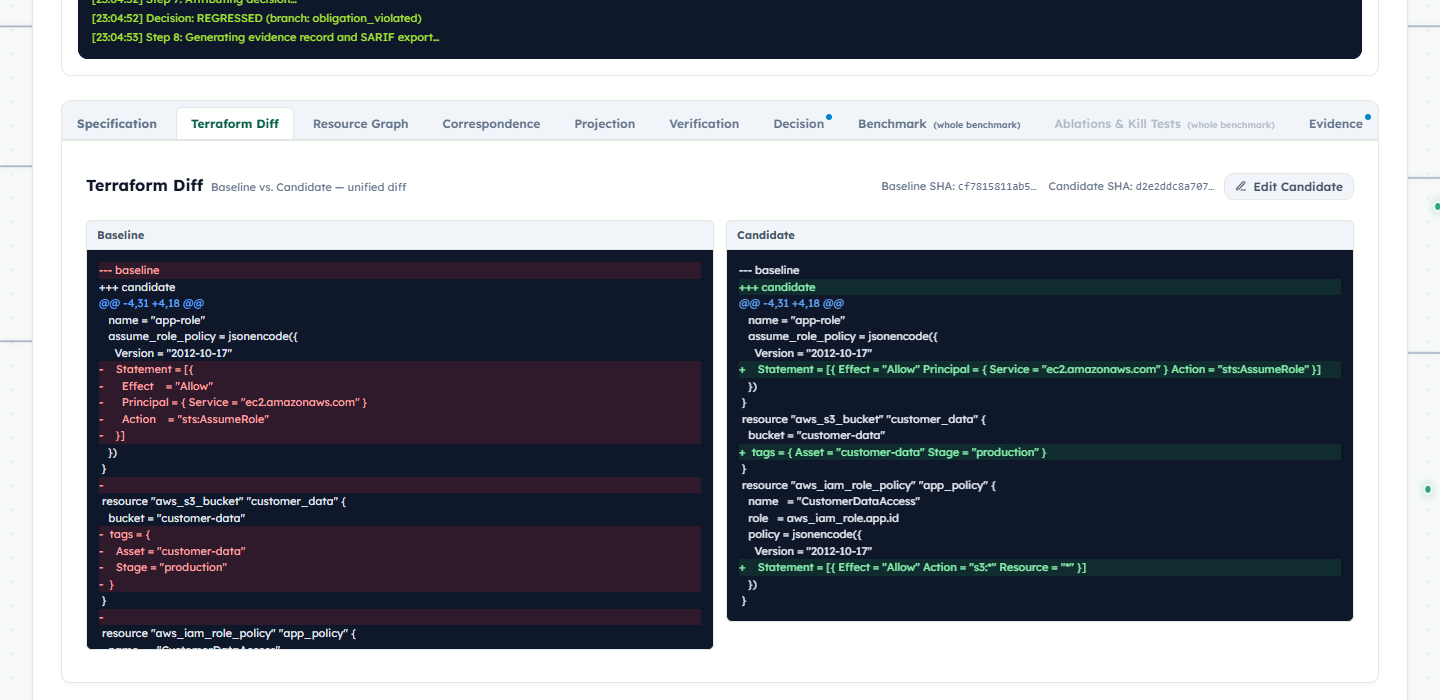
\includegraphics[width=0.96\textwidth,height=0.60\textheight,keepaspectratio]{figures/sable/terraform-diff-detail.png}
    \caption[SABLE UI: Terraform baseline and candidate]{Baseline/candidate Terraform diff shown in the privilege-widening demonstration. The screenshot is cropped to the application panel; the displayed Terraform content is unchanged.}
    \label{fig:sable-ui-terraform-diff}
\end{figure}
\clearpage

\section{Work Remaining}

The following items remain outside the evidence established by the focused SABLE CI run and the three current-checkout rehearsal runs:
\begin{itemize}
    \item broaden and document the supported Terraform and IAM model, including explicit handling for additional resource and policy constructs;
    \item expand independent evaluation beyond the 33 authored synthetic scenarios and investigate false-safe and false-regression cases;
    \item expand integrated Run Workflow validation beyond the three rehearsed scenarios, obtain a refreshed completed-state capture for the unknown run, and investigate the displayed SATRA \texttt{INCONCLUSIVE} result before claiming full-system acceptance;
    \item keep the combined CI workflow green on the integrated branch and verify the report/code branch merge sequence with the team; and
    \item consolidate the team's feedback/action register, design artefacts, and member-by-member contribution evidence in the report appendices.
\end{itemize}

These are remaining or evidence-consolidation tasks, not completed features.

\section{Individual Responsibilities}

The contribution tied to the published SABLE branch is the Terraform infrastructure-security module and the related shared evidence/final-gate integration described in the implementation chapter. Work on the other modules and on shared project artefacts should be attributed using the corresponding module branch, commit, pull request, or review evidence. A module's presence in the inherited repository is not, by itself, proof that a team member authored it during this iteration.

\section{Contribution of Each Team Member}

The checked repository evidence supports the following attribution at this report cut-off:
\begin{longtable}{p{0.29\textwidth}p{0.62\textwidth}}
\toprule
\textbf{Area} & \textbf{Evidence-supported contribution and status}\\
\midrule
SABLE — Muhammad Ali Sajjad (23I-0110) & Terraform/HCL normalization, bounded IAM/S3 authorization, successor matching, scenario tests, and shared-gate evidence integration on the published \texttt{sable} branch. Git history for SABLE files records commits \texttt{adda287}, \texttt{7794336}, and \texttt{7a965b8}; the published milestone is \texttt{9a4dc3d}. Focused CI passed on the published milestone.\\
Shared workflow gate & Evidence freshness/integrity and final-decision behavior are covered by the shared-gate test selection executed with SABLE. Verified by focused tests.\\
CAVR and SATRA-RV ownership & Branch-level ownership has not been verified for this report version; no individual attribution is claimed here.\\
\bottomrule
\end{longtable}

The repository evidence reviewed for this batch supports attribution for SABLE and the shared-gate checks only. Ownership of CAVR and SATRA-RV remains unassigned here until their branch and commit histories have been checked. The integrated screenshot demonstrates their current reported statuses in one run, not ownership or full correctness.

\section{Repository and Version Control Evidence}

\begin{longtable}{p{0.30\textwidth}p{0.61\textwidth}}
\toprule
\textbf{Evidence item} & \textbf{Recorded reference and status}\\
\midrule
Repository branch & \href{https://github.com/SheharyarAli-Dev/Working-POC/tree/sable}{SABLE branch} (available).\\
SABLE commit & \href{https://github.com/SheharyarAli-Dev/Working-POC/commit/9a4dc3d9\allowbreak{}4626ec1f\allowbreak{}14683b74\allowbreak{}20f4640d\allowbreak{}97de20c7}{Commit \texttt{9a4dc3d9}} (pushed).\\
Focused CI run & \href{https://github.com/SheharyarAli-Dev/Working-POC/actions/runs/38058431317}{SABLE shared assurance, run 38058431317} (success).\\
CI/CD pipeline proposal & \href{https://github.com/SheharyarAli-Dev/Working-POC/pull/2}{Pull request 2: Add CI/CD pipeline} (open at check).\\
Verified combined branch & \href{https://github.com/SheharyarAli-Dev/Working-POC/tree/integration/sable-satra-cavr}{integration/sable-satra-cavr} at commit \texttt{665b224}; isolated from \texttt{master}.\\
Combined CI evidence & Core CI 38161406626, SATRA CI 38161406573, and SABLE shared assurance 38161406576 succeeded on the combined commit; see Chapter 8 for run links and test totals.\\
\bottomrule
\end{longtable}

The 44-test run executes the initial focused SABLE/shared-gate selection on commit \texttt{9a4dc3d}; it predates the unresolved-role-binding correction. The CI/CD pull-request status recorded in the earlier SABLE audit is historical and is separate from the successful combined-commit runs listed above.

\section{Milestones and Commit Evidence}

The initial published SABLE milestone was commit \texttt{9a4dc3d}, followed by its focused CI run. The unresolved-role-binding correction was then committed as \texttt{58b0a3d}; it is included in the verified combined commit \texttt{665b224}. The three earlier shared-workflow rehearsal runs at SABLE head \texttt{753a55b} are recorded above. The integration branch establishes which module snapshots were tested together; it does not establish individual ownership for CAVR or SATRA-RV, and it does not supply the official proposal-action records.

\begin{sloppypar}
The narrowly scoped unresolved-role-binding correction in \path{backend/sable/authorization.py} and regression assertions in \path{tests/test_modules.py} were committed as \texttt{58b0a3d} and are included in combined commit \texttt{665b224}. The correction-containing local focused selection passed 27 tests with 10 deselected; see Chapter 8 for its exact command and scope. The initial 44-test CI result is from commit \texttt{9a4dc3d} and does not cover this correction; the combined-snapshot shared-assurance result was 46 passed.
\end{sloppypar}

\section{Tools and Tool-Assisted Development}

The SABLE work and this report update used OpenAI Codex assistance for repository inspection, a narrowly scoped evaluator correction and regression test, and report drafting. AI-assisted output was not treated as proof: the selected tests were executed and their actual result is recorded in Chapter 8. This disclosure covers the SABLE activity known for this contribution; it does not attribute tool use to CAVR, SATRA-RV, or other team members. Each member must confirm their own external/GenAI tools and data handling, and the team must apply the institution's disclosure requirements.

\section{External Components and Dependencies}

The SABLE path uses Python, \texttt{python-hcl2} for parsing Terraform HCL, NetworkX for the resource-reference graph, and the repository's FastAPI/Pydantic API stack. Pytest executes the automated checks, and GitHub Actions provides the recorded CI environment. Terraform CLI, Checkov, Trivy, and Docker/Podman are optional external tools detected by the environment interface; their availability affects the strength or isolation of optional scans. No live AWS API call or infrastructure deployment is used as proof by the SABLE static decision path.

Third-party component versions and notices should be kept aligned with the repository dependency files and \texttt{THIRD\_PARTY\_NOTICES.md}. The report does not claim that an optional scanner ran unless its availability and output are captured in the particular run evidence.

\section{Risks and Mitigation}

\begin{longtable}{p{0.30\textwidth}p{0.61\textwidth}}
\toprule
\textbf{Risk} & \textbf{Mitigation and remaining exposure}\\
\midrule
Wrong logical resource matched after a refactor & Use move, physical-identity, tag, and reference evidence; reject conflicts and close candidate scores. Other Terraform patterns remain uncovered.\\
Policy appears valid but targets the wrong asset & Project the registered obligation onto the chosen successor, not merely the presence of a grant. The IAM/S3 model remains bounded.\\
Unsupported syntax is misclassified as safe & Preserve parse/model limitations and return \texttt{UNKNOWN} when the decision is unsupported. Coverage must expand.\\
Stale or tampered evidence is reused & Check the candidate snapshot, input hash, stale state, and evidence integrity in the shared gate. Broader integration tests remain.\\
Synthetic tests overstate effectiveness & Label the cases as in-house fixtures, not independent or production evaluation. Independent validation remains.\\
Optional scanner is unavailable or weakly isolated & Report tool availability and reduced-strength operation; use container isolation when available. Protection depends on the environment.\\
\bottomrule
\end{longtable}

\section{Security and Privacy Considerations}

The documented SABLE decision path is deterministic, local, and does not put an LLM in the security decision path. The API reports network and cloud access as off for the analysis flow; SABLE compares supplied Terraform snapshots rather than applying them to AWS. The shared orchestrator hashes candidate files and module inputs, and the evidence chain records ordered events with hash links so changes to recorded content can be detected by verification.

Optional scanner isolation is environment-dependent. When container tooling is available, the documented isolation configuration uses no network, a read-only candidate view, a non-root scanner user, and a timeout. If container tooling is unavailable, the environment interface reports native execution rather than implying container isolation. This report does not claim a full sandbox for arbitrary code or a security assessment of deployed cloud resources.

\section{Current Limitations}

The current SABLE model is bounded to the supported Terraform resources and an explicit IAM/S3 policy subset. The parser supports local modules within limits but not all Terraform language features; dynamic module expansion and unsupported expressions are reported as unresolved. It does not establish runtime cloud state, full AWS authorization semantics, or arbitrary semantic equivalence between differently structured Terraform programs. The benchmark scenarios are synthetic and authored in-house. The focused passing CI job establishes the selected SABLE/shared tests only, not full end-to-end product readiness or release-pipeline completion.

\chapter{Remaining FYP Plan}
\section{SABLE Continuation: Proposed Research Work}
The following items describe future SABLE research work, not completed mid-stage features or an approved team schedule. Confirm priorities, owners, dates, and the final evaluation protocol with the supervisor and team.
\begin{enumerate}
    \item Freeze the bounded obligation and scenario labels, then validate the ground truth independently.
    \item Implement and document the strongest agreed comparison baselines; compare B0--B4 and relevant existing tools under a reproducible protocol.
    \item Measure false-safe and false-regression behavior, correspondence outcomes, uncertainty quality, and evidence completeness on a larger controlled corpus.
    \item Extend Terraform/IAM coverage only where justified by the confirmed research question, and preserve explicit unsupported boundaries.
    \item Run broader integrated workflow validation and report any other module's unresolved status separately from SABLE results.
\end{enumerate}
These experiments have not been completed by the focused tests reported in Chapter 8. No performance, novelty, or external-validity conclusion is claimed.

\section{Remaining Scope}
The mid-evaluation implementation is a bounded prototype. SABLE does not cover all Terraform expressions or AWS IAM semantics and does not evaluate deployed cloud state. The team should confirm module-specific remaining scope from each owner's implementation and evidence before setting final-project acceptance criteria.
\section{Remaining Modules and Features}
The verified integration branch combines CAVR, SATRA-RV, SABLE, and the shared workflow. Remaining module work and ownership must be recorded from the team's accepted plans; this report does not infer individual tasks from module presence alone.
\section{Remaining Iterations}
FYP-2 is proposed to focus on the agreed comparative evaluation, stronger independent validation of scenario labels, and additional integration checks. These are future activities, not completed results.
\section{Implementation Plan}
After supervisor and team agreement, record owner-assigned work items for each approved research question, maintain the bounded security models, and review changes against the corresponding requirements and regression tests. No dates or owners are asserted here because an approved schedule was not present in the reviewed records.
\section{Testing and Validation Plan}
\begin{sloppypar}
Retain focused module regressions, Docker-enabled sandbox checks, frontend build/render checks, and the combined suite on the same integration commit. Independently review the benchmark labels and add cases only when their expected result follows from the stated obligation and supported policy model. Report skips and environment limitations alongside every result.
\end{sloppypar}
\section{Deployment Plan}
The current demonstration runs locally with supplied fixtures and does not apply Terraform or contact AWS. Any later deployment or live-cloud evaluation requires a separately approved test environment, credentials policy, and scope; none is claimed for this mid-evaluation report.
\section{Tentative Timeline}
The reviewed repository did not contain an approved FYP-2 calendar or dated owner plan. The team should populate this section from the supervisor-approved schedule rather than infer dates from the current implementation history.
\section{Expected Final Deliverables}
Expected final-project outputs, subject to supervisor approval, are the integrated implementation, traceable requirements/design and test evidence, a reproducible comparative evaluation, and the final report and demonstration. This list is a proposal for planning, not evidence that those deliverables are complete.

\chapter{Conclusion}
For the SABLE mid-stage scope, the implemented prototype addresses refactoring-induced misbinding of a registered S3/IAM security obligation. It checks the trusted baseline, normalizes a bounded Terraform/HCL subset, identifies a supported successor, evaluates the obligation on that successor, and publishes candidate-bound evidence to the shared gate. Controlled tests distinguish \texttt{PRESERVED}, \texttt{REGRESSED}, and \texttt{UNKNOWN}. The correction-containing local selection reported 27 tests passed and 10 deselected; the earlier CI run on commit \texttt{9a4dc3d} reported 44 focused tests passed. Current shared-workflow runs on branch head \texttt{753a55b} recorded \texttt{PRESERVED}/\texttt{REVIEW}, \texttt{REGRESSED}/\texttt{BLOCK}, and \texttt{UNKNOWN}/\texttt{REVIEW}. These are selected correctness checks rather than a full-suite or live-cloud result.

The principal design choice is to keep authorization validity separate from logical-asset correspondence. The focused audit also aligned the standalone evaluator's treatment of unresolved role bindings with the shared evaluator. That correction is commit \texttt{58b0a3d}, included in current branch head \texttt{753a55b}. The current boundaries remain the supported Terraform and IAM/S3 subset, synthetic authored scenarios, and the absence of a completed comparative research evaluation. Future SABLE work is listed in Chapter 10 as proposed research, not completed implementation.

This SABLE conclusion does not supply the missing team-wide research synthesis, confirmed panel action register, contribution records for other modules, administrative confirmations, or complete schedule and meeting evidence. The team must complete those report sections using authoritative records before submission.


\appendix
\chapter{Proposal Action Register}
The team reports that there are no outstanding proposal or panel actions requiring follow-up for this submission. No official Form 10 or signed panel action register was present in the report materials reviewed. This entry records the team's confirmation; it is not an official panel record, and no action items or panel decisions have been inferred.

\chapter{Detailed Requirements}
This appendix preserves the SABLE acceptance trace in a compact form. Requirement identifiers refer to Chapter 4.

\setlength{\tabcolsep}{3pt}
\begin{longtable}{p{0.09\textwidth}p{0.19\textwidth}p{0.32\textwidth}p{0.31\textwidth}}
\toprule
\textbf{ID} & \textbf{\shortstack[l]{Milestone/\\component}} & \textbf{\shortstack[l]{Acceptance\\condition}} & \textbf{\shortstack[l]{Test\\evidence}}\\
\midrule
FR-S1 & I2; HCL parser & Supported resources and local references normalize; unsupported expansion is surfaced. & \path{test_sable_real_hcl}; \path{test_sable_unsupported_terraform_stays_unknown}.\\
FR-S2 & I3; baseline authorization & Registered obligation holds on baseline before continuity can be assessed. & \path{test_sable_real_hcl}; \path{test_sable_unverified_baseline_and_empty_baseline}.\\
FR-S3 & I4; correspondence & Unique supported successor is selected; ambiguous or conflicting candidates abstain. & \path{test_sable_refactor_and_correspondence_cases}.\\
FR-S4 & I4; authorization projection & Correct successor retains required S3 role/action/scope; wrong target and weakened action fail. & \path{test_sable_refactor_and_correspondence_cases}; \path{test_sable_real_hcl}.\\
FR-S5 & I2/I3; bounded semantics & Unsupported semantics and unresolved role attachment remain unknown; known unrelated role binding can be ignored. & \path{test_sable_unsupported_iam_stays_unknown}; \path{test_sable_unresolved_role_binding_with_valid_policy_is_unknown}; evaluator-specific regression tests.\\
FR-S6 & I1; evidence publication & SABLE evidence matches current candidate snapshot and input hash, with valid integrity. & \path{test_shared_sable_evidence_drives_final_gate}.\\
FR-S7 & Shared final gate & Preserved accepts, regression blocks, unknown reviews for the SABLE-only integration cases. & Four parameter cases in \path{test_shared_sable_evidence_drives_final_gate}.\\
FR-S8 & I1; evidence validation & Stale or untrusted evidence cannot establish acceptance. & \path{test_sable_final_gate_rejects_untrusted_evidence}.\\
\bottomrule
\end{longtable}
\setlength{\tabcolsep}{6pt}

The expected labels apply only to the named controlled fixtures and supported policy subset. They do not imply that arbitrary Terraform programs are fully interpreted.

\chapter{Detailed Test Cases}
The local commands and aggregate results are reported in Chapter 7. The cases below identify expected behavior and existing assertion locations; they do not add new test results. The four SABLE shared-gate rows are parameter values of one test function.

\section*{CAVR}
These representative cases trace the implemented fast-gate behavior to existing CAVR tests. They do not claim deep-analysis completion or general malware-detection effectiveness.

\setlength{\tabcolsep}{3pt}
\begin{longtable}{p{0.25\textwidth}p{0.43\textwidth}p{0.22\textwidth}}
\caption{CAVR Detailed Test Cases -- supporting table 1}\\
\toprule
\textbf{Case} & \textbf{Expected observable outcome} & \textbf{Assertion location}\\
\midrule
\endfirsthead
\toprule
\textbf{Case} & \textbf{Expected observable outcome} & \textbf{Assertion location}\\
\midrule
\endhead
Pip request capture & Supported pinned requirements are captured; unsupported forms and malformed requests are reported rather than treated as verified packages. & \path{test_cavr_capture.py}: \path{test_pip_install_with_two_pins}; \path{test_unsupported_forms_are_recorded_not_captured}.\\
Requirement policy gate & A denied, unpinned, unapproved, or lockfile-mismatched package is blocked before download; missing policy remains unresolved. & \path{test_cavr_requirement_gate.py}: \path{test_denylisted_name_is_blocked_even_when_it_is_also_on_the_allowlist}; \path{test_unpinned_requirement_is_blocked}; \path{test_missing_policy_is_unresolved}; \path{test_cavr_pipeline.py}: \path{test_gate_block_makes_zero_downloads}.\\
Artifact integrity & Bytes matching the registry SHA-256 are accepted; altered bytes are rejected and unavailable registry evidence remains unresolved. & \path{test_cavr_pypi_client.py}: \path{test_real_pypdf_wheel_matches_the_recorded_registry_digest}; \path{test_one_flipped_byte_is_rejected}; \path{test_cavr_pipeline.py}: \path{test_registry_unreachable_is_unresolved}.\\
Dependency tree & Pinned compatible dependencies form a tree; missing child pins or a tampered dependency prevent a verified tree. & \path{test_cavr_dep_tree.py}: \path{test_three_level_tree}; \path{test_child_missing_from_the_lockfile_is_unresolved}; \path{test_tampered_leaf_rejects_the_whole_tree}.\\
Advisory check & A recorded affected version is rejected; no advisory data yields an unresolved result. & \path{test_cavr_advisories.py}: \path{test_recorded_pypdf_5_1_0_is_rejected_with_the_advisory_ids}; \path{test_no_data_is_unresolved}; version-range boundaries are checked by \path{test_introduced_fixed_range}.\\
Static wheel scan and capability contract & Aliased sinks are found without importing package code; unsupported scan input and a package without project call-site authority remain unresolved. & \path{test_cavr_ast_scan.py}: \path{test_sink_called_through_an_import_alias_is_still_found}; \path{test_scanning_does_not_execute_the_package}; \path{test_syntax_error_is_an_explicit_finding_and_unresolved}. \path{test_cavr_contract.py}: \path{test_invoicehub_contract_for_pypdf}; \path{test_unused_package_has_no_call_site_authority}.\\
End-to-end gate and wrapper & A verified fixture carries guard evidence; rejected, blocked, and unresolved cases do not invoke pip installation. & \path{test_cavr_pipeline.py}: \path{test_pypdf_6_19_0_is_verified_with_the_guard_evidence}; \path{test_cavr_pip_shim.py}: \path{test_install_on_rejected_never_invokes_pip}; \path{test_install_on_unresolved_never_invokes_pip}.\\
\bottomrule
\end{longtable}
\setlength{\tabcolsep}{6pt}

\section*{SATRA-RV}
These representative cases identify existing SATRA-RV assertions. Their scope is limited to supported Python contracts, fixtures, and the configured execution backend.

\setlength{\tabcolsep}{3pt}
\begin{longtable}{p{0.25\textwidth}p{0.43\textwidth}p{0.22\textwidth}}
\caption{SATRA-RV Detailed Test Cases -- supporting table 2}\\
\toprule
\textbf{Case} & \textbf{Expected observable outcome} & \textbf{Assertion location}\\
\midrule
\endfirsthead
\toprule
\textbf{Case} & \textbf{Expected observable outcome} & \textbf{Assertion location}\\
\midrule
\endhead
Change ingestion & Valid revisions are resolved; hostile references are rejected; added, deleted, and renamed files are represented. & \path{test_satra_ingest.py}: \path{test_added_and_deleted}; \path{test_rename_records_both_paths}; \path{test_hostile_ref_rejected}.\\
Trusted-test integrity & Modified, deleted, planted, or missing trusted test material is detected. & \path{test_satra_trust_and_seed.py}: \path{test_modified_file_is_detected}; \path{test_deleted_file_is_detected}; \path{test_planted_file_is_detected}.\\
Security localization and contract & Supported ownership or SQL changes are localized; missing contract authority yields an inconclusive result. & \path{test_satra_localize.py}: \path{test_astscan_detects_removed_ownership_guard}; \path{test_astscan_detects_string_built_sql}; \path{test_satra_ollama_and_validator.py}: \path{test_missing_contract_produces_inconclusive_never_not_applicable}.\\
Candidate-test validation & Syntax errors, missing or weakened assertions, and contract misalignment are rejected; a valid aligned test is accepted. & \path{test_satra_ollama_and_validator.py}: \path{test_validator_rejects_syntax_error}; \path{test_validator_rejects_weakened_assertion}; \path{test_validator_accepts_valid_test}.\\
Counterfactual oracle check & Supported mutations are generated and evaluated; weakened oracle behavior is distinguished from a genuine assertion failure. & \path{test_satra_counterfactuals.py}: \path{test_mutate_file_ast_ownership}; \path{test_static_integrity_catches_broadened_assertion}; \path{test_satra_ollama_and_validator.py}: \path{test_killed_distinguishes_error_vs_failure}.\\
Decision evidence & Clean evidence can be accepted; weakened-oracle evidence blocks, and the evidence bundle is recorded. & \path{test_satra_decision_and_repair.py}: \path{test_decision_engine_accepts_clean_run}; \path{test_decision_engine_blocks_on_weakened_oracle}; \path{test_decision_engine_evidence_bundle}.\\
Sandbox behavior & The configured container checks enforce network isolation, read-only root, temporary storage, and timeout. & \path{test_satra_sandbox.py}: \path{test_sandbox_network_isolated}; \path{test_sandbox_readonly_root}; \path{test_sandbox_tmpfs_isolated}; \path{test_sandbox_execution_timeout}.\\
Live execution and recommit & Host execution is refused when Docker is unavailable; recommit checks require an approval record and audit checks detect tampering. & \path{test_satra_live_pipeline.py}: \path{test_host_execution_refused_without_docker}; \path{test_satra_recommit.py}: \path{test_recommit_flow_with_local_bare_remote}; \path{test_audit_trail_append_only_and_tamper_detection}.\\
\bottomrule
\end{longtable}
\setlength{\tabcolsep}{6pt}

The appendix identifies existing assertions and expected outcomes, not additional run results. Chapter 7 reports the recorded CI provenance and its limitations.

\clearpage
\section*{SABLE}
\setlength{\tabcolsep}{3pt}
\begin{longtable}{p{0.24\textwidth}p{0.39\textwidth}p{0.26\textwidth}}
\caption{SABLE Detailed Test Cases -- supporting table 3}\\
\toprule
\textbf{Case} & \textbf{Expected observable outcome} & \textbf{Assertion location}\\
\midrule
Supported module refactor, valid obligation & \texttt{PRESERVED}; baseline holds; selected successor and projected authorization hold. & \path{test_sable_real_hcl}; preserved parameters of \path{test_sable_refactor_and_correspondence_cases}.\\
Policy rewritten to wrong bucket & \texttt{REGRESSED}; projected authorization is known and does not hold on successor. & \path{policy_rewrite_wrong_target} parameter of \path{test_sable_refactor_and_correspondence_cases}.\\
Required action weakened & \texttt{REGRESSED}; missing action prevents the obligation from holding. & \path{privilege_weakened_action} parameter of \path{test_sable_refactor_and_correspondence_cases}.\\
Competing successor candidates & \texttt{UNKNOWN}; no unjustified successor attribution. & \path{ambiguous_set_three_candidates} parameter of \path{test_sable_refactor_and_correspondence_cases}.\\
Unsupported IAM Condition & \texttt{UNKNOWN}; projected authorization is not known. & \path{test_sable_unsupported_iam_stays_unknown}.\\
Unresolved dynamic role binding & Standalone and shared evaluators do not claim known safe authorization; SABLE and shared gate yield \texttt{UNKNOWN}/\texttt{REVIEW}. & \path{test_sable_standalone_evaluator_fails_closed_on_unresolved_role_binding}; \path{test_shared_sable_evidence_drives_final_gate}.\\
Known different role binding & Unrelated policy is ignored; intended preserved obligation remains valid. & \path{test_sable_explicitly_unrelated_role_binding_is_ignored}.\\
Unverified baseline & No continuity claim; verdict is \texttt{UNKNOWN}. & \path{test_sable_unverified_baseline_and_empty_baseline}.\\
Shared preserved / regressed / unknown / unresolved-binding cases & Expected pairs: \texttt{PRESERVED}/\texttt{ACCEPT}, \texttt{REGRESSED}/\texttt{BLOCK}, and two \texttt{UNKNOWN}/\texttt{REVIEW}. Evidence is current, input-bound, and integrity-valid. & Four parameter cases in \path{test_shared_sable_evidence_drives_final_gate}.\\
\bottomrule
\end{longtable}
\setlength{\tabcolsep}{6pt}

\chapter{Repository and Contribution Evidence}
\section*{SABLE milestone evidence}
The initial published SABLE implementation milestone is commit \texttt{9a4dc3d}; its focused GitHub Actions run reported 44 passed. The unresolved-role-binding correction and regression tests were committed as \texttt{58b0a3d} and are included in the current \texttt{sable} head, merge commit \texttt{753a55b}. The correction-containing local audit selection reported 27 passed, 10 deselected; it is separate from the earlier CI result.

The shared repository evidence supports the SABLE implementation and shared evidence/final-gate work described in this report. This appendix does not attribute CAVR or SATRA-RV work, infer unrecorded task ownership, or claim the local audit changes were published. Confirm member-by-member contribution records using the team's authoritative task and review history.
A live rehearsal on the current \texttt{sable} checkout at \texttt{753a55b} recorded \texttt{PRESERVED}/\texttt{REVIEW} (run \texttt{b107fd8f0f2f}), \texttt{REGRESSED}/\texttt{BLOCK} (run \texttt{5c6fe1aa3a96}), and \texttt{UNKNOWN}/\texttt{REVIEW} (run \texttt{b6d3588ec006}). All three SABLE evidence records passed integrity and snapshot/input-hash binding checks. The preserved run was reviewed because SATRA returned \texttt{INCONCLUSIVE}; it was not an overall acceptance. The unknown run's stored final gate is complete, while its retained current-checkout UI image is an intermediate display state as described in Chapter 9.

\chapter{Module Evidence Against the Mid-Evaluation Rubric}
\label{app:module-rubric}
The criterion titles below were checked against the official FYP-1 Mid-Evaluation Guidelines and Rubrics (Form~2, pp.~1--2; Form~3, pp.~2--3). This appendix assesses module evidence in the requested order: CAVR, SATRA-RV, then SABLE. It is not a mark prediction or a team-wide compliance statement. \textbf{MET} means repository or CI evidence supports the stated bounded scope; \textbf{PARTIAL} means evidence supports only part of the criterion; \textbf{NOT VERIFIABLE} means repository artifacts cannot establish the requested performance or personal evidence. Contribution attribution follows the report's team-confirmed statements and is not inferred from module presence in Git history.

\setlength{\tabcolsep}{3pt}

\section{CAVR evidence}
\subsection{Form 2: Presentation and Demonstration}
\small
\begin{longtable}{p{0.16\textwidth}p{0.14\textwidth}p{0.62\textwidth}}
\caption{Form 2 rubric evidence -- CAVR}\\
\toprule
\textbf{Criterion} & \textbf{CAVR status} & \textbf{Evidence and limits}\\
\midrule
1. Previous proposal actions addressed (CLO6) & PARTIAL & The report records the team's statement that no actions are outstanding; no signed official action register is included.\\
2. Iteration plan and work breakdown progress (CLO2) & MET for bounded CAVR scope & Chapter~3 milestones map to the implementation described in the CAVR chapters; this does not assert completion of future research evaluation.\\
3. Live prototype with core module demo (CLO4) & MET for recorded scenarios & Chapter~6 records six CAVR API scenarios at commit \texttt{42e2524}, including verified, rejected, blocked, and unresolved outcomes. These are recorded runs, not a new live demonstration.\\
4. Requirements and acceptance criteria (CLO2) & MET for stated requirements & Chapter~4 and Appendices~B--C map FR-C1--FR-C12 to bounded behavior and existing test assertions.\\
5. Design artefacts and evolution (CLO3) & MET for documented design & Chapters~5--6 describe the integrated architecture, CAVR stages, interfaces, and limits; the editable design source is identified in the report.\\
6. Repository, milestones, and member evidence (CLO6) & PARTIAL & Chapter~6 identifies CAVR branch head \texttt{d63183d}; Chapter~7 records run 38137109059. Maryam Fatima's contribution is team-confirmed; Git provenance alone is not used to prove individual ownership.\\
7. Testing and early validation (CLO4) & MET for bounded checks & Chapter~7 records 1,254 passed, zero failed, 26 skipped on the CAVR CI selection and seven separate live tests passed; the skipped live and frontend cases are disclosed.\\
8. Presentation, Q\&A, team participation, and tool ownership (CLO5) & NOT VERIFIABLE & Repository evidence cannot establish oral performance or balanced participation. The report records tool use where established; it does not infer it from commits.\\
\bottomrule
\end{longtable}
\normalsize

\subsection{Form 3: Report Evaluation}
\small
\begin{longtable}{p{0.16\textwidth}p{0.14\textwidth}p{0.62\textwidth}}
\caption{Form 3 rubric evidence -- CAVR}\\
\toprule
\textbf{Criterion} & \textbf{CAVR status} & \textbf{Evidence and limits}\\
\midrule
1. Report format and artefacts (CLO2) & PARTIAL & CAVR requirements, implementation, testing, and evidence are documented; report-wide signatures and official panel records are not supplied by this module evidence.\\
2. Problem formulation, R\&D, and gap analysis (CLO1) & PARTIAL & The CAVR design and literature framing are documented; no completed comparative evaluation or independent effectiveness study is claimed.\\
3. Project vision, scope, and success criteria (CLO2) & MET for bounded scope & Chapter~4 states the package, policy, integrity, and verdict requirements and their unresolved boundaries.\\
4. Requirements and acceptance criteria (CLO2) & MET for mapped requirements & Appendix~B details CAVR FR-C1--FR-C12; Appendix~C identifies representative existing assertions.\\
5. Architecture and component/interface design (CLO3) & MET for documented interfaces & Chapters~5--6 map the module API, dashboard, pipeline, and verification components to the implementation.\\
6. Data, process, and behavior design (CLO3) & MET for bounded behavior & The report documents capture, gate, artifact, dependency, analysis, and verdict stages, including explicit unresolved outcomes.\\
7. Implementation documentation (CLO4) & MET for reported implementation & CAVR Chapters~6--7 and the cited demo material describe source files, interfaces, setup, tests, and limits.\\
8. Testing plan and tool/risk disclosure (CLO5) & PARTIAL & Test scope and external-service, platform, and skip limits are recorded; comparative research and production behavior remain unverified.\\
\bottomrule
\end{longtable}
\normalsize

\section{SATRA-RV evidence}
\subsection{Form 2: Presentation and Demonstration}
\small
\begin{longtable}{p{0.16\textwidth}p{0.14\textwidth}p{0.62\textwidth}}
\caption{Form 2 rubric evidence -- SATRA-RV}\\
\toprule
\textbf{Criterion} & \textbf{SATRA-RV status} & \textbf{Evidence and limits}\\
\midrule
1. Previous proposal actions addressed (CLO6) & PARTIAL & The report records the team's statement that no actions are outstanding; no signed official action register is included.\\
2. Iteration plan and work breakdown progress (CLO2) & MET for bounded SATRA scope & Chapters~3 and 6 document the implementation milestones and the distinct shared-analyzer and dedicated-pipeline paths.\\
3. Live prototype with core module demo (CLO4) & PARTIAL & The dedicated UI and recorded replay are described, but the report explicitly records no fresh SATRA-specific browser capture. Shared workflow rehearsals returned SATRA INCONCLUSIVE.\\
4. Requirements and acceptance criteria (CLO2) & MET for stated requirements & Chapter~4 and Appendices~B--C map FR-SATRA-01--FR-SATRA-11 to implementation paths and existing assertions.\\
5. Design artefacts and evolution (CLO3) & MET for documented design & Chapter~5 and the editable diagram source document the shared architecture and SATRA analysis flow.\\
6. Repository, milestones, and member evidence (CLO6) & PARTIAL & Chapter~7 identifies exact tested PR~\#5 head \texttt{554b6d5} and CI run 38260995764. Syed Sheharyar Ali's contribution is team-confirmed; individual ownership is not inferred from Git history.\\
7. Testing and early validation (CLO4) & MET for bounded checks & Exact-head CI recorded 84 focused tests passed and four required Docker checks without skips. Later selector mapping has no dedicated unit test identified in the report.\\
8. Presentation, Q\&A, team participation, and tool ownership (CLO5) & NOT VERIFIABLE & Repository evidence cannot establish oral performance, balanced participation, or individual understanding.\\
\bottomrule
\end{longtable}
\normalsize

\subsection{Form 3: Report Evaluation}
\small
\begin{longtable}{p{0.16\textwidth}p{0.14\textwidth}p{0.62\textwidth}}
\caption{Form 3 rubric evidence -- SATRA-RV}\\
\toprule
\textbf{Criterion} & \textbf{SATRA-RV status} & \textbf{Evidence and limits}\\
\midrule
1. Report format and artefacts (CLO2) & PARTIAL & SATRA requirements, implementation, tests, and evidence are documented; report-wide signatures and official panel records are not established by module evidence.\\
2. Problem formulation, R\&D, and gap analysis (CLO1) & PARTIAL & The bounded Python security-contract problem and research framing are documented; completed comparative evaluation and broad framework coverage are not claimed.\\
3. Project vision, scope, and success criteria (CLO2) & MET for bounded scope & Chapters~1, 3, and 4 state supported contract, test, counterfactual, execution, and decision boundaries.\\
4. Requirements and acceptance criteria (CLO2) & MET for mapped requirements & Appendix~B traces SATRA functional requirements; Appendix~C identifies representative existing test assertions.\\
5. Architecture and component/interface design (CLO3) & MET for documented interfaces & Chapters~5--6 describe module API, UI, shared analyzer, dedicated pipeline, and their different evidence paths.\\
6. Data, process, and behavior design (CLO3) & MET for bounded behavior & The SATRA flow, trust checks, localization, contract, sandboxed execution, validation, and decision stages are documented with uncertainty limits.\\
7. Implementation documentation (CLO4) & MET for reported implementation & SATRA Chapters~6--7 document source components, setup, interface, test scope, and current limitations.\\
8. Testing plan and tool/risk disclosure (CLO5) & PARTIAL & CI provenance, sandbox checks, skips, local setup errors, and missing fresh browser capture are disclosed; untested selector mapping and broad coverage remain limitations.\\
\bottomrule
\end{longtable}
\normalsize

\section{SABLE evidence}
SABLE evidence retains its exact commit and run provenance. Its 2026-10-14 shared-workflow rehearsals recorded preserved, regressed, and unknown module outcomes, with aggregate REVIEW, BLOCK, and REVIEW because SATRA was INCONCLUSIVE; no overall ACCEPT is claimed. The machine-readable evidence is \path{report/evidence/run-workflow-current-master-2026-10-14.json}. No fresh SABLE screenshot was produced for that later report pass. Focused and integration totals retain their original source commits and are not described as tests of this report revision.

\subsection{Form 2: Presentation and Demonstration}
\small
\begin{longtable}{p{0.17\textwidth}p{0.13\textwidth}p{0.64\textwidth}}
\caption{Form 2: Presentation and Demonstration -- supporting table 1}\\
\toprule
\textbf{Criterion} & \textbf{SABLE status} & \textbf{Files, commits, tests, CI, and demonstration evidence}\\
\midrule
\endfirsthead
\toprule
\textbf{Criterion} & \textbf{SABLE status} & \textbf{Files, commits, tests, CI, and demonstration evidence}\\
\midrule
\endhead
1. Previous proposal actions addressed (CLO6) & PARTIAL & The team reports no outstanding proposal or panel actions, and the SABLE contributor reports that no SABLE-specific action was communicated after proposal re-defense. No official signed action register was found. This team-reported status is not represented as an official panel record.\\
2. Iteration plan and work breakdown progress (CLO2) & MET for SABLE I1--I4 & \path{chapter3_iteration_plan.tex} maps SABLE milestones to the implementation. Relevant source includes \path{backend/sable/analyzer.py}, \path{hcl_parser.py}, \path{correspondence.py}, and \path{authorization.py}. The milestone changes are present in \texttt{84f91a9} and exact tested PR head \texttt{554b6d5}. The bounded selection on the correction-containing local tree recorded 27 passed and 10 deselected; focused shared-assurance CI on \texttt{84f91a9} passed 48 tests (run \href{https://github.com/SheharyarAli-Dev/Working-POC/actions/runs/38220597576}{38220597576}). Shared dashboard runs \texttt{21adc601d6b7} and \texttt{0849603bfc16} demonstrate preserved and wrong-target outcomes (Chapter~9/runbook).\\
3. Live prototype with core module demo (CLO4) & MET for bounded SABLE demo & The integrated UI is \path{frontend/src/components/SableModule.tsx} and shared workflow page is \path{frontend/src/components/RunWorkflowModule.tsx}. Persisted runs \texttt{21adc601d6b7} and \texttt{0849603bfc16} show SABLE \texttt{PRESERVED}/overall \texttt{REVIEW} and SABLE \texttt{REGRESSED}/overall \texttt{BLOCK}; retained images are \path{report/evidence/asent-sable-preserved-live.png} and \path{report/evidence/asent-sable-regressed-live.png}. Evidence binding is documented for both. The preserved overall \texttt{REVIEW} is due to SATRA \texttt{INCONCLUSIVE}; no AWS apply or live authorization call was made.\\
4. Requirements and acceptance criteria (CLO2) & MET for bounded SABLE requirements & \path{chapter4_requirements.tex} and Appendix~B define FR-S1--FR-S8 with named tests and expected \texttt{PRESERVED}, \texttt{REGRESSED}, and \texttt{UNKNOWN} outcomes. Implementation is in \path{backend/sable/}; tests are in \path{tests/test_modules.py} and \path{tests/test_integration.py}. The 27-pass local selection and 48-pass focused CI on \texttt{84f91a9} are distinct records; four shared-gate cases assert final outcomes and input/snapshot bindings. The runbook records live preserved/regressed demonstrations.\\
5. Design artefacts and evolution (CLO3) & MET for SABLE artefacts & The editable external source \texttt{ASENT\_All\_Diagrams.drawio} pages 02, 07, and 08 supplies the architecture, SABLE process, and domain figures in Chapter~5. Source-grounded interfaces are in \path{backend/sable/analyzer.py}, \path{correspondence.py}, and \path{policy_semantics.py}; the unresolved-binding change is \texttt{58b0a3d} and the later gate corrections are in \texttt{84f91a9}. Regression tests cover unresolved versus statically unrelated role bindings. Exact-head CI passed all 18 PR checks.\\
6. Repository, milestones, and member evidence (CLO6) & MET for SABLE contribution & Chapter~9 records SABLE milestone commits and exact merge provenance; \path{backend/sable/}, \path{tests/}, and PR~\#5 head \texttt{554b6d5} are the implementation record. CI runs \href{https://github.com/SheharyarAli-Dev/Working-POC/actions/runs/38260995657}{38260995657} (SABLE shared assurance) and the linked Core/SATRA checks passed on the exact PR head. The SABLE status makes no attribution claim for CAVR/SATRA or other team members.\\
7. Testing and early validation (CLO4) & MET for bounded validation & Focused tests cover real HCL, refactor/correspondence, wrong target, weakened action, unresolved policy, invalid baseline, and shared gate. On source commit \texttt{84f91a9}, shared-assurance CI recorded 48 passing tests (run \href{https://github.com/SheharyarAli-Dev/Working-POC/actions/runs/38220597576}{38220597576}); all 18 PR checks passed on exact head \texttt{554b6d5}. The local Windows full suite had 36 failures and 12 setup errors and is reported as such. Live demo runs are linked in Criterion~3. This is early controlled validation, not full AWS/Terraform semantics or an independent accuracy study.\\
8. Presentation, Q\&A, team participation, and tool ownership (CLO5) & NOT VERIFIABLE & Chapter~9 and \path{docs/sable/tool-disclosure.md} record the established SABLE tool use. A repository cannot verify oral Q\&A, balanced participation, or an individual's understanding. These personal performance criteria are not inferred from commits, tests, CI runs, or screenshots.\\
\bottomrule
\end{longtable}
\normalsize

\subsection{Form 3: Report Evaluation}
\small
\begin{longtable}{p{0.17\textwidth}p{0.13\textwidth}p{0.64\textwidth}}
\caption{Form 3: Report Evaluation -- supporting table 2}\\
\toprule
\textbf{Criterion} & \textbf{SABLE status} & \textbf{Files, commits, tests, CI, and demonstration evidence}\\
\midrule
\endfirsthead
\toprule
\textbf{Criterion} & \textbf{SABLE status} & \textbf{Files, commits, tests, CI, and demonstration evidence}\\
\midrule
\endhead
1. Report format and artefacts (CLO2) & PARTIAL & The editable source includes the report chapters, requirements, tests, implementation evidence, figures, sources, and rubric appendix. The report workflow and final artifact are checked for this revision. The individual signature lines are unsigned, and no signed panel or meeting record is included. These administrative items are outside repository implementation evidence.\\
2. Problem formulation, R\&D, and gap analysis (CLO1) & PARTIAL for SABLE & Chapters~1--2 and \path{report/sources/SABLE_design.txt} state the bounded continuity problem, literature context, and proposed comparisons. Commits \texttt{84f91a9}/\texttt{554b6d5}, test evidence, and the preserved/regressed demos verify implementation behavior only. No completed comparative B0--B4 study or independent research advantage is claimed.\\
3. Project vision, scope, and success criteria (CLO2) & MET for SABLE scope & Chapters~1, 3, and 4 define the S3/IAM obligation, supported Terraform subset, I1--I4 milestones, and observable three-way outcomes. \path{backend/sable/} and the named tests implement these checks; focused CI on \texttt{84f91a9}, exact-head CI on \texttt{554b6d5}, and the preserved/regressed shared runs provide implementation evidence. The demo is bounded and uses no live AWS.\\
4. Requirements and acceptance criteria (CLO2) & MET for SABLE requirements & \path{chapter4_requirements.tex} and Appendix~B map FR-S1--FR-S8 to source and tests. \path{tests/test_modules.py} and \path{tests/test_integration.py::test_shared_sable_evidence_drives_final_gate} cover expected decisions and evidence binding. Focused CI run \href{https://github.com/SheharyarAli-Dev/Working-POC/actions/runs/38220597576}{38220597576} passed 48 tests on \texttt{84f91a9}; all 18 checks passed on exact PR head \texttt{554b6d5}.\\
5. Architecture and component/interface design (CLO3) & PARTIAL for team report; SABLE evidence present & Chapter~5 Figure~\ref{fig:asent-overall-architecture} uses editable-source page 02 and maps React, FastAPI, orchestration, CAVR/SATRA/SABLE, evidence storage, and the shared gate to the local source tree. \path{backend/orchestrator/service.py}, \path{backend/orchestrator/final_gate.py}, and module API/analyzer files ground the interfaces. Exact-head CI and shared workflow runs exercise the integrated route; reconciliation of team-wide ownership/interfaces remains outside the SABLE-only evidence.\\
6. Data, process, and behavior design (CLO3) & MET for SABLE artefacts & Chapter~5 Figures~\ref{fig:sable-current-process} and \ref{fig:sable-domain-model} use editable-source pages 07 and 08. \path{hcl_parser.py}, \path{correspondence.py}, \path{authorization.py}, and \path{policy_semantics.py} implement the bounded flow; tests cover baseline, successors, projection, uncertainty, and gate binding. Source commit \texttt{84f91a9}, focused CI run \texttt{38220597576}, exact PR head \texttt{554b6d5}, and live preserved/regressed runs support the stated SABLE behavior.\\
7. Implementation documentation (CLO4) & MET for SABLE content & Chapter~6 describes SABLE files, algorithms, Windows setup, interfaces, and semantic limits; \path{docs/sable/} provides implementation and demo notes. The source is at \texttt{554b6d5}/merge \texttt{ffe8aa91}; focused SABLE tests, 48-test CI, 18 exact-head checks, and the two retained shared-workflow captures provide reproducible evidence.\\
8. Testing plan and tool/risk disclosure (CLO5) & PARTIAL & Chapter~8 gives exact test and CI provenance, including Windows failures/errors and Linux Docker checks; Chapter~9 and \path{docs/sable/tool-disclosure.md} record established tools and limits. The CI run \texttt{38220597576} belongs to \texttt{84f91a9}; exact merged-head checks are \texttt{554b6d5}. Runs \texttt{21adc601d6b7}/\texttt{0849603bfc16} show module and aggregate statuses separately. No comparison experiment, live cloud deployment, or production behavior is asserted.\\
\bottomrule
\end{longtable}
\normalsize

\setlength{\tabcolsep}{6pt}
The full scenario identifiers, images, exact test command, and run links are recorded in \path{report/evidence/SABLE_MID_DEMO_RUNBOOK.md}. The statuses here are module-scope evidence only; team-wide marks, signatures, and oral presentation are not inferred from repository records.

\chapter{Additional Design Diagrams}
The report presents a shared ASENT architecture and gate, a cross-module use-case view, CAVR and SABLE process diagrams, the integrated assurance sequence, and a shared data model in Chapters~4 and~5. Chapter~6 includes the SATRA-RV live-pipeline sequence and state diagrams; Chapter~9 includes the repository CI/CD view. The twelve added diagrams are PNG renderings supplied in \path{diagram\_replacements\_2026-10-21/preview\_v2/report-diagrams-branch}; they are trimmed only to remove surrounding whitespace. Editable DOT and Mermaid source files are retained in \path{report/diagrams/src/}.

\chapter{Meeting and Progress Evidence}
No supervisory meeting minutes or signed progress records were included in the report-source archive or the SABLE repository evidence reviewed for this update. Do not infer meeting dates, decisions, or feedback from implementation history. The team should add authoritative meeting/progress records here if required by the rubric and confirm which project decisions were approved.


\bibliographystyle{IEEEtran}
\bibliography{references/references}
\end{document}

